\documentclass{article}
\usepackage{iclr2026_conference,times}
\input{math_commands.tex}
\iclrfinalcopy

\usepackage{graphicx}
\definecolor{mylinkcolor}{RGB}{11, 20, 110}
\usepackage[
    pagebackref,
    breaklinks,
    citecolor=mylinkcolor,
    colorlinks=true,
    linkcolor=mylinkcolor,
    urlcolor=mylinkcolor
]{hyperref}

\usepackage{amsthm}
\usepackage{booktabs}
\usepackage{algorithm}
\usepackage{algorithmic}
\usepackage{wrapfig}
\usepackage[table,dvipsnames]{xcolor}
\usepackage{multirow} 
\usepackage{xspace}
\usepackage[breakable]{tcolorbox}
\usepackage{titletoc}
\usepackage{tabularx}
\usepackage{subcaption}
\usepackage{enumitem}

\newcommand{\model}{\textsc{AgentFlow}\xspace}

\makeatletter
\renewcommand{\paragraph}{\@startsection{paragraph}{4}{\z@}{0.0ex plus
0.3ex minus .2ex}{-1em}{\normalsize\textbf}}
\makeatother

\definecolor{darkgreen}{RGB}{0, 181, 18}
\definecolor{darkred}{RGB}{252, 90, 90}

\definecolor{DeltaBg}{HTML}{D4F2D7}
\definecolor{SearchBg}{HTML}{C2E6F5}
\definecolor{AgenticBg}{HTML}{F5C2CC}
\definecolor{MathBg}{HTML}{E6D4F2}
\definecolor{ScienceBg}{HTML}{FBE0BC}

\newcommand{\gain}[1]{$\uparrow$ #1}
\newcommand{\mygreen}[1]{\cellcolor{darkgreen!#1}}

\definecolor{toolcardbox}{RGB}{240, 248, 255}
\definecolor{toolcardborder}{RGB}{52, 52, 173}

\newtcolorbox{custombox}[2][]{
    colback=toolcardbox,
    colframe=toolcardborder,          
    coltitle=white,                
    arc=1pt,                       
    boxrule=1pt,
    fonttitle=\bfseries,
    title=#1,                      
    left=5pt,
    right=5pt,
    top=5pt,
    bottom=5pt,
    before skip=1em,
    after skip=1em,
    fontupper=\small,               
    breakable,     
    width=1.\linewidth, 
    #1                        
}

\newtcolorbox{tooldescbox}[1]{%
    colback=toolcardbox,
    colframe=toolcardborder,
    arc=1pt,                       
    boxrule=1pt,
    left=5pt,
    right=5pt,
    top=5pt,
    bottom=5pt,
    fonttitle=\bfseries,
    title={Tool Metadata of #1},
    fontupper=\small,             
    breakable,
}

\newtcolorbox{limitationbox}{%
    colback=failbg,
    colframe=failframe,
    arc=1pt,                      
    boxrule=0.8pt,
    left=4pt,
    right=4pt,
    top=4pt,
    bottom=4pt,
    fonttitle=\bfseries\small,
    title={Limitation},
    coltitle=white,
    fontupper=\small,               
    breakable,
    before skip=6pt,
    after skip=6pt
}

\newtcolorbox{bestpracticebox}{%
    colback=successbg,
    colframe=successframe,
    arc=1pt,                        
    boxrule=0.8pt,
    left=4pt,
    right=4pt,
    top=4pt,
    bottom=4pt,
    fonttitle=\bfseries\small,
    title={Best Practice},
    coltitle=white,
    fontupper=\small,              
    breakable,
    before skip=6pt,
    after skip=6pt
}

\newcommand{\inputtype}[1]{\textbf{Input:} #1}
\newcommand{\outputtype}[1]{\textbf{Output:} #1}
\newcommand{\smalltt}[1]{{\ttfamily\fontsize{8}{10}\selectfont #1}}

\definecolor{failbg}{RGB}{248, 230, 234}
\definecolor{failframe}{RGB}{176, 36, 24}

\definecolor{successbg}{RGB}{239, 255, 229}
\definecolor{successframe}{RGB}{34, 139, 34}

\newlist{toolenum}{enumerate}{2}
\setlist[toolenum]{label=\arabic*., leftmargin=1.8em, itemsep=2pt, topsep=4pt}

\newtcolorbox{simplecode}[1][]{%
    colback=toolcardbox,
    colframe=toolcardbox,
    arc=1pt,
    boxrule=0pt,
    top=-3pt, bottom=0pt,
    left=3pt, right=3pt,
    boxsep=0pt,
    left skip=0pt,
    right skip=0pt,
    fontupper=\ttfamily\fontsize{8.0}{10}\selectfont,
    breakable,
    #1
}

\newtcolorbox{casebox}[3]{
    colback=#1,             
    colframe=#2,    
    arc=1pt,
    coltitle=white,                  
    fonttitle=\bfseries,         
    title=#3,                    
    boxrule=1pt,                   
    rounded corners,   
    breakable
}

\newtcolorbox{casecode}[1]{%
    colback=#1,
    colframe=toolcardbox,
    arc=1pt,
    boxrule=0pt,
    top=-3pt, bottom=0pt,
    left=3pt, right=3pt,
    boxsep=0pt,
    left skip=0pt,
    right skip=0pt,
    fontupper=\ttfamily\fontsize{8.0}{10}\selectfont,
    breakable,
}

\newtheoremstyle{mythm}%
  {3pt}{3pt}{\itshape}{}{\bfseries}{.}{ }{}
\newtheoremstyle{mydef}%
  {3pt}{3pt}{}{}{\bfseries}{.}{ }{}

\theoremstyle{mydef}
\newtheorem{definition}{Definition}[section]

\theoremstyle{mythm}
\newtheorem{theorem}{Theorem}[section]
\newtheorem{lemma}[theorem]{Lemma}

\title{In-the-Flow Agentic System Optimization for Effective Planning and Tool Use}

\author{
  \hspace{-1mm}\textbf{Zhuofeng Li}$^{*1,2}$\textnormal{,} 
  \textbf{Haoxiang Zhang}$^{*1,3}$\textnormal{,}  
  \textbf{Seungju Han}$^{1}$\textnormal{,}  
  \textbf{Sheng Liu}$^{1}$\textnormal{,}  
  \textbf{Jianwen Xie}$^{4}$\textnormal{,}  \\
  \textbf{Yu Zhang}$^{2}$, 
  \textbf{Yejin Choi}$^{1}$, 
  \textbf{James Zou}$^{\dagger1}$, 
  \textbf{Pan Lu}$^{*\dagger1}$ \\
  $^1$Stanford University, 
  $^2$Texas A\&M University, 
  $^3$UC San Diego,
  $^4$Lambda \vspace{-1mm}
  \\\\
  \begin{minipage}[t]{0.1\textwidth}
      \centering
      \href{https://agentflow.stanford.edu}{
\includegraphics[height=2.5em]{logos/agentflow.pdf}}
  \end{minipage}%
  \hfill
  \hspace{-5mm}
  \begin{minipage}[t]{0.7\textwidth}
      \vspace{-8.5mm} 
      \textbf{\texttt{Website:}}
      \textbf{\url{https://agentflow.stanford.edu}\vspace{1mm}}
      \\
      \raisebox{-0.4ex}{
\includegraphics[height=1em]{logos/github.png}}\hspace{0.3em}\href{https://github.com/lupantech/AgentFlow}{\texttt{Code}} 
      \hspace{0.2cm}
      \raisebox{-0.4ex}{
\includegraphics[height=1em]{logos/huggingface.png}}\hspace{0.3em}\href{https://huggingface.co/AgentFlow/models}{\texttt{Model}}
      \hspace{0.2cm}
      \raisebox{-0.4ex}{
\includegraphics[height=1em]{logos/gradio.png}}\hspace{0.3em}\href{https://huggingface.co/spaces/AgentFlow/agentflow}{\texttt{Demo}}
      \hspace{0.2cm}
      \raisebox{-0.4ex}{
\includegraphics[height=1em]{logos/agentflow.pdf}}\hspace{0.4em}\href{https://agentflow.stanford.edu/\#visualization}{\texttt{Visualize}}
  \end{minipage}
    \vspace{-7mm}
}

\begin{document}
\maketitle
\renewcommand*\thefootnote{}
\footnotetext[0]{
    *Equal contribution.
    $^{\dagger}$Co-senior authors. 
    Work was partially done while ZL and HZ were visiting Stanford.
}

\begin{abstract}
Outcome-driven reinforcement learning has advanced reasoning in large language models (LLMs), but prevailing tool-augmented approaches train a single, monolithic policy that interleaves thoughts and tool calls under full context; this scales poorly with long horizons and diverse tools and generalizes weakly to new scenarios. Agentic systems offer a promising alternative by decomposing work across specialized modules, yet most remain training-free or rely on offline training decoupled from the live dynamics of multi-turn interaction. We introduce \model, a trainable, \emph{in-the-flow} agentic framework that coordinates four modules (planner, executor, verifier, generator) through an evolving memory and directly optimizes its planner inside the multi-turn loop. To train on-policy in live environments, we propose \emph{Flow-based Group Refined Policy Optimization} (Flow-GRPO), which tackles long-horizon, sparse-reward credit assignment by converting multi-turn optimization into a sequence of tractable single-turn policy updates. It broadcasts a single, verifiable trajectory-level outcome to every turn to align local planner decisions with global success and stabilizes learning with group-normalized advantages. Across ten benchmarks, \model with a 7B-scale backbone outperforms top-performing baselines with average accuracy gains of 14.9\% on search, 14.0\% on agentic, 14.5\% on mathematical, and 4.1\% on scientific tasks, even surpassing larger proprietary models like GPT-4o. Further analyses confirm the benefits of in-the-flow optimization, showing improved planning, enhanced tool-calling reliability, and positive scaling with model size and reasoning turns.
\end{abstract}

\begin{figure}[htbp]
    \centering
    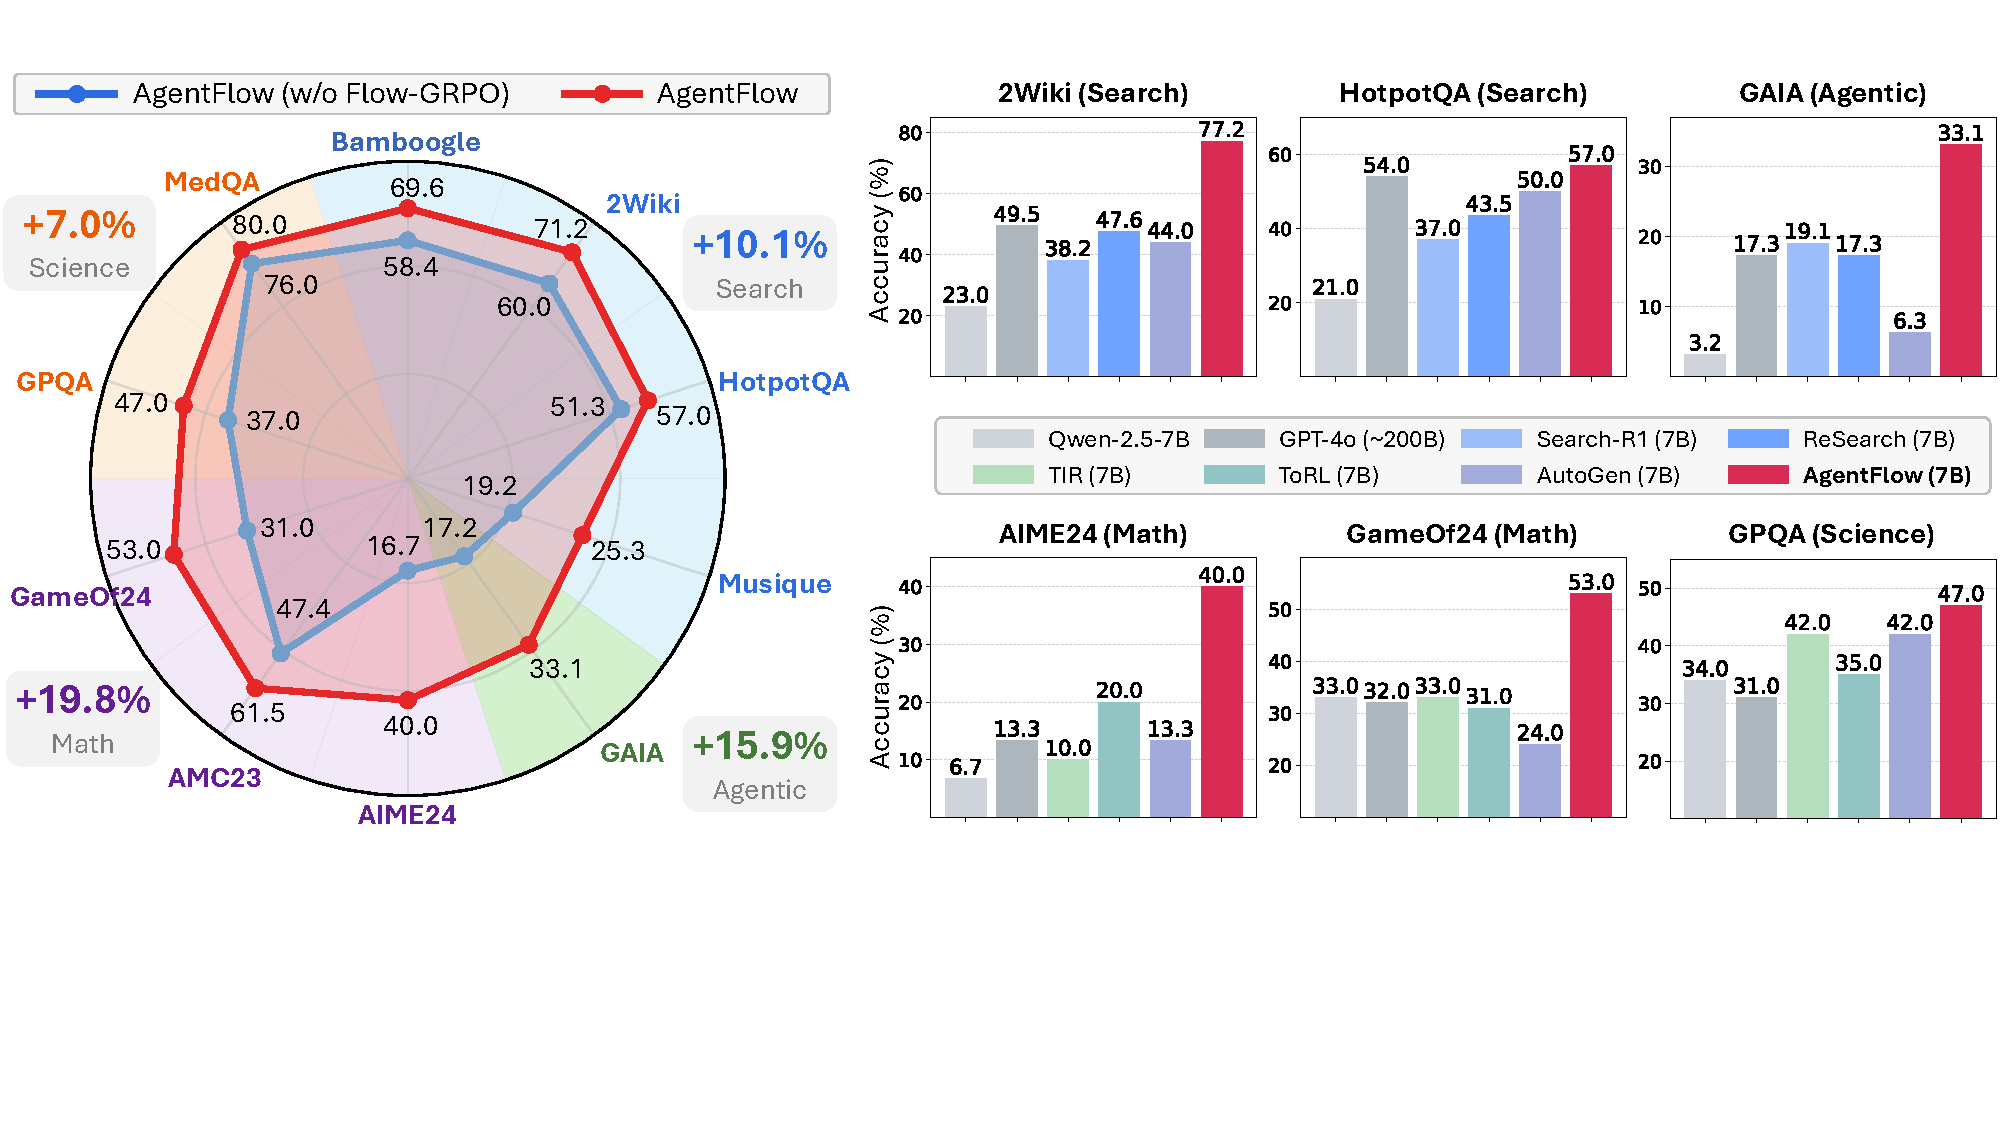
\includegraphics[width=1.0\linewidth]{figs/fig1_teaser.pdf}
    \caption{
    \textbf{Left:} Performance of \model with a 7B-scale backbone before and after Flow-GRPO tuning across ten diverse reasoning benchmarks. Flow-GRPO substantially improves performance by enhancing planning quality and tool-calling reliability.
    \textbf{Right:} \model achieves consistent gains over top baselines, including base LLMs, tool-integrated RL models, and training-free agentic systems. All 7B results use Qwen2.5-7B-Base/Instruct as the backbone and tools.}
    \label{fig:teaser_main_scores}
\end{figure}

\section{Introduction}
\vspace{-3mm}

Recent advances in large language models (LLMs) have unlocked remarkable reasoning capabilities, largely driven by reinforcement learning (RL) from outcome-based feedback. By fine-tuning models to maximize verifiable rewards, LLMs like DeepSeek-R1~\citep{guo2025deepseek} and SimpleRL~\citep{zeng2025simplerl} have demonstrated sophisticated behaviors in self-correction and multi-step deduction.

A complementary line of work augments LLMs with external tools (e.g., web search, code execution) for knowledge retrieval and precise computation. Tool-integrated reasoning (TIR) extends reinforcement learning with verifiable rewards to learn \emph{when} and \emph{how} to call tools by interleaving reasoning (e.g., \texttt{<think>}) with tool invocations (e.g., \texttt{<tool\rule[0ex]{0.5em}{0.1pt}call>}) under full context~\citep{jin2025search, song2025r1, chen2025research, feng2025retool}. Early systems supported only a single tool type, whereas recent work enables multi-tool settings by encoding tool metadata into prompts~\citep{dong2025tool, qian2025toolrl, zhang2025nemotron}. However, these methods still train a \emph{single}, monolithic policy under multi-turn full-context reasoning, which introduces scaling challenges: (i) \emph{training} becomes increasingly unstable as horizons lengthen, tool diversity grows, and environments shift with tool feedback~\citep{wang2025ragen, mai2025agent, Moonshot2025KimiResearcher, xue2025simpletir}; and (ii) \emph{inference}-time generalization remains brittle to unseen tasks or tools~\citep{dong2025tool, hu2025owl}.

Agentic systems~\citep{wu2024autogen,hong2024metagpt,hu2025owl} offer a promising alternative to monolithic tool-integrated reasoning models. They consist of multiple modules—often distinct LLMs with prescribed roles (e.g., planner, critic) or specialized components with dedicated tools and capabilities (e.g., executor, coder)—that coordinate via shared memory and inter-module communication. By decomposing problems into sub-goals and iterating over multiple turns, these systems can tackle tasks that demand diverse tools, long horizons, or multi-stage reasoning. However, achieving robust coordination in such systems ultimately requires \emph{training}, since handcrafted logic or static prompting cannot reliably capture when and how modules should collaborate, adapt to evolving tool outputs, or recover from early mistakes. At the same time, they introduce new \emph{training} challenges: modules coordinate sequentially, outcome feedback propagates through long reasoning chains, and state distributions shift with evolving tool outputs. As a result, most systems remain \emph{training-free}, relying on handcrafted logic or prompting heuristics. While some employ supervised fine-tuning or preference optimization for key modules~\citep{motwani2024malt, park2025maporl}, these off-policy approaches are decoupled from live dynamics and learn poorly from downstream successes or failures. Thus, agentic systems struggle with sparse rewards, brittle adaptation, and inefficient orchestration in dynamic environments.



To address the central challenge of learning long-horizon reasoning with sparse rewards in tool-integrated agentic systems, we introduce \model, a \emph{trainable} framework for effective planning and tool use (Figure~\ref{fig:agentflow}). \model comprises four specialized modules—planner, executor, verifier, and generator—that interact iteratively over multiple turns via a shared evolving memory and a toolset. The system operates \emph{in the flow}, with each turn cycling through planning, execution, and verification. Unlike prior agentic systems, \model directly optimizes its planner on-policy, \emph{inside} the live multi-turn loop, allowing it to dynamically adapt to trajectories shaped by tool calls, verifier signals, and memory updates. This evolving memory serves as a deterministic, structured record of the reasoning process, enabling transparent state tracking, controllable behavior, and bounded context growth.



\begin{figure}[t!]
    \centering
    \vspace{-5mm}
    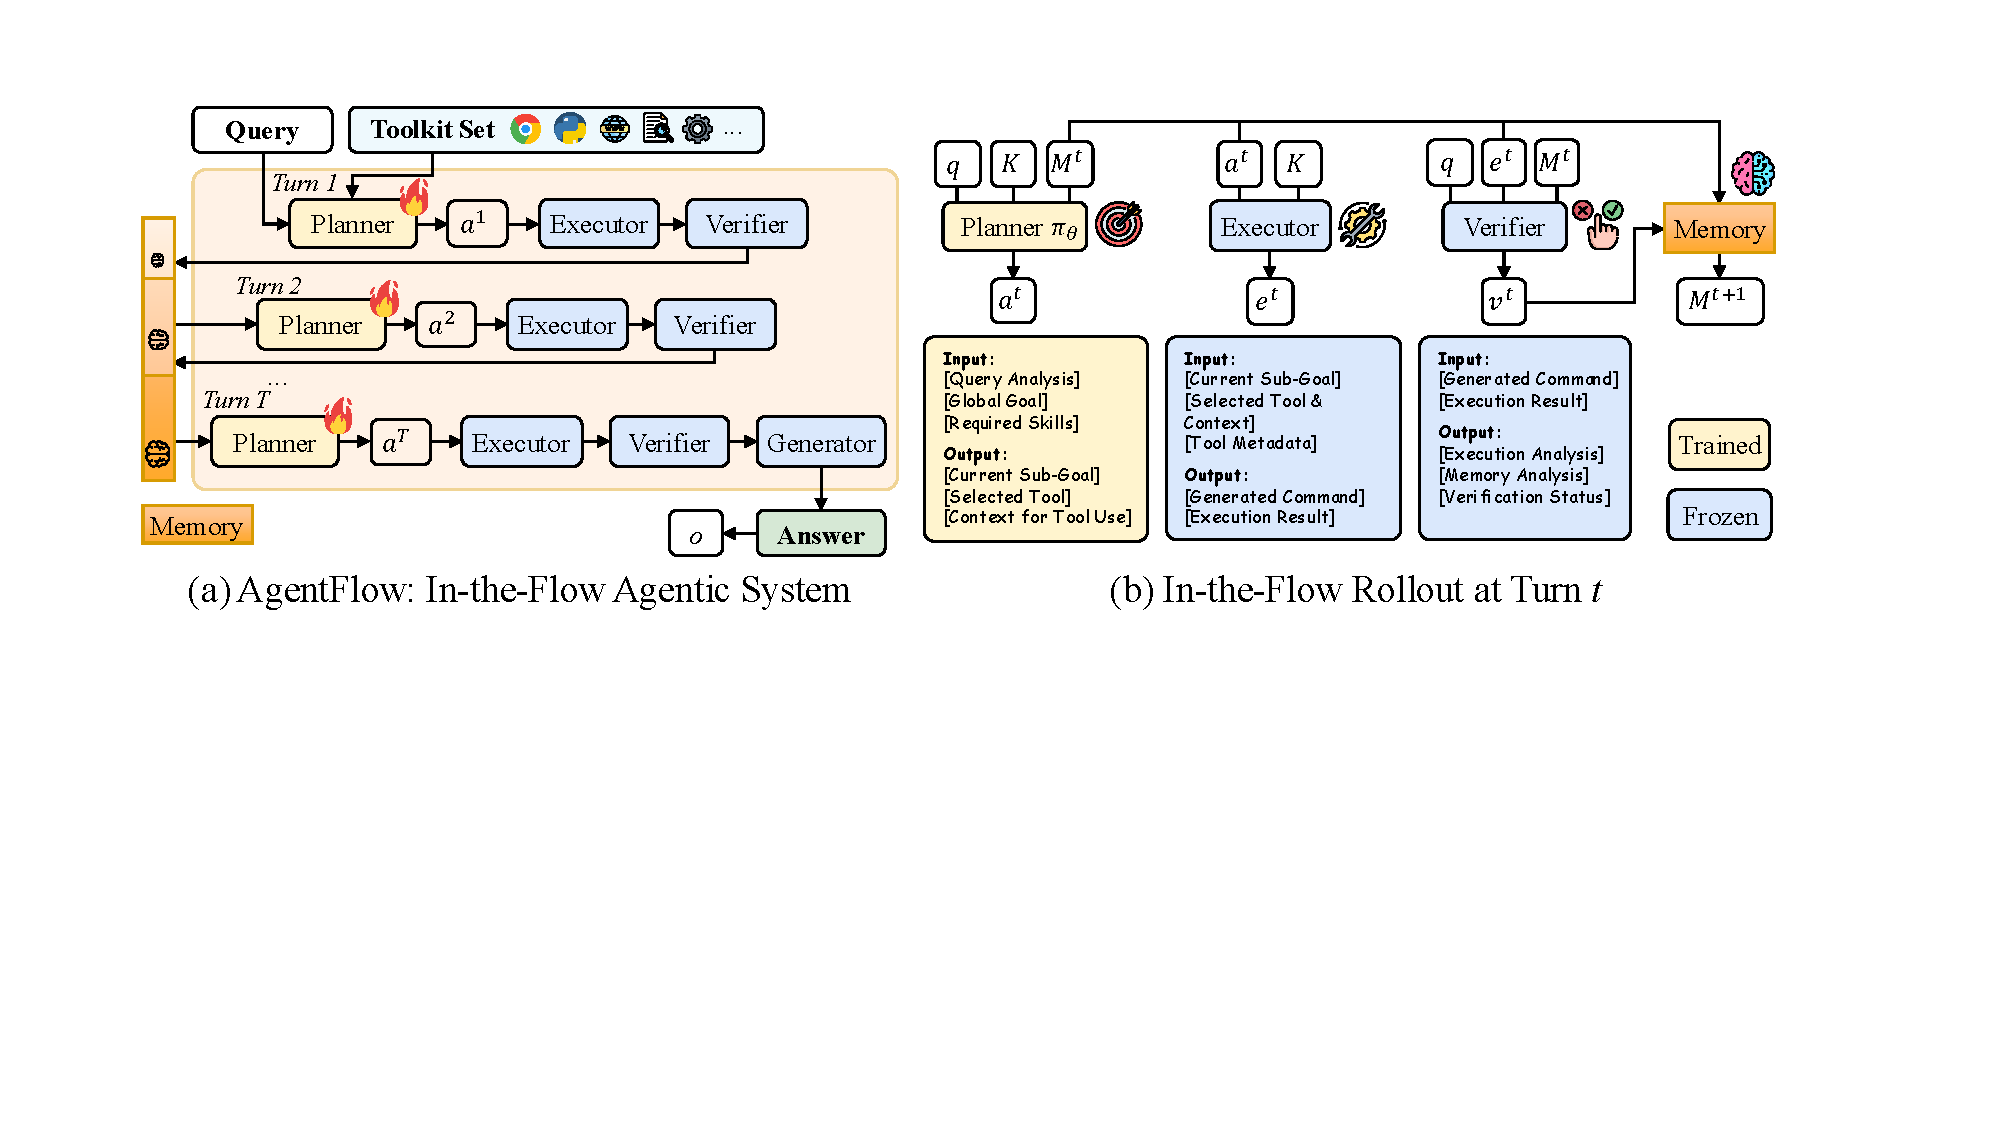
\includegraphics[width=1\linewidth]{figs/fig2_preliminary.pdf}
    \vspace{-5mm}
    \caption{\textbf{(a)} Overview of \model, a trainable agentic system for in-the-flow planning and tool use. Four modules (\text{planner}, \text{executor}, \text{verifier}, \text{generator}) coordinate via a shared evolving memory $M$ and toolset $K$, given a query $q$. The planner policy is optimized on-policy \emph{inside} the system's multi-turn loop to enable adaptive, long-horizon reasoning. \textbf{(b)} A single state transition, showing the action $a^t$, execution result $e^t$, and verifier signal $v^t$ that update the memory from $M^t$ to $M^{t+1}$.}
    \vspace{-6mm}
    \label{fig:agentflow}
\end{figure}

To train the planner on-policy within this agentic system, we need to overcome the long-horizon credit assignment problem inherent to sparse, trajectory-level rewards. We introduce \emph{Flow-based Group Refined Policy Optimization} (Flow-GRPO, Figure~\ref{fig:flow-grpo}), an on-policy algorithm designed for this setting. Flow-GRPO operates on \emph{in-the-flow} rollouts, which capture the full trajectory of states, actions, and tool events induced by the live system. Instead of attempting to assign credit with brittle, intermediate heuristics, we assign a single, verifiable final-outcome reward to the entire trajectory and \emph{broadcast} it to every turn. This design effectively transforms the multi-turn reinforcement learning challenge into a series of single-turn updates: at each turn, the planner has access to the full memory context and receives a consistent reward signal aligned with global success. This approach, coupled with group-normalized advantages to stabilize training, enables robust credit assignment and allows the planner to learn effective long-horizon strategies from sparse feedback.


We evaluate \model on ten benchmarks across diverse reasoning domains, as results highlighted in Figure~\ref{fig:teaser_main_scores}.
\model substantially outperforms top-performing specialized tool-integrated reasoning models and agentic systems, achieving average accuracy by 14.9\% on knowledge-intensive search, 14.0\% on broader agentic tasks, 14.5\% on mathematical reasoning, and 4.1\% on scientific reasoning (\S\ref{subsec:main_results}). 
Notably, our 7B-backbone system even surpasses the $\sim$200B-parameter GPT-4o ~\citep{hurst2024gpt} across all domains. Further analyses confirm that our in-the-flow optimization with Flow-GRPO is crucial, far surpassing offline supervised tuning (\S\ref{subsec:training_planner}). The trained planner learns to optimize planning, enhance tool-calling reliability, and discover effective solution pathways (\S\ref{subsec:optimized_planning}). Moreover, our training approach proves highly efficient, leading to increased rewards and condensed responses compared to traditional tool-integrated RL methods (\S\ref{subsec:traing_efficency}). Finally, we demonstrate that these benefits generalize, with consistent gains from scaling backbone size and turn budget (\S\ref{subsec:scaling_trends}).

Our work makes three key contributions: 
(1) We present \model, a trainable \emph{in-the-flow} agentic system that directly optimizes its planner \emph{inside} the multi-turn loop. By coordinating specialized modules through an evolving memory, it enables adaptive long-horizon planning and robust tool orchestration.
(2) We introduce \emph{Flow-GRPO}, an on-policy, outcome-driven algorithm that hat \emph{converts} multi-turn RL into a sequence of tractable \emph{single-turn} policy updates by \emph{broadcasting} a single, verifiable final-outcome reward to every turn.
(3) Through comprehensive experiments on ten benchmarks, we show that \model with a 7B backbone outperforms specialized baselines and even larger proprietary models. Further analyses reveal improved planning, enhanced tool-calling reliability, and positive scaling with model size and turn budgets.

\vspace{-2mm}
\section{Preliminary}
\label{sec:preliminary}
\vspace{-1mm}

\paragraph{Reinforcement learning for reasoning LLMs.}
Recent progress in reasoning LLMs has been significantly driven by reinforcement learning from outcome feedback, using a verifiable reward signal~\citep{shao2024deepseekmath, yu2025dapo}. 
This paradigm fine-tunes a language model to maximize an outcome-based reward while remaining close to a reference policy. 
Formally, the objective is to optimize a policy LLM $\pi_\theta$\textbf{} to generate a response $o$ for a given query $q$ from dataset $\mathcal{D}$:
\vspace{-1mm}
\begin{equation}
    \label{eq:rl_obj}
    \max_{\pi_\theta} \; \mathbb{E}_{q \sim \mathcal{D}, \, o \sim \pi_\theta(\cdot \mid q)} 
    \big[ R(q, o) \big] 
    - \beta \, \mathbb{D}_{\text{KL}} \!\left( \pi_\theta(o \mid q) \,\|\, \pi_{\text{ref}}(o \mid q) \right),
\end{equation}
where $R(q, o)$ is the outcome-based reward, $\pi_{\text{ref}}$ is a reference model to prevent policy collapse, and $\beta$ controls KL regularization. Algorithms like Group Relative Policy Optimization (GRPO)~\citep{shao2024deepseekmath} implement this by sampling groups of responses, normalizing advantages by their rewards, and updating the policy with a clipped objective to encourage high-reward outputs.

\begin{figure}[th!]
    \centering
    \vspace{-7mm}
    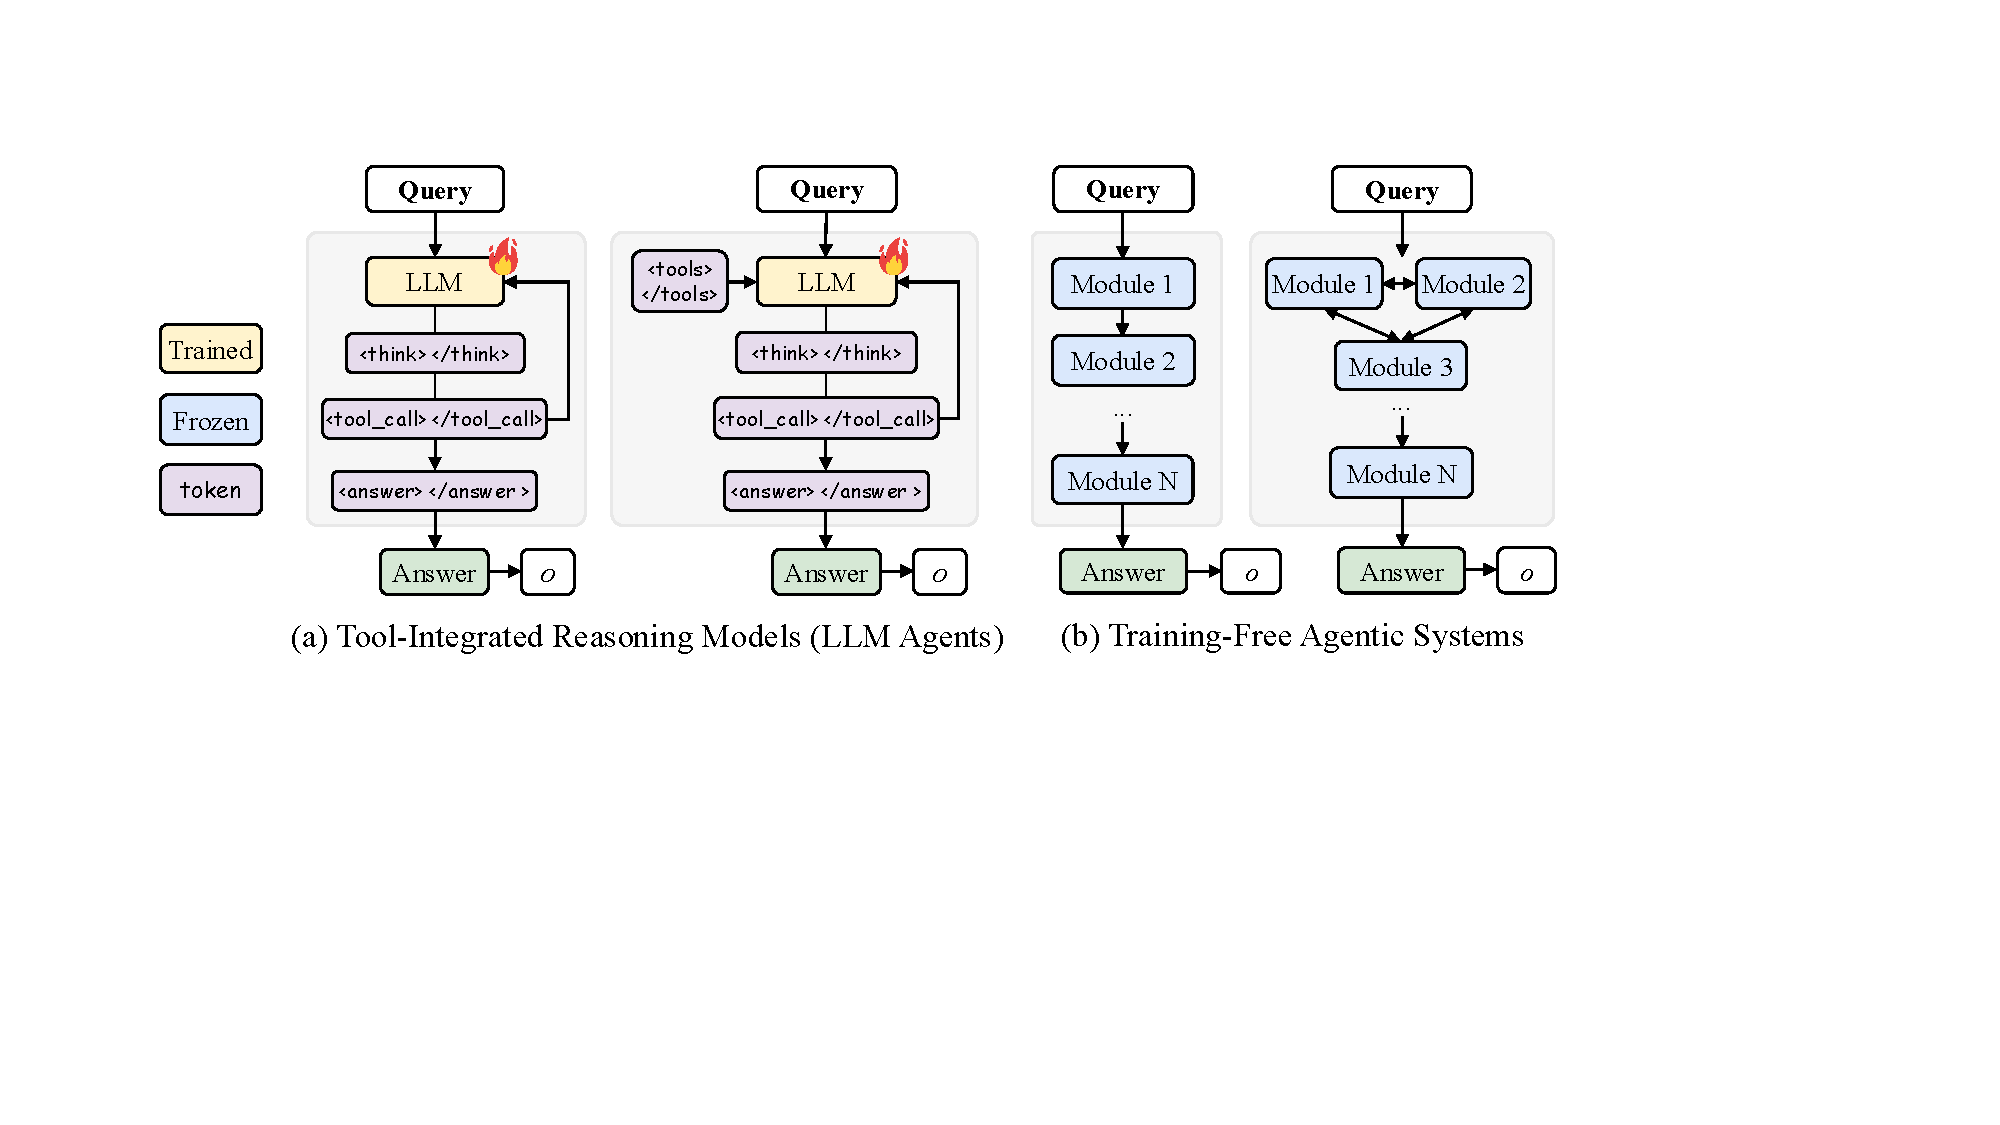
\includegraphics[width=1.0\linewidth]{figs/app_fig_preliminary.pdf}
    \vspace{-5mm}
    \caption{\textbf{Comparison of two paradigms of LLMs with tool use.} (a) Monolithic tool-integrated reasoning models train a single policy to interleave reasoning (e.g., \texttt{<think>}) and tool calls (e.g., \texttt{<tool\_call>}) within a single, full-context trajectory. (b) Agentic systems decompose tasks across multiple specialized modules (e.g., planner, coder) that collaborate. These systems are typically training-free, orchestrated by handcrafted logic or prompting.}
    \label{fig:app_preliminary}
    \vspace{-4mm}
\end{figure}

\paragraph{Tool-integrated reasoning models (LLM agents).}
LLMs can be augmented with external tools to access knowledge and perform precise computation under reinforcement learning with outcome-based reward. As shown in Figure~\ref{fig:app_preliminary}(a), the LLM \emph{interleaves} reasoning and tool calls,  producing a chain of thought within \texttt{<think></think>} tokens followed by tool invocations (e.g., \texttt{<tool\rule[0ex]{0.5em}{0.1pt}call></tool\rule[0ex]{0.5em}{0.1pt}call>}). The resulting trajectory $\tau$ is a sequence of model generations and tool observations: $\tau = \{s^1, a^1, e^1, \ldots, s^T, a^T\}$, where $s^t$ denotes the context, $a^t$ the generated action (thought + tool call), and $e^t$ the tool’s execution result. The policy model $\pi_\theta$ is then trained to maximize a final outcome reward. Prior work has explored single- and multi-tool settings for search and code execution \citep{jin2025search, chen2025research, feng2025retool, qian2025toolrl}.

\paragraph{Agentic systems with tool usage.}
An alternative approach is the use of agentic systems~\citep{wu2024autogen,hong2024metagpt,lu2025octotools}. As shown in Figure~\ref{fig:app_preliminary}(b), these frameworks deploy multiple specialized modules—often distinct LLMs with carefully designed prompts and roles—within a collaborative workflow. By decomposing tasks and assigning subproblems to modules with dedicated tools and capabilities (e.g., planner, coder, critic), they can address complex problems such as web browsing, document processing, and multi-stage programming that exceed the scope of a single model. A central limitation, however, is that these systems are typically \textit{training-free}: modules remain frozen pre-trained models orchestrated by handcrafted logic or prompting heuristics.


\vspace{-1mm}
\section{In-the-Flow Agentic System Optimization}
\label{sec:methodology}
\vspace{-1mm}

We aim to bridge the gap between trainable but monolithic reasoning models and flexible yet static agentic systems. We present \model, a flexible and trainable agentic system that integrates four specialized modules with an evolving memory (\S\ref{subsec:agentflow}). 
Unlike prior agentic systems, \model directly optimizes the planner \emph{within} the multi-turn loop of an agentic system (\S\ref{subsec:flow-grpo}).



\vspace{-1mm}
\subsection{\model: An In-the-Flow Agentic System}
\label{subsec:agentflow}


We propose \model, a general-purpose tool-integrated agentic framework for solving complex reasoning tasks through fine-grained planning and effective tool use within a multi-turn architecture. As shown in Figure~\ref{fig:agentflow}, the framework comprises four specialized modules—\textbf{Action Planner} $\mathcal{P}$, \textbf{Tool Executor} $\mathcal{E}$, \textbf{Execution Verifier} $\mathcal{V}$, and \textbf{Solution Generator} $\mathcal{G}$—coordinated by a shared evolving memory $M$ and a toolset $K$. These modules interact sequentially and iteratively to perform \emph{action planning}, \emph{tool execution}, \emph{context verification}, and \emph{solution generation}, thereby enabling tool-integrated reasoning across multiple turns.


We formalize \model's problem-solving process as a multi-turn Markov Decision Process (MDP). Given a query $q$ and a toolset $K$, the system proceeds for a variable number of turns. Let $M^t$ denote the memory state before turn $t$ (with $M^1$ initialized from $q$). At turn $t$, the planner $\mathcal{P}$ (a trainable policy $\pi_\theta$) formulates a sub-goal, selects an appropriate tool $k \in K$, and retrieves relevant context from memory, producing an action: $a^t \sim \pi_\theta(a^t \mid q, K, M^t)$.


The executor $\mathcal{E}$ invokes the chosen tool with context, yielding an execution observation $e^t \sim \mathcal{E}(e^t \mid a^t, K)$.
The verifier $\mathcal{V}$ then evaluates whether $e^t$ is valid and whether the accumulated memory is sufficient to solve the query, producing a binary verification signal $v^t \sim \mathcal{V}(v^t \mid q, e^t, M^t)$.
If $v^t = 0$, the memory is updated deterministically to incorporate new evidence: $M^{t+1} = f_{\text{mem}}\!(M^t, a^t, e^t, v^t)$,
where $f_{\text{mem}}(\cdot)$ denotes the memory-update function, which records agent-process information in a concise, structured form along with contextual details such as time, turn index, and error signals.

The process repeats until $v^t = 1$ (termination) or a predefined maximum turn budget is reached. Upon termination at turn $T$, the solution generator $\mathcal{G}$ produces the final solution $o$, conditioned on the query and the accumulated memory: $o \sim \mathcal{G}(o \mid q, M^T)$.

This formulation decomposes multi-turn, tool-integrated reasoning into structured, observable transitions. After $T$ turns, the trajectory $\tau = \{(a^t, e^t, v^t)\}_{t=1}^T$ records the history of planning, execution, and verification. The joint generative process can be written as
\vspace{-1mm}
{\small
\begin{equation}
    \label{eq:joint_policy}
    p_\theta\!\left(\{a^t, e^t, v^t\}_{t=1}^T,\, o \mid q, K\right)
    = \Bigg[\prod_{t=1}^T \pi_\theta(a^t \mid q, K, M^t)\;
      \mathcal{E}(e^t \mid a^t, K)\;
      \mathcal{V}(v^t \mid q, e^t, M^t)\Bigg]\;
      \mathcal{G}(o \mid q, M^T),
\end{equation}
}where $\{a^t, e^t, v^t\}_{t=1}^T$ are explicit realizations of the latent reasoning chain. Importantly, unlike latent thoughts behind trajectories, our memory $M$ is an explicit and deterministic record of the reasoning process, ensuring transparency and controllability of multi-turn decisions.

\begin{figure}[t!]
    \centering
    \vspace{-2mm}
    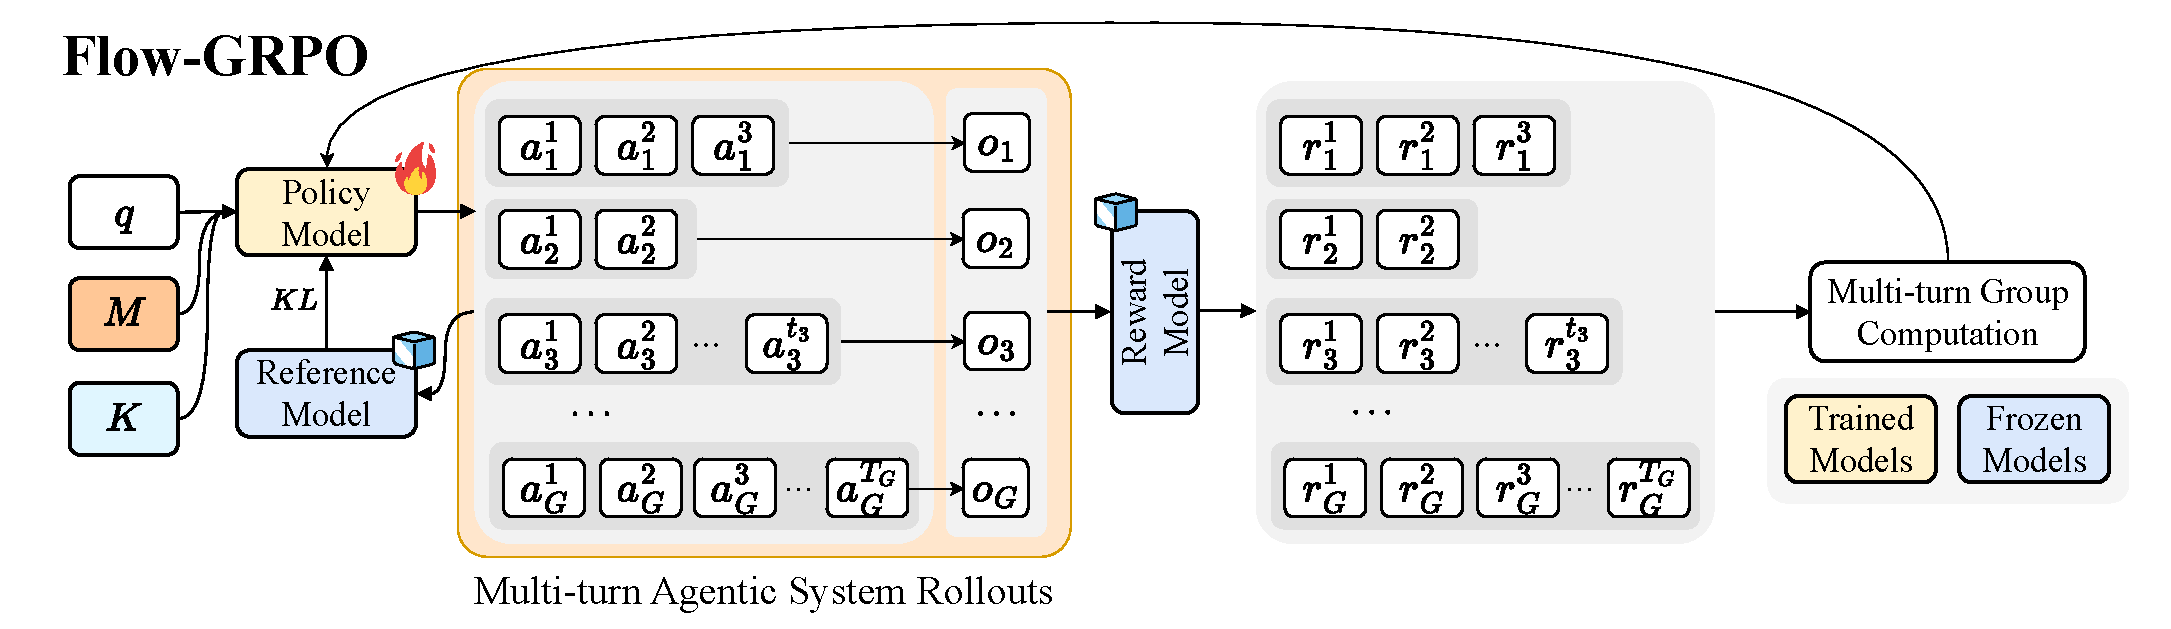
\includegraphics[width=0.95\linewidth]{figs/fig3_method.pdf}
    \vspace{-2mm}
    \caption{\textbf{Optimization for our proposed agentic system \model.} Given a query $q$, an evolving memory $M$, and a toolset $K$, the policy model generates actions that target sub-goals and select tools. It is trained via \textit{Flow-based Group Refined Policy Optimization} (Flow-GRPO), which enables multi-turn reinforcement learning and stable optimization under collaborative dynamics.}
    \vspace{-4mm}
    \label{fig:flow-grpo}
\end{figure}

\vspace{-1mm}
\subsection{In-The-Flow Reinforcement Learning Optimization}
\label{subsec:flow-grpo}
 
We target tool-integrated \emph{agentic systems} operating under \emph{long-horizon} tasks with \emph{sparse} rewards. In this setting, the \textbf{Action Planner} (the trainable policy of \model) selects a \emph{sequence} of interdependent actions while the state $(q, K, M^t)$ evolves with tool results and verifier feedback. Conventional \textit{offline} training—e.g., supervised fine-tuning or preference fine-tuning on curated traces—optimizes the planner \emph{outside} the active loop~\citep{motwani2024malt, park2025maporl}. This decoupling prevents real-time coordination with the executor, verifier, and solution generator, induces distribution shift between training and deployment, and provides limited guidance about \emph{which} intermediate decisions truly matter. As a result, planners often adapt poorly to multi-turn dynamics; early errors cascade, and post-hoc fixes are brittle.

\paragraph{In-the-flow learning.}
To address these issues, we optimize the planner \emph{in the flow} of execution. We roll out the full \model system under the current policy, collect the actual trajectory $\tau$ of states, actions, and tool events it induces, and update the policy within the agentic system using a verifiable final-outcome signal. This exposes the multi-turn credit-assignment problem directly and trains the planner on the exact states it will face at inference. Our objective, Flow-GRPO, is designed to stabilize learning under sparse, trajectory-level rewards over multiple turns.

As established in \S\ref{subsec:agentflow}, rollouts in \model define a finite-horizon MDP with a variable horizon $T$. At turn $t$, the planner observes the state $(q, K, M^t)$, selects an action $a^t$, the executor and verifier return $(e^t, v^t)$, and the memory updates deterministically to $M^{t+1}$.

\paragraph{Policy optimization objective.}
The planner policy $\pi_\theta$ is trained to maximize the expected return over on-policy rollouts. Let $R(\tau)$ be the reward for a complete trajectory $\tau$. The objective is:
\begin{equation}
    \mathcal{J}(\theta)=\mathbb{E}_{\tau\sim\pi_\theta}\!\big[R(\tau)\big], \qquad \theta^\star=\arg\max_\theta \mathcal{J}(\theta),
\end{equation}
where a rollout $\tau$ is the sequence of decisions $\{a^t\}_{t=1}^{T}$  generated on-policy by $\pi_\theta$.


\paragraph{Final-outcome reward.}
Assigning credit to intermediate actions is challenging because each $a^t$ influences the final solution only indirectly, and their value may only emerge after several turns (e.g., error or improvement accumulation). To avoid brittle local feedback, we adopt a \emph{final-outcome-based reward}: every action within a rollout receives the same global reward signal, based on the correctness of the final solution $o$ with respect to query $q$ and ground truth $y^*$:
\begin{align}
    r = R(a^t) = \bar{R}(o, q, y^*), \quad \forall t = 1,\dots,T,
    \label{eq:reward_func}
\end{align}
where $\bar{R}(o, q, y^*) \in \{0, 1\}$ is assigned by an LLM-as-judge rubric for semantic, numeric, and option-level equivalence (see \S\ref{app:llm_based_judging}). This propagates a trajectory-level success signal back through the reasoning chain, aligning every decision $a^t$ with global correctness.

\paragraph{Objective function.} 
We formalize \textbf{Flow}-based \textbf{G}roup \textbf{R}efined \textbf{P}olicy \textbf{O}ptimization for the planner. The goal is to optimize the policy $\pi_\theta$ by maximizing the expected return over a group of parallel rollouts. For each query-label pair from training corpus $(q,y^*) \sim \mathcal{D}$, we sample a group of $G$ on-policy trajectories $\{\tau_i\}_{i=1}^G$ by running the current behavior policy $\pi_{\theta_\text{old}}$ inside \model, where $\tau_i = \{a_i^1, ....a_i^{T_i}, o_i\}$. Let $s_i^t=(q, K, M_i^t)$ be the state at turn $t$ of rollout $i$, $a_i^t$ the planner’s action (a token sequence of length $|a_i^t|$), and $o_i$ the final response. 
This structure is key to addressing the long-horizon credit assignment challenge: by broadcasting a single trajectory-level reward to all turns, we effectively decompose the \emph{multi-turn RL} problem into \emph{a set of independent, single-turn} policy updates; we provide a formal proof of this equivalence and analyze its convergence properties in \S\ref{app:mathematical_analysis}. Each update for an action $a_i^t$ is conditioned on the full historical context encapsulated in the state $s_i^t$ and receives the same global success signal, simplifying optimization. 
The objective is
{\small
\begin{equation}
    \label{eq:Flow-GRPO_objective}
    \begin{aligned}
    \mathcal{J}_{\text{Flow-GRPO}}(\theta) &= \mathbb{E}_{(q, y^*) \sim \mathcal{D}, \; \{\tau_i\}_{i=1}^{G} \sim \pi_{\theta_\text{old}}}  \\
    & \Bigg[
    \frac{1}{G}\sum_{i=1}^{G}\frac{1}{T_i}\sum_{t=1}^{T_i}\frac{1}{|a_i^t|}\sum_{j=1}^{|a_i^t|}
    \min\!\Big\{ \rho_{i,j}^t A_i^t,\, \mathrm{clip}(\rho_{i,j}^t,\,1-\epsilon,\,1+\epsilon)\,A_i^t \Big\}
    \;-\; \beta\, \mathbb{D}_{\mathrm{KL}}\!\big(\pi_\theta \,\|\, \pi_{\text{ref}}\big)
    \Bigg],
    \end{aligned}
\end{equation}
}where $T_i$ is the (variable) number of turns in rollout $i$, and
\begin{equation}
    \label{eq:ratio_def}
    \rho_{i,j}^t
    = \frac{\pi_\theta\!\big(a_{i,j}^t \,\big|\, s_i^t, a_{i,1:j-1}^t\big)}
    {\pi_{\theta_\text{old}}\!\big(a_{i,j}^t \,\big|\, s_i^t, a_{i,1:j-1}^t\big)}
\end{equation}
is the token-level importance ratio for the $j$-th token of $a_i^t$, $\epsilon>0$ is the PPO clipping parameter, and $\beta>0$ controls the KL penalty to a fixed reference policy $\pi_{\text{ref}}$.

\paragraph{Group-normalized advantages.}
Because the reward in Eq.~\ref{eq:reward_func} is a single trajectory-level signal, the per-turn advantage $A_i^t$ is constant over $t$ within a rollout $i$. We reduce variance and sharpen credit assignment across the group by using a \emph{group-normalized} advantage:
\vspace{-1mm}
\begin{equation}
    \label{eq:advantage_norm}
    A_i^t = \frac{\bar{R}(o_i, q, y^*) - \mathrm{mean}\left( \{ \bar{R}(o_k, q, y^*) \}_{k=1}^{G} \right)}{\mathrm{std}\left( \{ \bar{R}(o_k, q, y^*) \}_{k=1}^{G} \right)}.
\end{equation}





\section{Experiments}
\label{sec:experiments}
\vspace{-1mm}

\subsection{Experimental Setup}
\label{subsection:exp_setup}



In our main experiments, all modules—{Action Planner}, {Tool Executor}, {Executive Verifier}, and {Solution Generator}—are instantiated with the \textit{Qwen2.5-7B-Instruct} model~\citep{yang2024qwen2.5}. Among these, only the \textit{Action Planner} is trainable. The system operates with five interactive tools: \textit{Base Generator} is an instance of \textit{Qwen2.5-7B-Instruct} that acts as the default reasoning engine if the planner decides not to use an external tool; \textit{Python Coder} generates and executes Python code given a query and returns the execution result; \textit{Google Search} searches the web and returns a summarization of Top-K search results; \textit{Wikipedia Search} searches articles matching a given query and returns a summarization; and \textit{Web Search} returns summarized information from a given web page. During the RL fine-tuning phase, we mix data from Search-R1~\citep{jin2025search} and DeepMath~\citep{he2025deepmath} as training data, which provides paired question-answer examples across search and mathematical domains. We use a batch size of 32 with 8 rollouts per sample.


\begin{table}[t!]
    \vspace{-1mm}
    \centering
    \footnotesize
    \setlength{\tabcolsep}{0.5em}
    \renewcommand{\arraystretch}{0.95}
    \resizebox{\textwidth}{!}{
    \begin{tabular}{ll|cccc|cc|cc}
    \toprule
    \multirow{2}{*}{} & \multirow{2}{*}{} & \multicolumn{6}{c}{\cellcolor{SearchBg}\textbf{Search Intensive}} & \multicolumn{2}{c}{\cellcolor{AgenticBg}\textbf{Agentic}} \\
    \cmidrule(lr){3-8} \cmidrule(lr){9-10}
    \textbf{Model} & \textbf{Size} & \textbf{Bamboogle} & \textbf{2Wiki} & \textbf{HotpotQA} & \textbf{Musique} & \textbf{~Avg.~} & \textbf{$\Delta$} & \textbf{GAIA} & \textbf{$\Delta$} \\
    \midrule
    Qwen-2.5-7B-Instruct & 7B-Inst & 12.0 & 23.0 & 21.0 & 6.0 & 15.5 & \mygreen{83.6}\gain{41.8} & 3.2 & \mygreen{59.8}\gain{29.9} \\
    Qwen-2.5-14B-Instruct & 14B-Inst & 21.6 & \underline{26.7} & 20.0 & 8.0 & 19.1 & \mygreen{76.4}\gain{38.2} & 5.5 & \mygreen{55.2}\gain{27.6} \\
    Qwen-2.5-32B-Instruct & 32B-Inst & \underline{24.0} & \underline{26.7} & 27.0 & 6.0 & 20.9 & \mygreen{72.8}\gain{36.4} & \underline{9.5} & \mygreen{47.2}\gain{23.6} \\
    Llama-3.3-70B-Instruct & 70B-Inst & 18.4 & 22.7 & \underline{52.0} & \underline{16.0} & \underline{27.3} & \mygreen{60.0}\gain{30.0} & 3.2 & \mygreen{59.8}\gain{29.9} \\
    \midrule
    GPT-4o-mini~\citep{hurst2024gpt} & $\sim$8B & 40.8 & 35.6 & 41.0 & 15.0 & 33.1 & \mygreen{48.4}\gain{24.2} & 7.1 & \mygreen{52.0}\gain{26.0} \\
    GPT-4o~\citep{hurst2024gpt} & $\sim$200B & \underline{68.8} & \underline{49.5} & \underline{54.0} & \underline{24.0} & \underline{49.1} & \mygreen{16.4}\gain{8.2} & \underline{17.3} & \mygreen{31.6}\gain{15.8} \\
    \midrule
    Supervised Fine-Tuning (SFT) & 7B-Inst & 12.0 & 25.9 & 22.0 & 6.6 & 16.6 & \mygreen{83.6}\gain{40.7} & 3.2 & \mygreen{59.8}\gain{29.9} \\
    \midrule
    Iter-RetGen~\citep{shao2023enhancing} & 7B-Inst & 36.8 & 33.6 & 37.4 & 17.8 & 31.4 & \mygreen{51.8}\gain{25.9} & 3.9 & \mygreen{58.4}\gain{29.2} \\
    Search-R1~\citep{jin2025search} & 7B-Inst & 43.2 & 38.2 & 37.0 & 14.6 & 33.3 & \mygreen{48.0}\gain{24.0} & \underline{19.1} & \mygreen{28.0}\gain{14.0} \\
    ZeroSearch~\citep{sun2025zerosearch} & 7B-Base & 27.8 & 35.2 & 34.6 & 18.0 & 28.9 & \mygreen{56.8}\gain{28.4} & 16.5 & \mygreen{33.2}\gain{16.6} \\
    ReSearch~\citep{chen2025research} & 7B-Base & 42.4 & \underline{47.6} & 43.5 & 22.3 & \underline{39.0} & \mygreen{36.6}\gain{18.3} & 17.3 & \mygreen{31.6}\gain{15.8} \\
    StepSearch~\citep{wang2025stepsearch} & 7B-Base & 40.0 & 36.6 & 38.6 & \underline{22.6} & 34.5 & \mygreen{45.6}\gain{22.8} & -- & -- \\
    VerlTool~\citep{jiang2025verltool} & 7B-Base & \underline{46.4} & 45.3 & \underline{44.8} & 19.3 & \underline{39.0} & \mygreen{36.6}\gain{18.3} & 11.2 & \mygreen{43.8}\gain{21.9} \\
    \midrule
    AutoGen~\citep{wu2024autogen} & 7B-Inst & 59.6 & 44.0 & 50.0 & 15.9 & 42.4 & \mygreen{29.8}\gain{14.9} & 6.3 & \mygreen{53.6}\gain{26.8} \\
    \midrule
    \textbf{\model} & 7B-Inst & 58.4 & 60.0 & 51.3 & 19.2 & 47.2 & \mygreen{26.8}\gain{12.1} & 17.2 & \mygreen{31.8}\gain{15.9} \\
    \textbf{\model} (w/ Flow-GRPO) & 7B-Inst & \textbf{69.6} & \textbf{77.2} & \textbf{57.0}& \textbf{25.3} & \textbf{57.3} & -- & \textbf{33.1} & -- \\
    \bottomrule
    \end{tabular}
    } %
    \vspace{-2mm}
    \caption{\textbf{Accuracy comparison on search-intensive and agentic tasks.} 7B-Base refers to Qwen-2.5-7B-Base and 7B-Inst refers to Qwen-2.5-7B-Instruct. AutoGen and our \model method are agentic systems, which use Qwen-2.5-7B-Instruct for the LLM-powered agents and tools for fair comparison. 
    We visualize the gains of \model to the each baseline in the \colorbox{DeltaBg}{$\Delta$ columns}.}
    \vspace{-2mm}
    \label{tab:main_table_search_agentic}
\end{table}



\begin{table}[t!]
    \centering
    \footnotesize
    \setlength{\tabcolsep}{0.3em}
    \renewcommand{\arraystretch}{0.95}
    \resizebox{\textwidth}{!}{
    \begin{tabular}{ll|ccc|cc|cc|cc}
    \toprule
    \multirow{2}{*}{} & \multirow{2}{*}{} & \multicolumn{5}{c}{\cellcolor{MathBg}\textbf{Math Reasoning}} & \multicolumn{4}{c}{\cellcolor{ScienceBg}\textbf{Scientific Reasoning}}  \\
    \cmidrule(lr){3-7} \cmidrule(lr){8-11}
    \textbf{Model} & \textbf{Size} & \textbf{AIME24} & \textbf{AMC23} & \textbf{GameOf24} & \textbf{~Avg.~} & \textbf{$\Delta$} & \textbf{GPQA} & \textbf{MedQA} & \textbf{~Avg.~} & \textbf{$\Delta$} \\
    \midrule
    Qwen-2.5-7B-Instruct & 7B-Inst & 6.7 & 47.5 & \underline{33.0} & 29.1 & \mygreen{67.5}\gain{22.5} & 34.0 & 66.0 & 50.0 & \mygreen{40.5}\gain{13.5} \\
    Qwen-2.5-14B-Instruct & 14B-Inst & 6.7 & \underline{60.0} & 25.0 & 30.6 & \mygreen{63.0}\gain{21.0} & 31.0 & \underline{75.0} & \underline{53.0} & \mygreen{31.5}\gain{10.5} \\
    Llama-3.3-70B-Instruct & 70B-Inst & 6.7 & 47.5 & 31.0 & 28.4 & \mygreen{69.3}\gain{23.1} & \underline{35.0} & 67.0 & 51.0 & \mygreen{37.5}\gain{12.5} \\
    Llama-3.1-405B-Instruct & 405B-Inst & \underline{26.7} & 47.5 & 23.0 & \underline{32.4} & \mygreen{57.3}\gain{19.1} & 30.0 & 62.0 & 46.0 & \mygreen{52.5}\gain{17.5} \\
    \midrule
    GPT-4o-mini~\citep{hurst2024gpt} & $\sim$8B & \underline{13.3} & 57.5 & 16.0 & 28.9 & \mygreen{67.8}\gain{22.6} & 27.0 & \underline{66.0} & \underline{46.5} & \mygreen{51.0}\gain{17.0} \\
    GPT-4o~\citep{hurst2024gpt} & $\sim$200B & \underline{13.3} & \underline{60.0} & \underline{32.0} & \underline{35.1} & \mygreen{49.2}\gain{16.4} & \underline{31.0} & 60.0 & 45.5 & \mygreen{54.0}\gain{18.0} \\
    \midrule
    Supervised Fine-Tuning (SFT) & 7B-Inst & 6.7 & 47.5 & \underline{33.0} & 29.1 & \mygreen{67.5}\gain{22.5} & 34.0 & 66.0 & 50.0 & \mygreen{40.5}\gain{13.5} \\
    \midrule
    SimpleRL-reason~\citep{zeng2025simplerl} & 7B-Base & 16.7 & \underline{60.0} & \underline{33.0} & \underline{36.6} & \mygreen{45.0}\gain{15.0} & \underline{45.0} & 65.0 & 50.0 & \mygreen{40.5}\gain{13.5} \\
    Open-Reasoner-Zero~\citep{hu2025open} & 7B-Base & 16.7 & 54.9 & 32.0 & 34.5 & \mygreen{51.0}\gain{17.0} & 34.0 & 54.0 & 44.0 & \mygreen{58.5}\gain{19.5} \\
    General-Reasoner~\citep{ma2025general} & 7B-Base & 13.3 & 55.0 & \underline{33.0} & 33.8 & \mygreen{53.1}\gain{17.7} & 35.5 & 61.0 & 48.3 & \mygreen{45.6}\gain{15.2} \\
    Luffy~\citep{yan2025learning} & 7B-Inst & \underline{30.7} & 44.8  & \underline{33.0} & 36.2 & \mygreen{45.9}\gain{15.3} & 34.0 & \underline{77.0} & \underline{55.5} & \mygreen{24.0}\gain{8.0} \\
    \midrule
    TIR~\citep{yang2024qwen2} & 7B-Inst & 10.0 & 50.0 & \underline{33.0} & 31.0 & \mygreen{61.5}\gain{20.5} & \underline{42.0} & \underline{76.8}  & \underline{59.4} & \mygreen{12.3}\gain{4.1} \\
    ToRL~\citep{li2025torl} & 7B-Inst & \underline{20.0} & \underline{60.0} & 31.0 & \underline{37.0} & \mygreen{46.8}\gain{14.5} & 35.0 & 76.5 & 55.8 & \mygreen{24.1}\gain{7.7} \\
    \midrule
    AutoGen~\citep{wu2024autogen} & 7B-Inst & 13.3 & 57.5 & 24.0 & 31.6 & \mygreen{59.7}\gain{19.9} & 42.0 & 72.0 & 57.0 & \mygreen{19.5}\gain{6.5} \\
    \midrule
    \textbf{\model} & 7B-Inst & 16.7 & 47.4 & 31.0 & 31.7 & \mygreen{59.4}\gain{19.8} & 37.0 & 76.0 & 56.5 & \mygreen{21.0}\gain{7.0} \\
    \textbf{\model} (w/ Flow-GRPO) & 7B-Inst & \textbf{40.0} & \textbf{61.5} & \textbf{53.0} & \textbf{51.5} & -- & \textbf{47.0} & \textbf{80.0} & \textbf{63.5} & -- \\
    \bottomrule
    \end{tabular}
    } %
    \vspace{-3mm}
    \caption{\textbf{Accuracy comparison of mathematical and scientific reasoning tasks.}} 
    \label{tab:main_table_math_science}
    \vspace{-5mm}
\end{table}


To comprehensively evaluate tool-use capabilities of \model, we conduct experiments on four types of reasoning tasks: (1) \textit{Knowledge-intensive search} including Bamboogle~\citep{press2023measuring}, 2Wiki~\citep{ho2020constructing}, HotpotQA~\citep{yang2018hotpotqa}, and Musique~\citep{trivedi2022musique}; (2) \textit{Agentic reasoning} such as GAIA~\citep{mialon2023gaia} (where we adopt the textual split); (3) \textit{Logic-dense mathematical reasoning} including AIME2024~\citep{aops_aime}, AMC23~\citep{AMC23}, and GameOf24~\citep{lightman2023let}; and (4) \textit{Scientific reasoning} including GPQA~\citep{rein2024gpqa} and MedQA~\citep{yang2024llm}. To mitigate randomness, we report the average accuracy across three trials for all experiments. More experimental details are in \S\ref{app:exp_details}.

\subsection{Main Results}
\label{subsec:main_results}

\paragraph{Baselines.} As presented in Tables \ref{tab:main_table_search_agentic} and \ref{tab:main_table_math_science}, we include five categories of baselines: 
(1) \textit{Open-source LLMs}: Qwen2.5~\citep{yang2024qwen2.5}, Llama-3.1, and Llama-3.3~\citep{dubey2024llama}; 
(2) \textit{Proprietary LLMs}: GPT-4o-mini and GPT-4o;
(3) \textit{Reasoning LLMs}: supervised fine-tuning~\citep{yang2024qwen2}, SimpleRL-reason, Open-Reasoner-Zero, General-Reasoner, and LUFFY; (4) \textit{Tool-integrated reasoning LLMs}: both search-enhanced, including Iter-RetGen, Search-R1, ZeroSearch, ReSearch, StepSearch, and VerlTool, and code-enhanced, including TIR and ToRL; (5) \textit{Training-free agentic system}: AutoGen. More details on baseline implementations are in \S\ref{app:baseline}.

\paragraph{Key insights.}
\model consistently outperforms all baseline models by large margins. Compared to the best-performing 7B models without tool integration, \model achieves absolute gains of 40.7\% on search (SFT), 29.9\% on agentic reasoning (SFT), 15.0\% on math (SimpleRL-reason), and 8.0\% on scientific tasks (Luffy). Against specialized tool-integrated systems, \model surpasses the top models by 14.9\% in search (AutoGen), 14.0\% in agentic reasoning (Search-R1), 14.5\% in math (ToRL), and 4.1\% in science (TIR). Notably, our 7B-backbone \model even outperforms the $\sim$200B-parameter GPT-4o across all domains, with gains ranging from 8.2\% to 18.0\%. A detailed analysis is provided in \S\ref{app:main_result_analysis}.


\begin{figure}[t!]
    \centering
    \vspace{-5mm}
    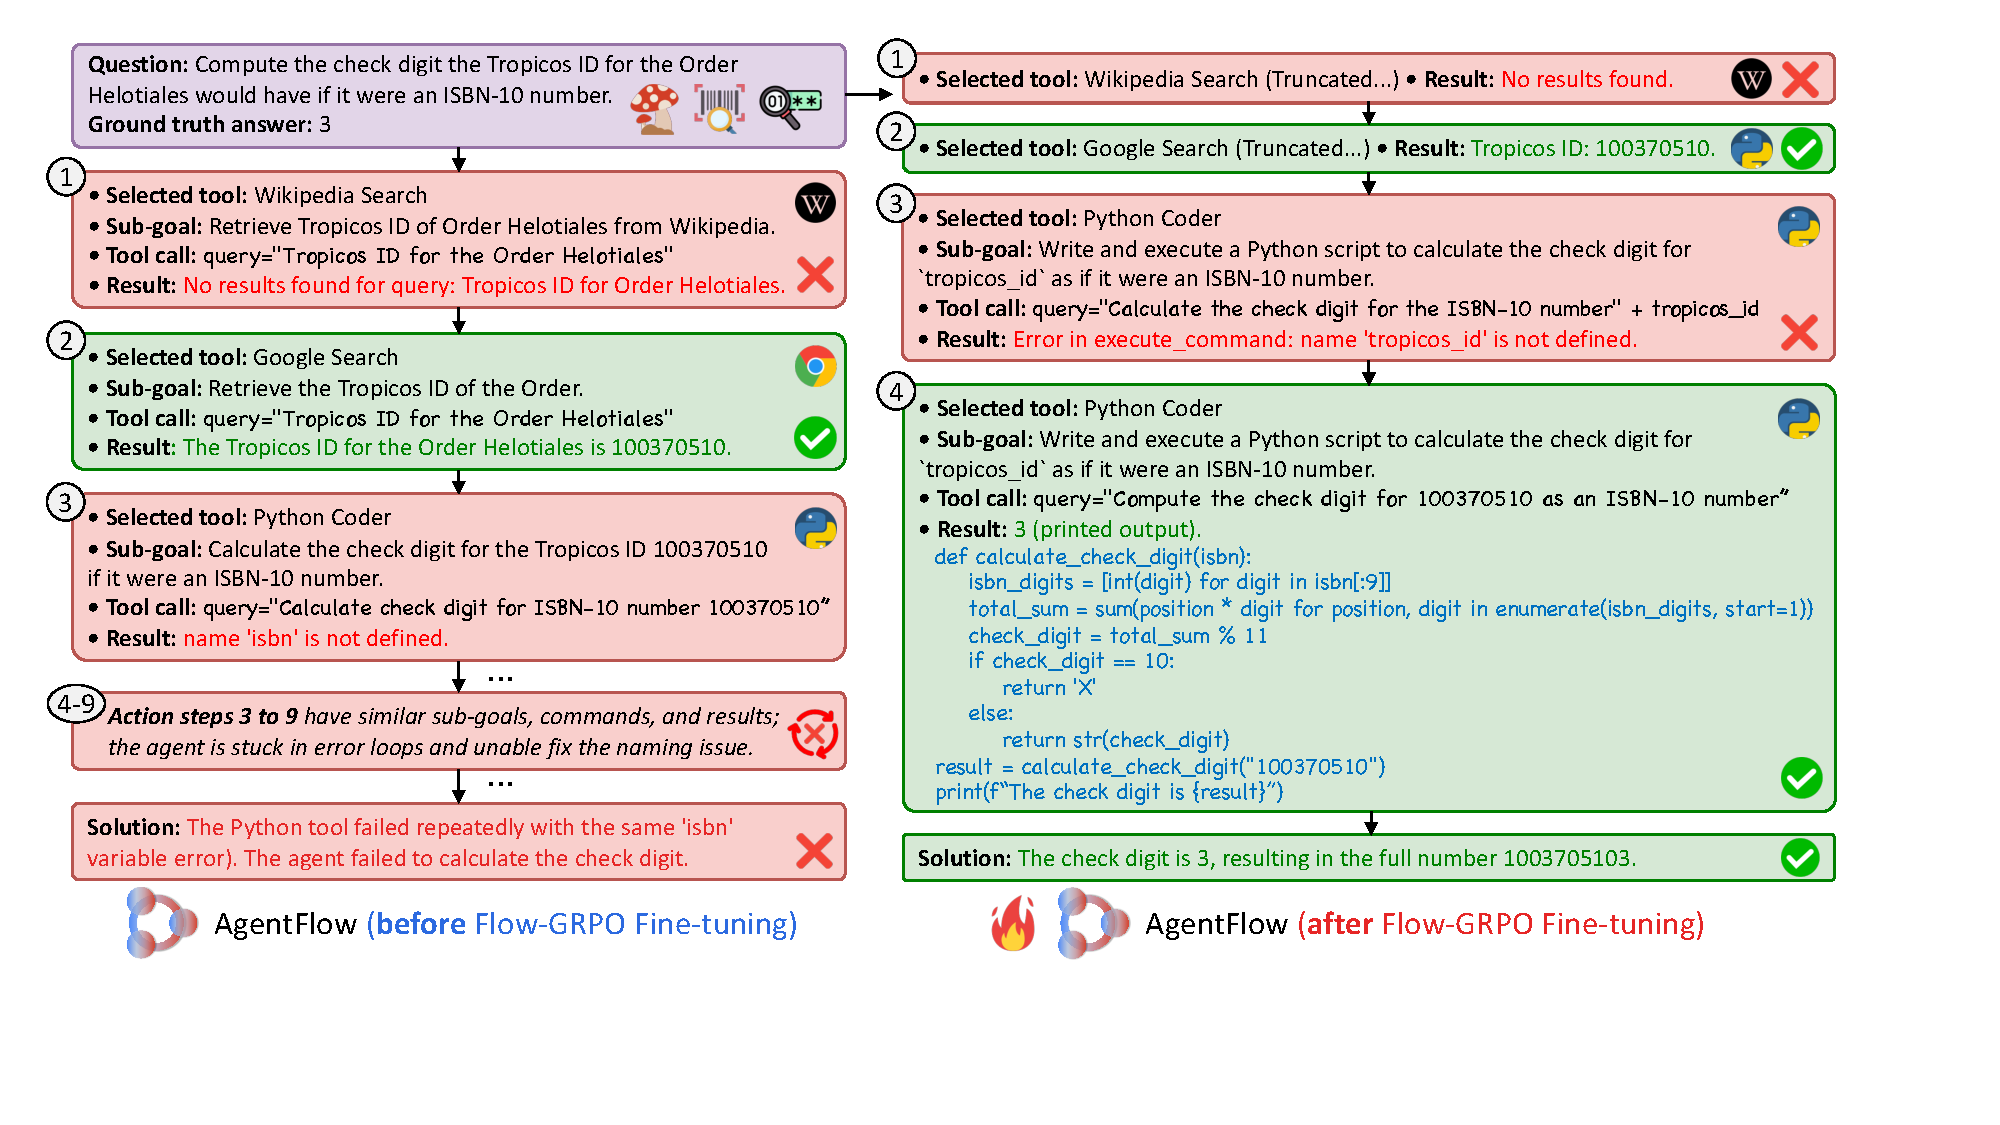
\includegraphics[width=1.0\linewidth]{figs/fig_case_study.pdf}
    \vspace{-6mm}
    \caption{\textbf{One case study example.} Initially failed with repetitive errors (left), \model, trained with Flow-GRPO, explores a new solution pathway at turn 4 after two failed attempts (right).}
    \vspace{-3mm}
    \label{fig:fig_case_study}
\end{figure}


\subsection{Training Strategies on the Planner}
\label{subsec:training_planner}

We conduct an ablation study to analyze the impact of different training strategies for the \textit{Action Planner} module in \model, with results reported in Table~\ref{tab:individual_vs_inflow}. The executor, verifier, and generator modules remain fixed as Qwen2.5-7B-Instruct, consistent with our main setup (\S\ref{subsection:exp_setup}).


\begin{table}[htbp]
  \centering
  \vspace{-2mm}
  \setlength{\tabcolsep}{0.4em}
  \resizebox{0.95\textwidth}{!}{
  \begin{tabular}{llllllllll}
  \toprule
  \textbf{Planner Model} & \textbf{Training} & \textbf{Bamboogle} & \textbf{2Wiki} & \textbf{GAIA} & \textbf{AIME24} & \textbf{AMC23} & \textbf{GameOf24} & \textbf{Avg.} \\
  \midrule
  Qwen-2.5-7B & Frozen & 58.4 & 60.0 & 17.2 & 16.7 & 47.4 & 31.0 & 38.5 \\
  \midrule
  GPT-4o & Frozen & \cellcolor{darkgreen!19.8}65.0 $_{\uparrow~6.6}$ & \cellcolor{darkgreen!30.0}70.0 $_{\uparrow~10.0}$ & \cellcolor{darkgreen!19.2}23.6 $_{\uparrow~6.4}$ & \cellcolor{darkgreen!0.0}16.7 $_{\uparrow~0.0}$ & \cellcolor{darkgreen!3.9}48.7 $_{\uparrow~1.3}$ & \cellcolor{darkgreen!33.0}42.0 $_{\uparrow~11.0}$ & \cellcolor{darkgreen!17.4}44.3 $_{\uparrow~5.8}$ \\
  Qwen-2.5-7B & SFT & \cellcolor{darkred!84.0}30.4 $_{\downarrow~28.0}$ & \cellcolor{darkred!81.9}32.7 $_{\downarrow~27.3}$ & \cellcolor{darkred!32.7}~~6.3 $_{\downarrow~10.9}$ & \cellcolor{darkred!40.2}~~3.3 $_{\downarrow~13.4}$ & \cellcolor{darkred!29.7}37.5 $_{\downarrow~9.9}$ & \cellcolor{darkred!72.0}~~7.0 $_{\downarrow~24.0}$ & \cellcolor{darkred!57.0}19.5 $_{\downarrow~19.0}$ \\
  Qwen-2.5-7B & Flow-GRPO & \cellcolor{darkgreen!33.6}69.6 $_{\uparrow~11.2}$ & \cellcolor{darkgreen!51.6}77.2 $_{\uparrow~17.2}$ & \cellcolor{darkgreen!47.7}33.1 $_{\uparrow~15.9}$ & \cellcolor{darkgreen!69.9}40.0 $_{\uparrow~23.3}$ & \cellcolor{darkgreen!42.3}61.5 $_{\uparrow~14.1}$ & \cellcolor{darkgreen!66.0}53.0 $_{\uparrow~22.0}$ & \cellcolor{darkgreen!51.6}55.7 $_{\uparrow~17.2}$ \\
  \bottomrule
  \end{tabular}
  } %
  \vspace{1mm}
  \caption{Performance comparison of \model across different training methods.}
  \vspace{-2mm}
  \label{tab:individual_vs_inflow}
\end{table}


\textbf{A more capable planner is beneficial, but has limits.} Replacing the frozen \textit{Qwen2.5-7B-Instruct} baseline with a stronger proprietary model, GPT-4o, yields only a modest 5.8\% average gain. This indicates a key bottleneck that, while a more powerful model improves planning, its static nature prevents co-adaptation with the live dynamics of \model.

\textbf{Offline SFT leads to performance collapse, while in-the-flow RL is crucial.} 
The limitations of a static planner are further exposed when distilling GPT-4o's behavior via offline supervised fine-tuning (SFT) on its trajectories as \textit{Action Planner} in \model. This results in a catastrophic performance collapse, with an average accuracy drop of 19.0\% compared to the frozen baseline. 
This failure arises from the token-level imitation objective of SFT, which misaligns with trajectory-level task success and prevents the planner from adapting to dynamic tool feedback or recovering from compounding errors. 
In contrast, training the planner with our on-policy Flow-GRPO method proves highly effective: by optimizing for the final outcome, the planner learns to handle long-horizon workflows, achieving a 17.2\% average gain over the frozen baseline.

\subsection{Scaling Trends in \model}
\label{subsec:scaling_trends}

\paragraph{Training scaling in backbone size.}
We study how backbone LLM scale affects \model's performance and the efficacy of Flow-GRPO. We build two versions of the system: one using \textit{Qwen2.5-3B-Instruct} and another using \textit{Qwen2.5-7B-Instruct} for all four modules (planner, executor, verifier, and generator) and tools. In both, only the planner is fine-tuned with Flow-GRPO. As shown in Figure~\ref{fig:scaling_model_size}, Flow-GRPO fine-tuning consistently improves performance across tasks for both backbones. This demonstrates that our in-the-flow optimization is effective across model capacities, enhancing \model regardless of LLM size.

\begin{figure}[t]
    \centering    
    \begin{minipage}[b]{0.66\textwidth}
        \centering
        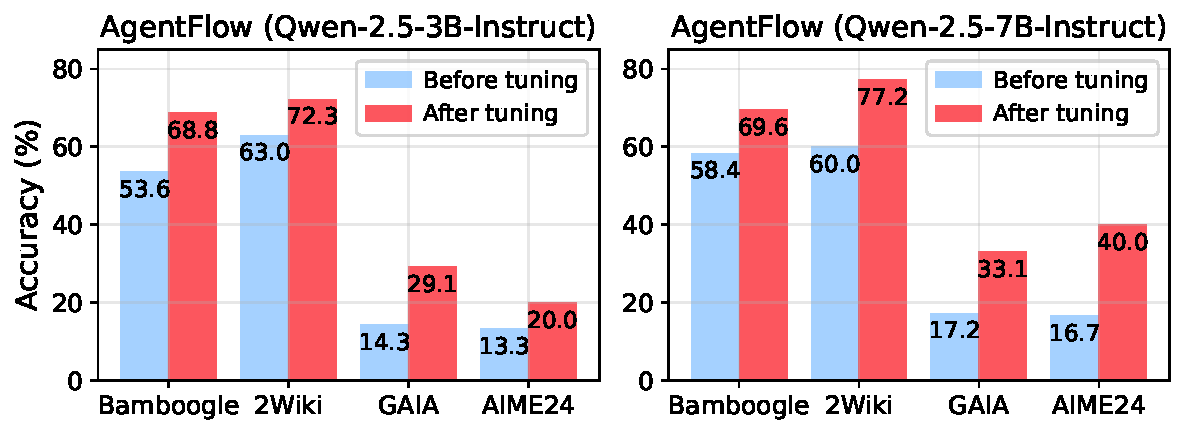
\includegraphics[width=0.95\linewidth]{figs/scaling_model_size.pdf}
        \vspace{-2mm}
        \caption{Flow-GRPO fine-tuning offers consistent gains on \model as the backbone model size scales from 3B to 7B.}
        \label{fig:scaling_model_size}
    \end{minipage}
    \hfill %
    \begin{minipage}[b]{0.32\textwidth}
        \centering
        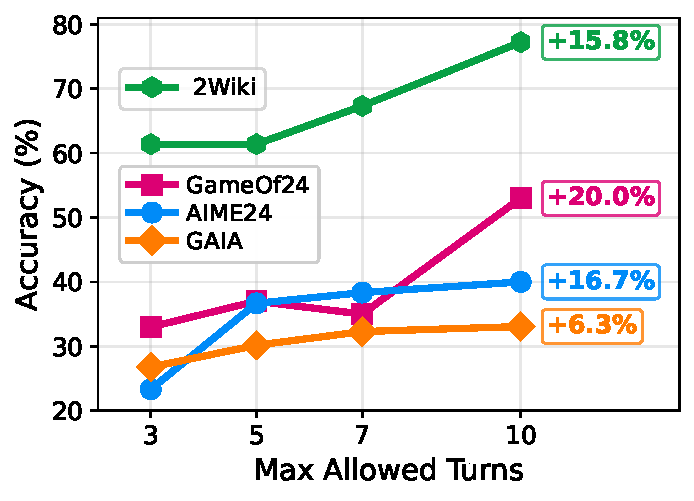
\includegraphics[width=0.95\linewidth]{figs/scaling_turn.pdf}
        \vspace{-2mm}
        \caption{Average accuracy with increased $T_{\text{max}}$.}
        \label{fig:scaling_turn}
    \end{minipage}
    \vspace{-3mm}
\end{figure}

\begin{wraptable}{r}{0.45\textwidth}
    \centering
    \vspace{3pt}
    \footnotesize
    
    \resizebox{\linewidth}{!}{
        \setlength{\tabcolsep}{0.5em}
        \renewcommand{\arraystretch}{0.9}
        \begin{tabular}{lcccc}
            \toprule
            \textbf{Turns ($T_{\text{max}}$)} & \textbf{3} & \textbf{5} & \textbf{7} & \textbf{10} \\
            \midrule
            2Wiki & 2.22 & 3.18 & 3.81 & 4.44 \\
            GameOf24 & 1.63 & 2.12 & 2.36 & 2.67 \\
            AIME24 & 1.63 & 1.63 & 1.86 & 1.90 \\
            GAIA & 2.43 & 3.46 & 4.28 & 5.42 \\
            \bottomrule
        \end{tabular}
    }
    
    \vspace{-2mm} %
    \caption{Average turns with increased $T_{\text{max}}$.}
    \label{tab:scaling_turn} %
    \vspace{-5mm} %
\end{wraptable}

\paragraph{Inference scaling in turn budgets.}
We investigate how the maximum allowed turns ($T_{\text{max}}$) affect reasoning depth and final performance of \model during test-time inference with the Qwen2.5-7B-Instruct backbone. As shown in Figure~\ref{fig:scaling_turn}, increasing $T_{\text{max}}$ from 3 to 10 consistently improves outcomes across all tasks, accompanied by a rise in average turns consumed. On knowledge-intensive benchmarks such as 2Wiki and GAIA, a larger turn budget enables \model for deeper information retrieval. On mathematical benchmarks like GameOf24 and AIME24, it supports decomposed sub-goals, alternative strategies, and refinement of errors. Final performance peaks at $T_{\text{max}}=10$ for all tasks, confirming that a longer reasoning horizon benefits the system without causing degenerate loops. This validates that \model adapts its turn allocation to problem complexity to achieve better solutions through iterative refinement.


\subsection{In-depth Analysis of Optimized Planning}
\label{subsec:optimized_planning}

\begin{wrapfigure}{r}{0.6\textwidth} 
    \centering
    \vspace{-10pt} %
    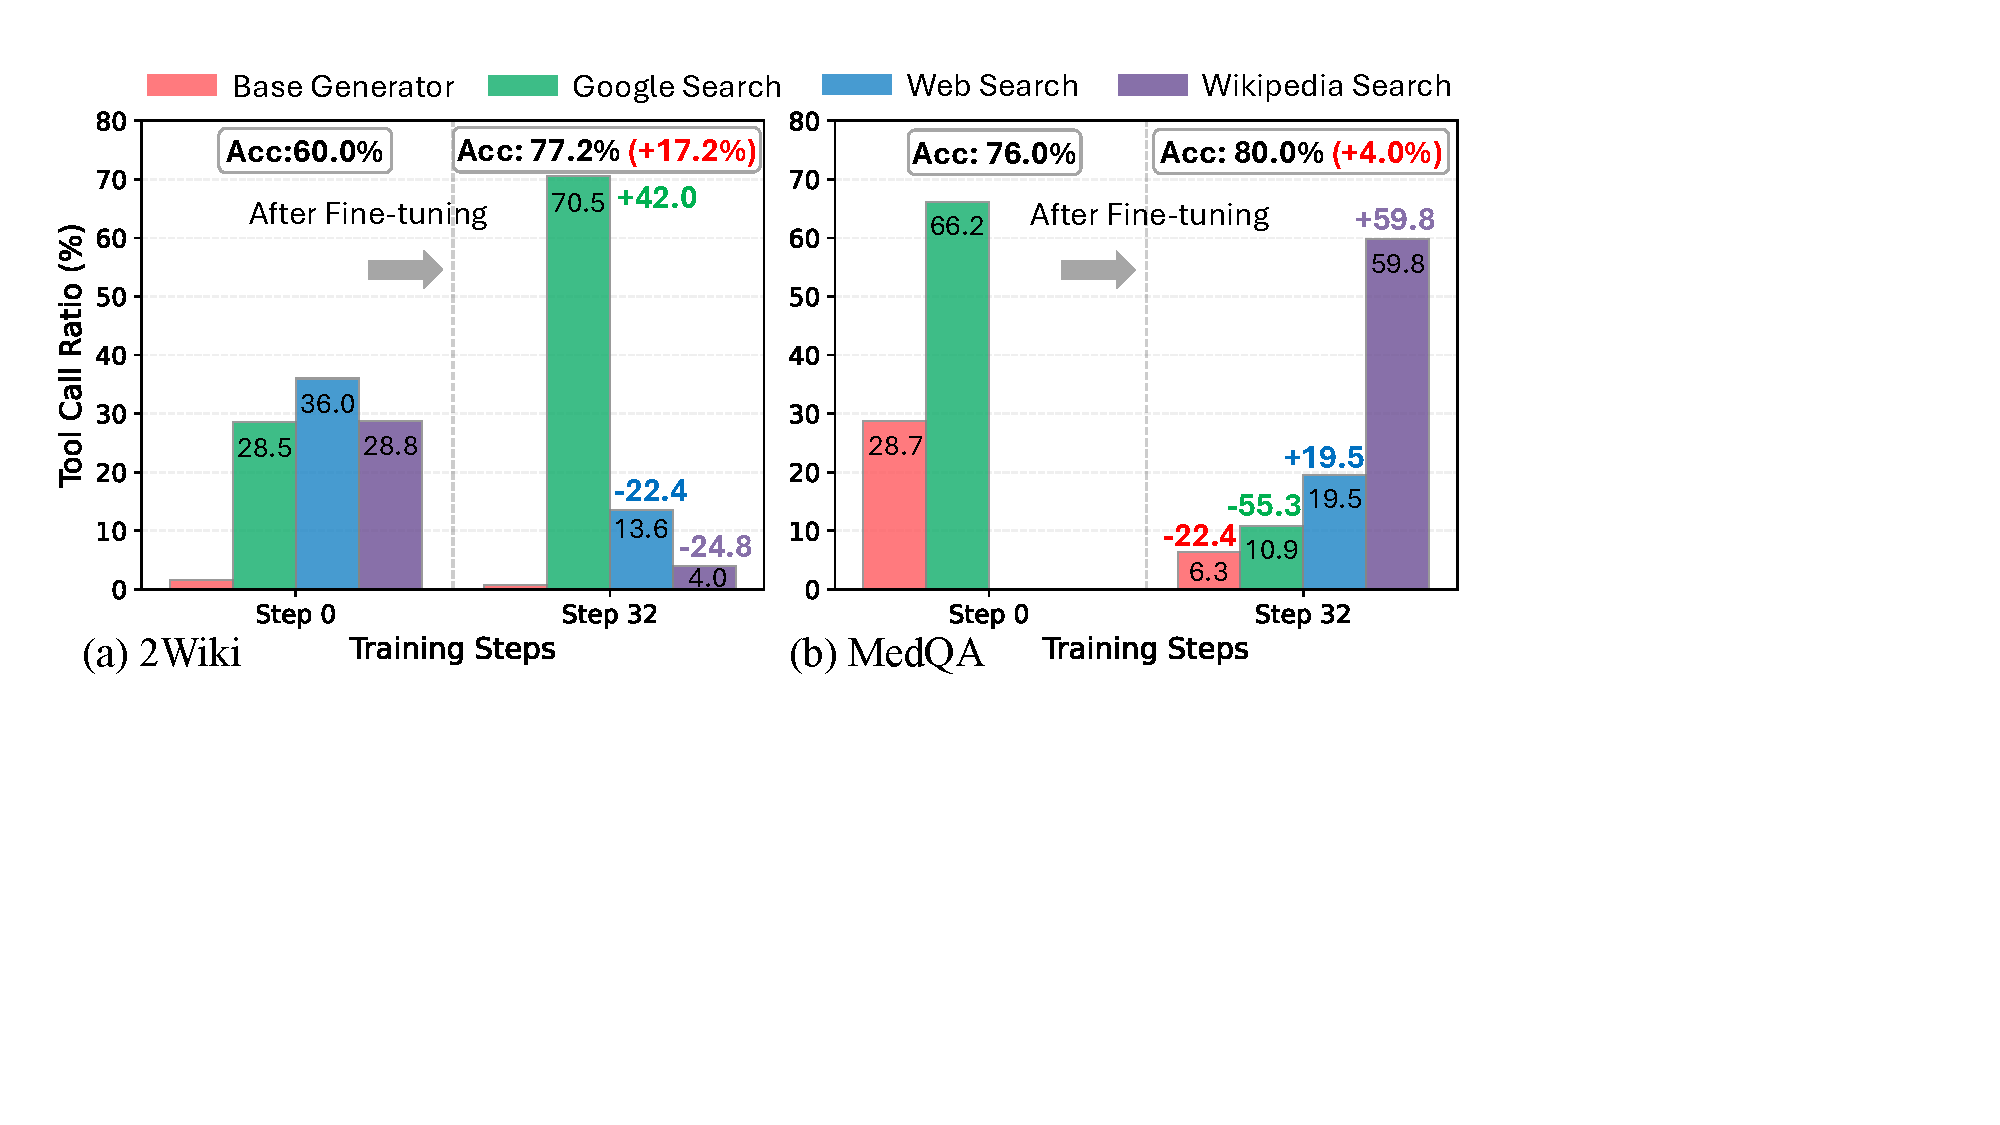
\includegraphics[width=\linewidth]{figs/tool_usage.pdf}
    \vspace{-10pt}
    \caption{Tool call ratio change by Flow-GRPO fine-tuning.}
    \label{fig:tool_usage}
    \vspace{-12pt} %
\end{wrapfigure}

\paragraph{Flow-GRPO optimizes tool usage.} 
We compare tool usage distributions before and after in-the-flow RL training. Figure~\ref{fig:tool_usage} shows results on two knowledge-intensive tasks, 2Wiki and MedQA, which exhibit distinct optimization patterns alongside improved task accuracy. For 2Wiki, which requires broad factual knowledge, Flow-GRPO optimizes the planner to increase Google Search usage by 42.0\%. In contrast, for the specialized MedQA benchmark, which requires deep, domain-specific information retrieval, fine-tuning shifts the planner away from general tools, reducing Google Search calls (66.2$\rightarrow$10.9\%) in favor of in-document Web Search (0$\rightarrow$19.5\%) and specialized  Wikipedia Search (0$\rightarrow$59.8\%). This demonstrates that the planner learns to select task-appropriate tools. 

\paragraph{Flow-GRPO incentivizes autonomous discovery of new solutions.} 
We further examine qualitative examples in Figure~\ref{fig:fig_case_study} and additional cases in \S\ref{app:case_studies}. These cases show that \model, trained with Flow-GRPO, develops enhanced capabilities for task planning and tool use. The planner exhibits adaptive efficiency, stronger self-correction, and spontaneous new integration of tools throughout step-by-step problem-solving, autonomously discovering effective solution pathways.


\vspace{-1mm}
\subsection{Training Efficiency Analysis}
\label{subsec:traing_efficency}


\paragraph{Optimized planning with increased rewards and condensed responses.}
We analyze the training dynamics of the \model planner by tracking its average reward and response length on the train set (Figure~\ref{fig:training_reward}a). Training rewards steadily increase, indicating effective policy improvement via Flow-GRPO. Meanwhile, response length, after an initial exploratory rise, progressively shortens and stabilizes. This shows the planner learns to balance conciseness and informativeness, avoiding unnecessarily long outputs.

\begin{wrapfigure}{r}{0.60\textwidth}
    \centering
    \begin{subfigure}[t]{0.49\linewidth}
    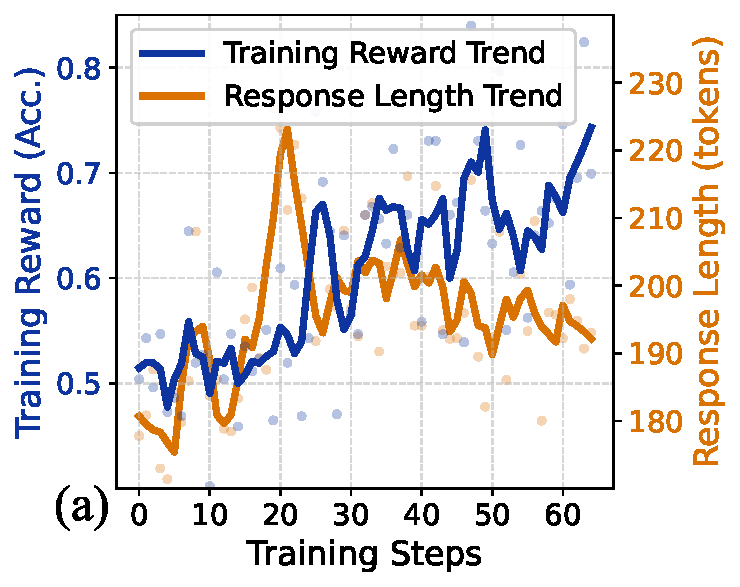
\includegraphics[height=0.15\textheight,keepaspectratio]{figs/train_reward.pdf}
    \end{subfigure}
    \hfill
    \begin{subfigure}[t]{0.45\linewidth}
        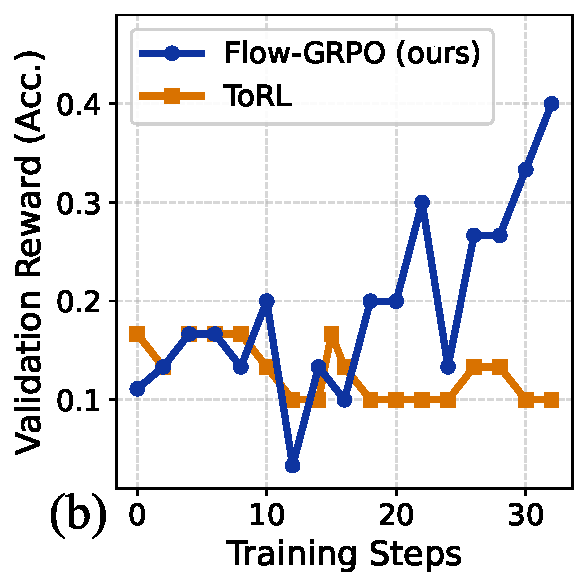
\includegraphics[height=0.15\textheight,keepaspectratio]{figs/val_reward_comp.pdf}
    \end{subfigure}
    \vspace{-2mm}
    \caption{Training dynamics and efficiency of Flow-GRPO.}
    \label{fig:training_reward}
    \vspace{-2mm}
\end{wrapfigure}

\paragraph{Flow-GRPO efficiency over tool-integrated reasoning RL.}
We compare \model (trained with Flow-GRPO) against a monolithic tool-integrated reasoning baseline (ToRL) on AIME24. As shown in Figure~\ref{fig:training_reward}b, \model achieves sustained performance gains, with validation accuracy growing steadily. In contrast, ToRL's performance quickly stagnates and trends downwards, highlighting the superior efficiency of our agentic training approach, which uses decomposition and stable credit assignment to avoid the instability.

\vspace{-1mm}




\vspace{-2mm}
\section{Related Work}
\label{sec:related_work}
\vspace{-1mm}

Reinforcement learning (RL) from outcome-based rewards has become a dominant paradigm for training LLMs to use external tools. Much of this work trains a single, monolithic policy to interleave reasoning with tool calls. This strategy has proven effective in specialized, single-tool settings~\citep{mai2025agent, xue2025simpletir, feng2025retool, li2025torl} and web search for knowledge-intensive questions~\citep{chen2025research, jin2025search, song2025r1, li2025search, sun2025zerosearch}. Recent efforts have extended this monolithic framework to multi-tool environments by focusing on data synthesis \citep{dong2025tool}, unified training infrastructure \citep{jiang2025verltool}, and principled reward design \citep{qian2025toolrl, zhang2025nemotron}. However, these approach scales poorly as task complexity and planning horizons grow. The central challenge is long-horizon credit assignment; attributing a final outcome to specific intermediate tool calls remains difficult, even with fine-grained, turn-level rewards~\citep{zeng2025reinforcing, wang2025stepsearch}. This difficulty leads to training instability and brittle inference-time generalization, manifesting as strategic deficiencies like tool overuse or ``cognitive offloading''~\citep{Wang2025ActingLI, qian2025smart}, suboptimal personalization~\citep{cheng2025toolspectrum}, and poor alignment with user preferences for tool invocation~\citep{huang2025ttpa}.

\paragraph{Agentic systems with tool use.}
Agentic systems offer an alternative to monolithic models by decomposing tasks across specialized modules. Many such systems are training-free, orchestrating pre-trained LLMs with handcrafted logic and prompting, as seen in frameworks like AutoGen~\citep{wu2024autogen}, MetaGPT~\citep{hong2024metagpt}, and OctoTools~\citep{lu2025octotools}. This static approach, however, limits their ability to learn and adapt collaborative strategies from experience. Recognizing this, recent work explores training these systems to improve coordination~\citep{deng2025pe, liao2025marft}. However, most training paradigms are \emph{offline}, relying on supervised fine-tuning or preference optimization on static datasets~\citep{motwani2024malt, park2025maporl}. These methods are decoupled from the live, multi-turn dynamics of the system, preventing modules from learning to adapt to evolving tool outputs or recover from early mistakes. Training directly \emph{in the flow} with on-policy RL is difficult due to sparse rewards and long-horizon credit assignment, where feedback is delayed across long reasoning chains and shifting state distributions~\citep{wang2025ragen}. Consequently, these systems often suffer from brittle adaptation and require complex reward shaping to learn effectively~\citep{wang2025spa}.



\vspace{-2mm}
\section{Conclusion}
\vspace{-1mm}


We presented \model, a trainable, \emph{in-the-flow} agentic system that coordinates four specialized modules via an evolving memory and optimizes its planner directly \emph{inside} the multi-turn loop. To enable stable on-policy learning under long-horizon, sparse-reward settings, we introduced Flow-GRPO, which \emph{converts} multi-turn RL into a sequence of tractable \emph{single-turn} policy updates by \emph{broadcasting} a single, verifiable trajectory-level outcome to every turn and stabilizing credit assignment with group-normalized advantages. Comprehensive experiments show that \model achieves strong cross-domain performance, surpassing specialized baselines and even larger proprietary models. In-depth analyses confirm improved planning and tool-calling reliability, along with positive scaling trends in model size and allowed turn budgets.

\section*{Acknowledgment}
We would like to thank Yihe Deng, Xuehang Guo, and Kunlun Zhu for their valuable input during the early stages of this work. We are also grateful to Lambda for providing GPU resources. This work was partially supported by the Hoffman-Yee Research Grants program at Stanford HAI, the AI for Math Fund by Renaissance Philanthropy, ONR MURI N00014-24-1-2748, and the AI Research Hub Project through KAIST. This work was also supported by IITP (No.~RS-2024-00457882, National AI Research Lab Project).


\bibliography{iclr2026_conference}
\bibliographystyle{iclr2026_conference}

\clearpage
\appendix

\renewcommand*\footnoterule{} %

\newcommand\blfootnote[1]{%
  \begingroup
  \renewcommand\thefootnote{}\footnote{#1}%
  \addtocounter{footnote}{-1}%
  \endgroup
}

\section*{Table of Contents}
\setcounter{tocdepth}{2}
\renewcommand{\contentsname}{Appendix Contents}
\startcontents[appendix]  %
\printcontents[appendix]{}{1}{}





\clearpage
\section{Training Algorithm of \model}
\label{app:details_of_model}


We provide a flowchart of the overall training algorithm of \model (\S\ref{sec:methodology}) in Algorithm~\ref{alg:agentflow}.

\begin{algorithm}
\caption{In-the-Flow Optimization for \model}
\label{alg:agentflow}
\begin{algorithmic}[1]
\REQUIRE Dataset $\mathcal{D}$, Action Planner policy $\pi_\theta$, Tool Executor $\mathcal{E}$, Executive Verifier $\mathcal{V}$, Solution Generator $\mathcal{G}$, Toolset $K$, and Shared Evolving Memory ${M}$


\ENSURE Optimized Action Planner parameters $\theta^\star$

\FOR{each training iteration}

    \FOR{each query–label pair $(q, y^*) \sim \mathcal{D}$}
    
    \STATE \textbf{\textsc{1. In-the-Flow Rollout Generation}}
    \STATE Initialize: $t \leftarrow 1$, $M^t \leftarrow q$

    \REPEAT
        \STATE $a^{t} \sim \pi_\theta(a^t \mid q, K, M^{t})$ \COMMENT{\textit{Plan Action}} \
        \STATE $e^{t} \sim \mathcal{E}(e^t \mid a^{t}, K)$ \ \COMMENT{\textit{Execute Action}}
        \STATE $v^{t} \sim \mathcal{V}(v^{t} \mid q, e^{t}, M^{t})$ \COMMENT{\textit{Verify Result}}
        \STATE $M^{t+1} = f_{\text{mem}}\!(M^t, a^t, e^t, v^t)$ \COMMENT{\textit{Update Memory}} 
        \STATE $t \leftarrow t + 1$
    \UNTIL{termination condition met}
    
    \STATE $o \sim \mathcal{G}(o \mid q, M^T)$ \COMMENT{\textit{Generate Final Solution}}

    \STATE \textbf{\textsc{2. Reward Computation}}
    
    \STATE $R(a^t) = \bar{R}(o, q, y^*), \quad \forall t = 1,\dots,T$


\STATE \textbf{\textsc{3. Policy Update}}
\STATE Update the Action Planner policy $\pi_\theta$ by maximizing the Flow-GRPO objective (Eq. \ref{eq:Flow-GRPO_objective})
    \ENDFOR
\ENDFOR

\RETURN optimized parameters $\theta^\star$
\end{algorithmic}
\end{algorithm}

\clearpage
\section{Theoretical Analysis of Flow-GRPO}
\label{app:mathematical_analysis}
\subsection{Preliminaries and Notation}

We adopt the notation from the paper to formalize our analysis.

\begin{definition}[Core Components] Here we list core definition of variables. 
\\
\\
{\small
\begin{tabularx}{\textwidth}{@{} l X @{}}
    \multicolumn{2}{@{}l}{\textbf{Symbol and Description}} \\
    \hline \\
    $\pi_{\theta}$ & The trainable planner policy, parameterized by $\theta$. \\
    $\pi_{\theta_{\text{old}}}$ & The behavior policy used to sample trajectories. \\
    $s^t$ & The state at turn $t$, defined as $s^t = (q, K, M_t)$. \\
    $a^t$ & The action (a sequence of tokens) generated at state $s^t$, where $a^t \sim \pi_\theta(\cdot \mid s^t)$. \\
    $\tau$ & A trajectory of states and actions over $T$ time steps, defined as $\tau = \{(s^t, a^t)\}_{t=1}^T$. \\
    $R(\tau)$ & The outcome-based reward for trajectory $\tau$, where $R(\tau) \in \{0,1\}$. \\
    $A_{\tau}$ & The group-normalized advantage for trajectory $\tau$. A crucial property is that the advantage is constant for all timesteps within a trajectory defined in Eq. \ref{eq:advantage_norm}: $a^t = A_{\tau}, \quad \forall (s^t, a^t) \in \tau$.  \\
    $\rho_{i,j}^t$ & The token-level importance sampling ratio, defined as:
    $$ \rho_{i,j}^t
    = \frac{\pi_\theta\!\big(a_{i,j}^t \,\big|\, s_i^t, a_{i,1:j-1}^t\big)}
    {\pi_{\theta_\text{old}}\!\big(a_{i,j}^t \,\big|\, s_i^t, a_{i,1:j-1}^t\big)}. $$ \\
    $L_{\text{clip}}(\rho, A)$ & The PPO clipped objective term, defined as $L_{\text{clip}}(\rho, A) = \min(\rho A, \text{clip}(\rho, 1-\epsilon, 1+\epsilon) A)$. \\
    \hline
    \\
\end{tabularx}
}
\end{definition}
\begin{definition}[Objective Functions]
The \emph{global policy objective} is the expected trajectory-level reward:
\begin{equation}
    \mathcal{J}(\theta) := \E_{\tau \sim \pi_{\theta}}[R(\tau)].
\end{equation}

The \emph{single-turn optimization objective} for a given state $s^t$ is defined as:
\begin{equation}
    \mathcal{J}_{\text{local}}(\theta; s^t) := \E_{a^t \sim \pi_{\theta_{\text{old}}}(\cdot \mid s^t)} \left[ \frac{1}{|a^t|} \sum_{j=1}^{|a^t|} L_{\text{clip}}(\rho_{i, j}^t, A_i^t) \right].
\end{equation}

The full \emph{}{Flow-GRPO objective function} in the multi-turn setting is given by:
\begin{equation}
    \mathcal{J}_{\text{Flow-GRPO}}(\theta) := \E_{\substack{(q,y^*) \sim \mathcal{D} \\ \{\tau_i\}_{i=1}^G \sim \pi_{\theta_{\text{old}}}}} \left[ \frac{1}{G} \sum_{i=1}^G \frac{1}{T_i} \sum_{t=1}^{T_i} \frac{1}{|a^t_i|} \sum_{j=1}^{|a^t_i|} L_{\text{clip}}(\rho_{i,j}^t, A_i^t) \right] - \beta \mathbb{D}_{\mathrm{KL}}(\pi_\theta \| \pi_{\text{ref}}).
\end{equation}
\end{definition}

\subsection{Equivalence Proof for Optimization Objectives}


\begin{theorem}    
In Flow-GRPO, maximizing the global multi-turn objective is mathematically equivalent to maximizing the expected token-level local objective at each time step under the on-policy induced state distribution, given standard sampling assumptions (trajectories sampled i.i.d. from the policy with fixed finite turn $T$).
\end{theorem}


\begin{proof}
\label{app:proof_clip_term_equalization}
Let's denote the clipping part of the Flow-GRPO objective as $\mathcal{J}_{\text{clip}}(\theta)$.

First, by the linearity of expectation, we can simplify the expectation over a group of $G$ trajectories. Since the trajectories $\{\tau_i\}$ are sampled independently and identically (i.i.d.) from the behavior policy $\pi_{\theta_{\text{old}}}$, the expectation of their average is equal to the expectation over a single trajectory.
\begin{align}
    \mathcal{J}_{\text{clip}}(\theta) &= \E_{(q,y^*) \sim \mathcal{D}} \left[ \E_{\{\tau_i\}_{i=1}^G \sim \pi_{\theta_{\text{old}}}} \left[ \frac{1}{G} \sum_{i=1}^G \frac{1}{T_i} \sum_{t=1}^{T_i} \left( \frac{1}{|a^t_i|} \sum_{j=1}^{|a^t_i|} L_{\text{clip}}(\rho_{i,j}^t, A_i^t) \right) \right] \right] \\
    &= \E_{(q,y^*) \sim \mathcal{D}} \left[ \E_{\tau \sim \pi_{\theta_{\text{old}}}(\cdot|q)} \left[ \frac{1}{T} \sum_{t=1}^{T} \left( \frac{1}{|a^t|} \sum_{j=1}^{|a^t|} L_{\text{clip}}(\rho^t_j, A_\tau) \right) \right] \right].
\end{align}
Here, $\tau = \{(s^t, a^t)\}_{t=1}^T$ represents a single, arbitrarily sampled trajectory with advantage $A_\tau$.

Next, we can re-interpret the expectation over trajectories as an expectation over the state-visitation distribution induced by the policy $\pi_{\theta_{\text{old}}}$. Let $d^{\pi_{\theta_{\text{old}}}}$ be the on-policy distribution of states visited, where each state $s^t$ in a trajectory of length $T$ is weighted by $1/T$. The expectation can be rewritten as:
\begin{align}
    \mathcal{J}_{\text{clip}}(\theta) &= \E_{(q,y^*) \sim \mathcal{D}} \left[ \E_{s^t \sim d^{\pi_{\theta_{\text{old}}}}} \left[ \E_{a^t \sim \pi_{\theta_{\text{old}}}(\cdot|s^t)} \left[ \frac{1}{|a^t|} \sum_{j=1}^{|a^t|} L_{\text{clip}}(\rho^t_j, A^t) \right] \right] \right].
\end{align}
Note that $A^t$ is the advantage corresponding to the trajectory from which $s^t$ was sampled.

We now recognize that the inner expectation is precisely the definition of the local, per-state objective, $\mathcal{J}_{\text{local}}(\theta; s^t)$.
\begin{align}
    \mathcal{J}_{\text{clip}}(\theta) &= \E_{(q,y^*) \sim \mathcal{D}, \ s^t \sim d^{\pi_{\theta_{\text{old}}}}} \left[ \mathcal{J}_{\text{local}}(\theta; s^t) \right].
\end{align}
Adding the KL-divergence term back, we arrive at the final equivalence:
\begin{equation}
    \mathcal{J}_{\text{Flow-GRPO}}(\theta) = \E_{(q,y^*) \sim \mathcal{D}, \ s^t \sim d^{\pi_{\theta_{\text{old}}}}} \left[ \mathcal{J}_{\text{local}}(\theta; s^t) \right] - \beta \mathbb{D}_{KL}(\pi_\theta \| \pi_{\text{ref}}).
\end{equation}
This proves that maximizing the global multi-turn Flow-GRPO objective is equivalent to maximizing the expected token-level local objective at each time step under the on-policy induced state distribution.
\end{proof}


\subsection{Convergence Analysis}
Having established the structural validity of the objective, we now analyze its convergence properties. 
The analysis builds on the monotonic improvement guarantee provided by trust-region methods~\citep{schulman2015trust}.

\begin{lemma}[Policy Performance Difference]
For two policies $\pi_{\theta}$ and $\pi_{\theta_{\rm old}}$, the difference in expected return can be expressed as:
\begin{equation}
\mathcal{J}(\theta) - \mathcal{J}(\theta_{\rm old}) 
= \E_{\tau \sim \pi_{\theta}} \left[ \sum_{t=1}^{T} \, A_{\theta_{\rm old}}(s^t, a^t) \right],
\end{equation}
where $A_{\theta_{\rm old}}$ is the advantage function under the old policy.
\end{lemma}

This lemma enables the construction of a lower bound on policy improvement.

\begin{theorem}[Monotonic Improvement Guarantee]
Define the surrogate objective
\begin{equation}
\mathcal{L}_{\theta_{\rm old}}(\theta) 
= \E_{\tau \sim \pi_{\theta_{\rm old}}} \left[ \sum_{t=1}^{T} \, 
\frac{\pi_{\theta}(a^t|s^t)}{\pi_{\theta_{\rm old}}(a^t|s^t)} \, A_{\theta_{\rm old}}(s^t, a^t) \right].
\end{equation}
Then the performance improvement satisfies the lower bound
\begin{equation}
\mathcal{J}(\theta) - \mathcal{J}(\theta_{\rm old}) 
\;\;\ge\;\; \mathcal{L}_{\theta_{\rm old}}(\theta) 
- C \cdot \bar{\mathbb{D}}_{\mathrm{KL}}\!\left(\pi_{\theta_{\rm old}}, \pi_{\theta}\right),
\end{equation}
where $C > 0$ is a constant depending on the horizon and reward scale, and 
$\bar{\mathbb{D}}_{\mathrm{KL}}$ denotes the average KL-divergence between the two policies.
\end{theorem}

By optimizing the right-hand side of the above inequality, we are guaranteed to improve the performance of $\pi_\theta$. Therefore, for policies $\pi_\theta^t$ and $\pi_\theta^{t+1}$ obtained from iterations $t$ and $t+1$, we have:
\begin{equation}
\mathcal{J}(\theta^{t+1}) \geq \mathcal{J}(\theta^t).
\end{equation}













\textbf{Conclusion.}
This analysis establishes that Flow-GRPO optimizes a valid surrogate objective and guarantees monotonic policy improvement, thereby converging reliably to a locally optimal policy.



\clearpage
\section{Experimental Details}
\label{app:exp_details}

\subsection{Training Details}
\label{app:training_details}


We provide further details on the training setup for \model. Our Flow-GRPO implementation uses a learning rate of $1 \times 10^{-6}$. The Action Planner generates actions with a sampling temperature of $0.5$ to balance exploration and exploitation. To prevent policy collapse and stabilize training, we incorporate a KL-divergence penalty against a reference policy with a coefficient $\beta = 0.001$. The maximum output length for the planner is set to 2048 tokens to ensure complete exploration during rollouts.

To accelerate the training speed, we limit the maximum number of turns per rollout to $3$. The final-outcome reward signal (Eq.~\ref{eq:reward_func}) is provided by an LLM-as-judge, for which we use \textit{GPT-4o}. All tool calls are executed synchronously with a 500-second timeout to handle external service latency robustly. The LLM engines within the tools are set to a temperature of 0.0 to ensure deterministic and stable outputs. The full training process was conducted on 8 NVIDIA A100 GPUs. Further details on agent prompts and the memory update mechanism are provided in \S\ref{app:modules_and_memory}.


\subsection{Evaluation Details}
\label{app:eval_details}
Here, we outline the specifics of our evaluation protocol. For evaluation, we increase the maximum number of turns per rollout to $T=10$ to allow for more extensive and deeper reasoning. The planner's sampling temperature is set to 0.7 to encourage diverse solution paths. Unless otherwise specified, all tool LLM engines are initialized with Qwen2.5-7B-Instruct.

For fair and consistent evaluation, we adopt the previous work's methodology while standardizing tools: we replace search tools in search-enhanced models with our Google Search tool and code tools in code-enhanced models with our Python Coder tool. We use GPT-4o as an LLM-based judge to determine the correctness of final answers. This approach provides a robust measure of semantic and numerical equivalence, which is critical for complex reasoning tasks. The specific judging prompt is detailed in \S\ref{app:llm_based_judging}, and additional information on evaluation datasets can be found in \S\ref{app:datasets}. To mitigate randomness, we report the average accuracy with standard deviation across three trials for all experiments.


\subsection{Compared Baselines}
\label{app:baseline}
\textbf{Proprietary LLMs:}
\begin{itemize}[leftmargin=1em]

\item \textbf{Qwen2.5 Series}~\citep{yang2024qwen2.5}, created by Alibaba, comes in multiple configurations. These models undergo training on multilingual corpora covering 29 different languages, demonstrating superior performance in cross-lingual applications. Furthermore, Qwen2.5 showcases robust proficiency in programming and mathematical domains. 


\item \textbf{Llama-3 Series}~\citep{dubey2024llama}, created by Meta AI, encompasses various iterations. Each model configuration within the Llama family provides dual versions: foundational and instruction-following variants. Training incorporates diverse dataset combinations spanning multiple domains and linguistic varieties. The Llama model family demonstrates excellent results in logical reasoning, software development, and cross-lingual comprehension evaluations. Through progressive enhancements in fine-tuning methodologies and expanded sequence lengths, these models become more applicable to practical deployment scenarios.

\item \textbf{GPT-4o Series}~\citep{hurst2024gpt}, produced by OpenAI, includes several model variants such as GPT-4o and GPT-4o-mini, with training leveraging extensive multimodal datasets encompassing text, vision, and audio modalities. The series achieves outstanding performance in complex reasoning tasks, creative generation, and multimodal understanding benchmarks with continuous refinements in alignment techniques and enhanced processing capabilities.
\end{itemize}

\textbf{Reasoning LLMs:}
\begin{itemize}[leftmargin=1em]
\item \textbf{SFT}~\citep{zeng2025simplerl} serves as our basic baseline following Search-R1 \citep{jin2025search}. We fine-tune models using supervised fine-tuning on GPT-4o-generated reasoning chains. 


\item \textbf{SimpleRL-Zoo}~\citep{zeng2025simplerl} investigates zero reinforcement learning training across 10 diverse base models spanning different families and sizes using GRPO algorithm with simple rule-based rewards, achieving substantial improvements in reasoning accuracy. 

\item \textbf{Open-Reasoner-Zero}~\citep{hu2025open} presents the first open-source implementation of large-scale reasoning-oriented RL training using PPO with GAE and straightforward rule-based rewards, without KL regularization. The framework demonstrates that minimalist design can successfully scale both response length and benchmark performance. 


\item \textbf{General-Reasoner}~\citep{ma2025general} extends LLM reasoning capabilities beyond mathematics to diverse domains using RLVR through a 230K verifiable reasoning questions dataset spanning physics, chemistry, and finance.

\item \textbf{LUFFY}~\citep{yan2025learning} addresses limitations in on-policy RLVR by introducing an off-policy framework that augments training with external reasoning demonstrations using Mixed Policy GRPO and regularized importance sampling.


\end{itemize}

\textbf{Search-Integrated Reasoning LLMs:}
\begin{itemize}[leftmargin=1em]
\item \textbf{Iter-RetGen}~\citep{shao2023enhancing} addresses limitations in retrieval-augmented language models by introducing iterative retrieval-generation synergy, where a model's previous response serves as context for retrieving more relevant knowledge in subsequent iterations. 


\item \textbf{Search-R1}~\citep{jin2025search} represents a reinforcement learning approach that develops a model from the ground up to invoke search functionality throughout the reasoning process.


\item \textbf{ZeroSearch}~\citep{sun2025zerosearch} addresses high API costs in RL-based search training by using an LLM to simulate search engines, employing lightweight supervised fine-tuning to transform an LLM into a retrieval module that generates both useful and noisy documents. The framework combines this with a curriculum-based rollout strategy that progressively degrades document quality, achieving better performance than real search engine-based methods while incurring zero API costs.


\item \textbf{ReSearch}~\citep{chen2025research} proposes a reinforcement learning framework that trains LLMs to integrate search operations as components of the reasoning chain without supervised data on reasoning steps, treating search decisions as guided by text-based thinking. 

\item \textbf{StepSearch}~\citep{wang2025stepsearch} addresses the sparse reward problem in multi-hop reasoning by training search LLMs using step-wise proximal policy optimization with intermediate rewards and token-level process supervision based on information gain and redundancy penalties. 

\item \textbf{VerlTool}~\citep{jiang2025verltool} addresses fragmentation and synchronization bottlenecks in Agentic Reinforcement Learning with Tool use by introducing a unified modular framework that extends beyond single-turn RLVR paradigms, providing upstream VeRL alignment and unified tool management with asynchronous rollout execution achieving near 2× speedup. 
\end{itemize}

\textbf{Code-Integrated Reasoning LLMs:}
\begin{itemize}[leftmargin=1em]
\item \textbf{TIR}~\citep{yang2024qwen2} is a basic baseline that demonstrates the model's ability to generate code for tool utilization. In our implementation, we directly prompt the model to write code that calls the programming interpreter and processes the returned results to generate the final answer.

\item \textbf{ToRL}~\citep{li2025torl} is a code-enhanced architecture developed via reinforcement learning that empowers models to independently activate code execution environments for mathematical reasoning tasks.
\end{itemize}

\textbf{Training-free Agentic System}

\begin{itemize}[leftmargin=1em]
\item \textbf{AutoGen}~\citep{wu2024autogen} introduces an agentic conversation framework that enables developers to build LLM applications through conversable agents that can operate using combinations of LLMs, human inputs, and tools.
\end{itemize}



\subsection{Evaluation Datasets}
\label{app:datasets}
We provide a detailed introduction to the \textit{search-intensive} and \textit{agentic} benchmarks in our experiments as follows:

\begin{itemize}[leftmargin=1em]
    \item \textbf{Bamboogle}~\citep{press2023measuring} presents a demanding multi-step reasoning dataset containing manually constructed questions requiring up to four inferential steps. The dataset evaluates models' capacity for intricate compositional reasoning across interconnected facts.
    \item \textbf{2Wiki (2WikiMultihopQA)}~\citep{ho2020constructing} constitutes a comprehensive multi-step QA corpus combining structured Wikidata knowledge with unstructured Wikipedia text. The dataset encompasses varied question formats and annotated reasoning chains to facilitate interpretable sequential inference. We randomly sample 100 examples as a test set for efficiency.
    \item \textbf{HotpotQA}~\citep{yang2018hotpotqa} represents a widely-adopted question answering corpus featuring multi-step queries constructed from Wikipedia entries. We randomly sample 100 examples as a test set for efficiency.
    \item \textbf{Musique}~\citep{trivedi2022musique} comprises a multi-step reasoning corpus requiring sequential inference where each reasoning stage depends on information derived from preceding steps. We conduct evaluations using the development partition of this particularly challenging dataset. We randomly sample 100 examples as a test set for efficiency.
    \item \textbf{GAIA}~\citep{mialon2023gaia} constitutes a benchmark engineered to assess general AI systems and agents, demanding capabilities including sequential reasoning, web navigation, and comprehensive tool utilization skills. We utilize the text-exclusive portion of this dataset, designed to challenge base language models in our experimental setup.
\end{itemize}



Furthermore, we also conduct a series of experiments on \textit{math} and \textit{scientific reasoning} benchmarks:
\begin{itemize}[leftmargin=1em]
\item \textbf{AIME24} \citep{aops_aime} A collection of 30 demanding mathematical problems sourced from the 2024 American Invitational Mathematics Examination (AIME), encompassing algebra, geometry, number theory, and combinatorics. Each JSONL-formatted record contains the problem identifier, question text, comprehensive solution methodology, and the final numerical result. Created to assess large language models' sophisticated mathematical reasoning abilities, the dataset presents substantial difficulty, systematic multi-phase solutions, and distinctive answers—establishing it as a robust benchmark for evaluating advanced analytical capabilities.
\item \textbf{AMC23} \citep{AMC23} contains mathematical problems derived from the 2023 American Mathematics Competition, emphasizing areas such as functional equations and complex analysis.
\item \textbf{GameOf24} \citep{24game} derives from the traditional numerical puzzle known as 24 (alternatively called the 24 numbers game). The challenge requires utilizing four given numbers with fundamental arithmetic operations (addition, subtraction, multiplication, division) to create an expression yielding 24. For instance, with numbers 4, 9, 10, and 13, a correct solution would be ``(10 - 4) × (13 - 9) = 24''. Successfully solving requires computational proficiency along with iterative attempts to validate potential solutions. Each challenge is formatted as open-ended inquiries. 
\item \textbf{GPQA} or Graduate Level Google-Proof Q\&A Benchmark \citep{rein2024gpqa} comprises a collection of demanding text-based multiple choice problems authored by subject specialists in biology, physics, and chemistry, intentionally crafted to be ``exceptionally challenging''. We randomly sample 100 examples as a test set for efficiency.
\item \textbf{MedQA}~\citep{jin2021disease} features text-based multiple choice problems assembled from professional medical licensing examinations. Problems encompass comprehensive medical knowledge and clinical reasoning skills.

\end{itemize}


\clearpage
\section{More Discussion about Experiment Results}
\subsection{Main Result Analysis}
\label{app:main_result_analysis}
Our main results are presented in Tables \ref{tab:main_table_search_agentic} and \ref{tab:main_table_math_science}. Overall, \model consistently outperforms all baseline models across diverse domains, including search-intensive tasks, agentic tasks, and mathematical and scientific reasoning tasks. These comprehensive results yield several key insights:


\textbf{Monolithic LLMs are insufficient for complex reasoning.} While scaling up model size (from 7B model to GPT-4o) improves average performance, their monolithic nature presents limitations when facing complex tasks that require multi-turn reasoning and sub-goal decomposition. In contrast, our proposed \model consistently outperforms these larger models. Specifically, it achieves an average improvement of 8.2\% over GPT-4o on search-intensive tasks (57.3\% vs.\ 49.1\% in Table~\ref{tab:main_table_search_agentic}), and a remarkable 15.8\% gain over GPT-4o on agentic tasks (33.1\% vs.\ 17.3\% in Table~\ref{tab:main_table_search_agentic}). For mathematical reasoning benchmarks, \model obtains a substantial improvement of 16.4\% over GPT-4o (51.5\% vs.\ 35.1\% in Table~\ref{tab:main_table_math_science}). Furthermore, it surpasses the strong Llama-3.3-70B by 12.5\% on scientific reasoning tasks (63.5\% vs.\ 51.0\% in Table~\ref{tab:main_table_math_science}). These results demonstrate that the carefully designed agentic system of \model, despite being built on a 7B-parameter backbone, can deliver superior and more efficient performance compared to substantially larger monolithic LLMs.  



\textbf{Specialized reasoning models exhibit strong in-domain focus but limited generalizability.}  
While domain-specific fine-tuning and tailored tool integration provide clear benefits over base LLMs, they fail to deliver robust cross-domain performance due to fundamental scaling limitations. Our evaluation across three reasoning domains substantiates these limitations. On search-intensive tasks, specialized models such as Search-R1 (33.3\%) and VerlTool (39.0\%) perform well within their narrow scope yet fall substantially short of \model (57.3\%) as shown in Table~\ref{tab:main_table_search_agentic}. Similarly, in mathematical reasoning, methods like SimpleRL-reason (36.6\%) and ToRL (37.0\%) trail significantly behind \model (51.5\%) in Table~\ref{tab:main_table_math_science}. Even in scientific reasoning, where models such as Luffy (55.5\%) offer competitive results, they are consistently surpassed by \model (63.5\%) in Table~\ref{tab:main_table_math_science}. These findings demonstrate that while specialized reasoning models excel within narrow domains, their reliance on a single monolithic policy introduces poor generalization, making them brittle when confronted with diverse, cross-domain challenges.

\textbf{\model demonstrates superior, versatile reasoning through its adaptive agentic system.}
\model establishes a new state-of-the-art agentic system by achieving an average accuracy of 57.3\% on search-intensive tasks, 33.1\% on agentic tasks, 51.5\% on mathematical reasoning, and 63.5\% on scientific reasoning. Our method's advantage stems from combining an agentic system with targeted planning policy refinement via on-policy reinforcement learning in an online fashion. When compared to AutoGen---a general agent framework with the same backbone model---\model demonstrates a massive improvement of 14.9\% on search tasks and 19.9\% on math tasks. This underscores that the core advantage comes from our dedicated trainable agentic system that integrates our novel Flow-GRPO for in-system on-policy optimization, enabling effective agent planning and tool utilization to solve complex, long-horizon problems across diverse domains.



\begin{figure}[!ht]
\centering
\begin{minipage}[b]{0.48\textwidth}
    \centering
    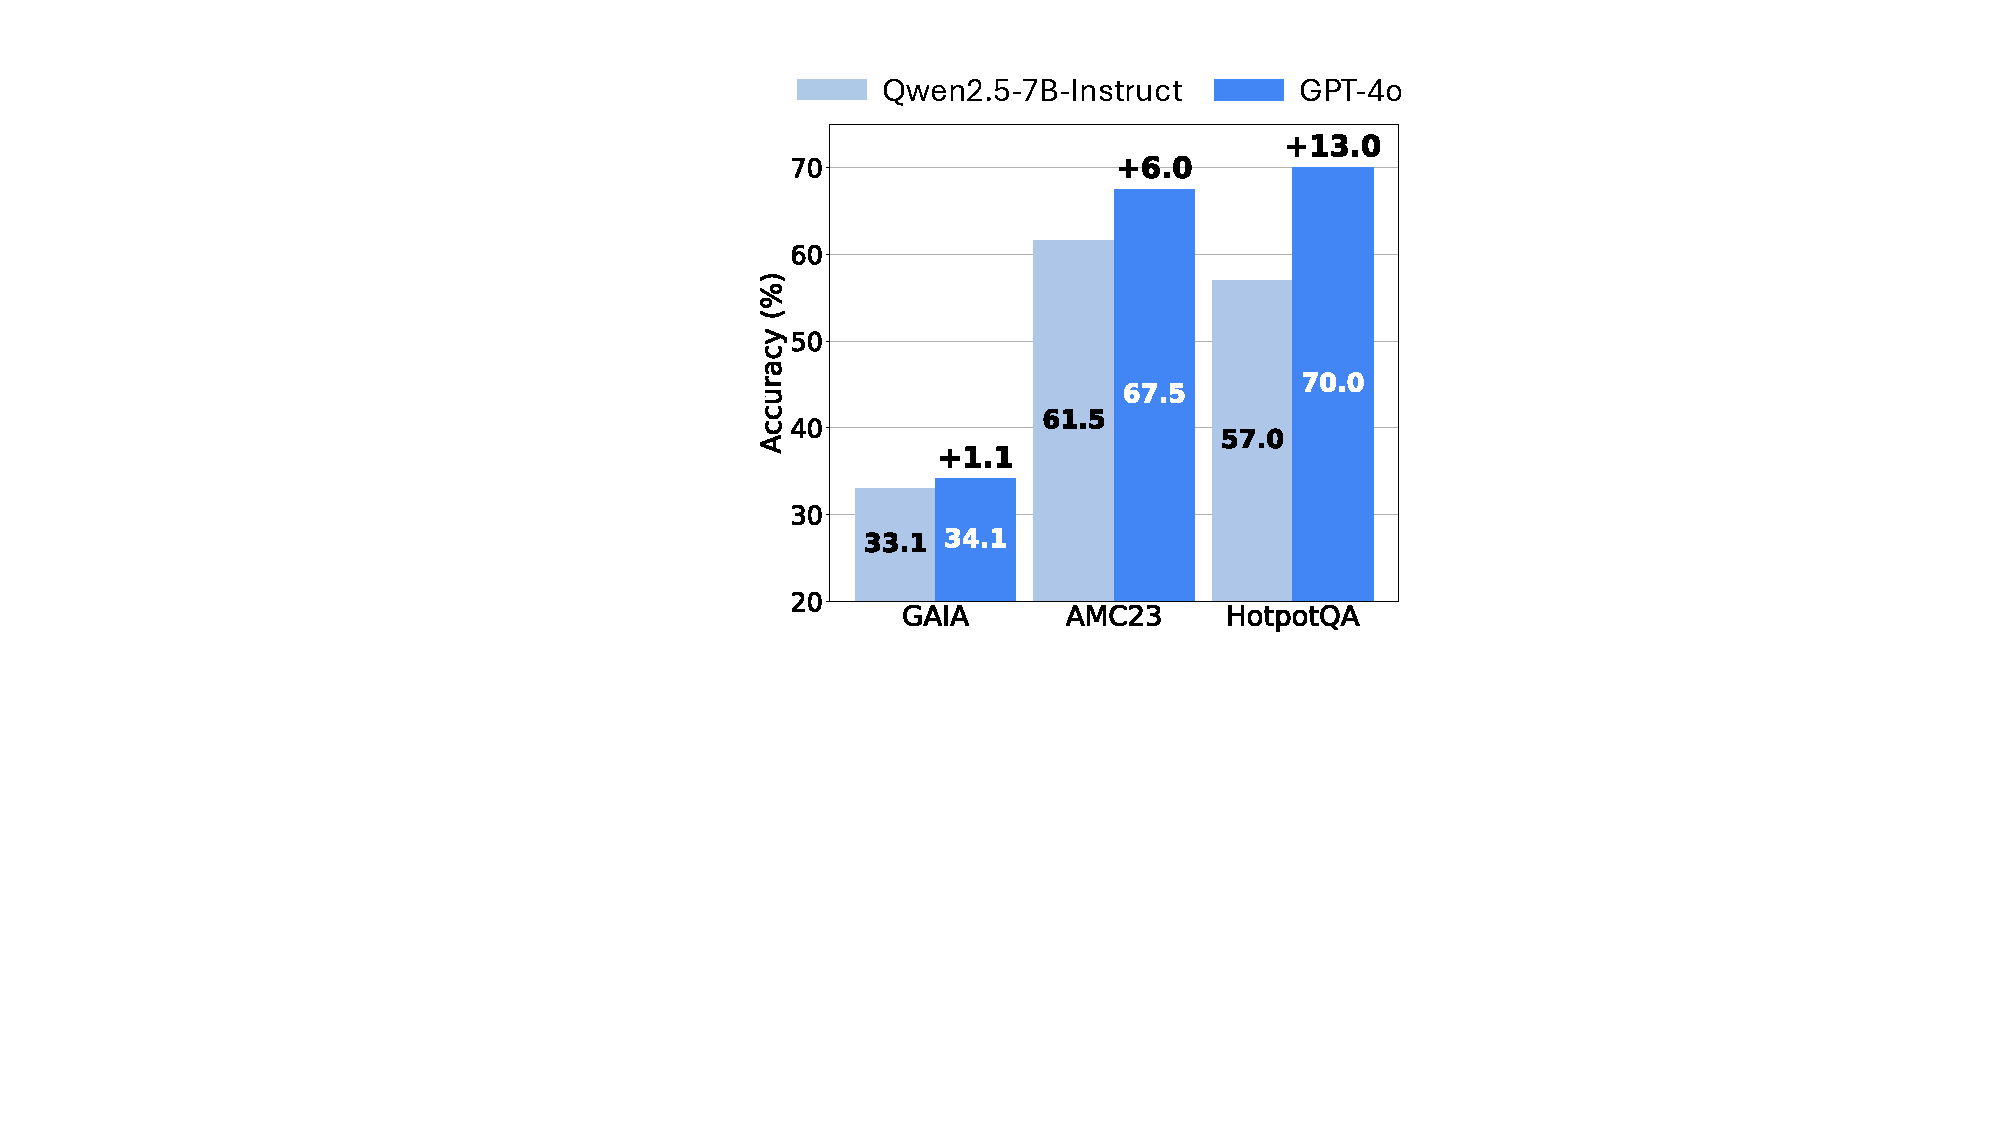
\includegraphics[width=0.7\textwidth]{figs/app_tool_scale.pdf}
    \vspace{-1mm}
    \caption{{\textbf{Tool scaling study}. \model's performance improves when its tools are upgraded from Qwen-2.5-7B-Instruct to GPT-4o.}}
    \label{app:fig:app_tool_scale}
\end{minipage}
\hfill
\begin{minipage}[b]{0.48\textwidth}
    \centering
    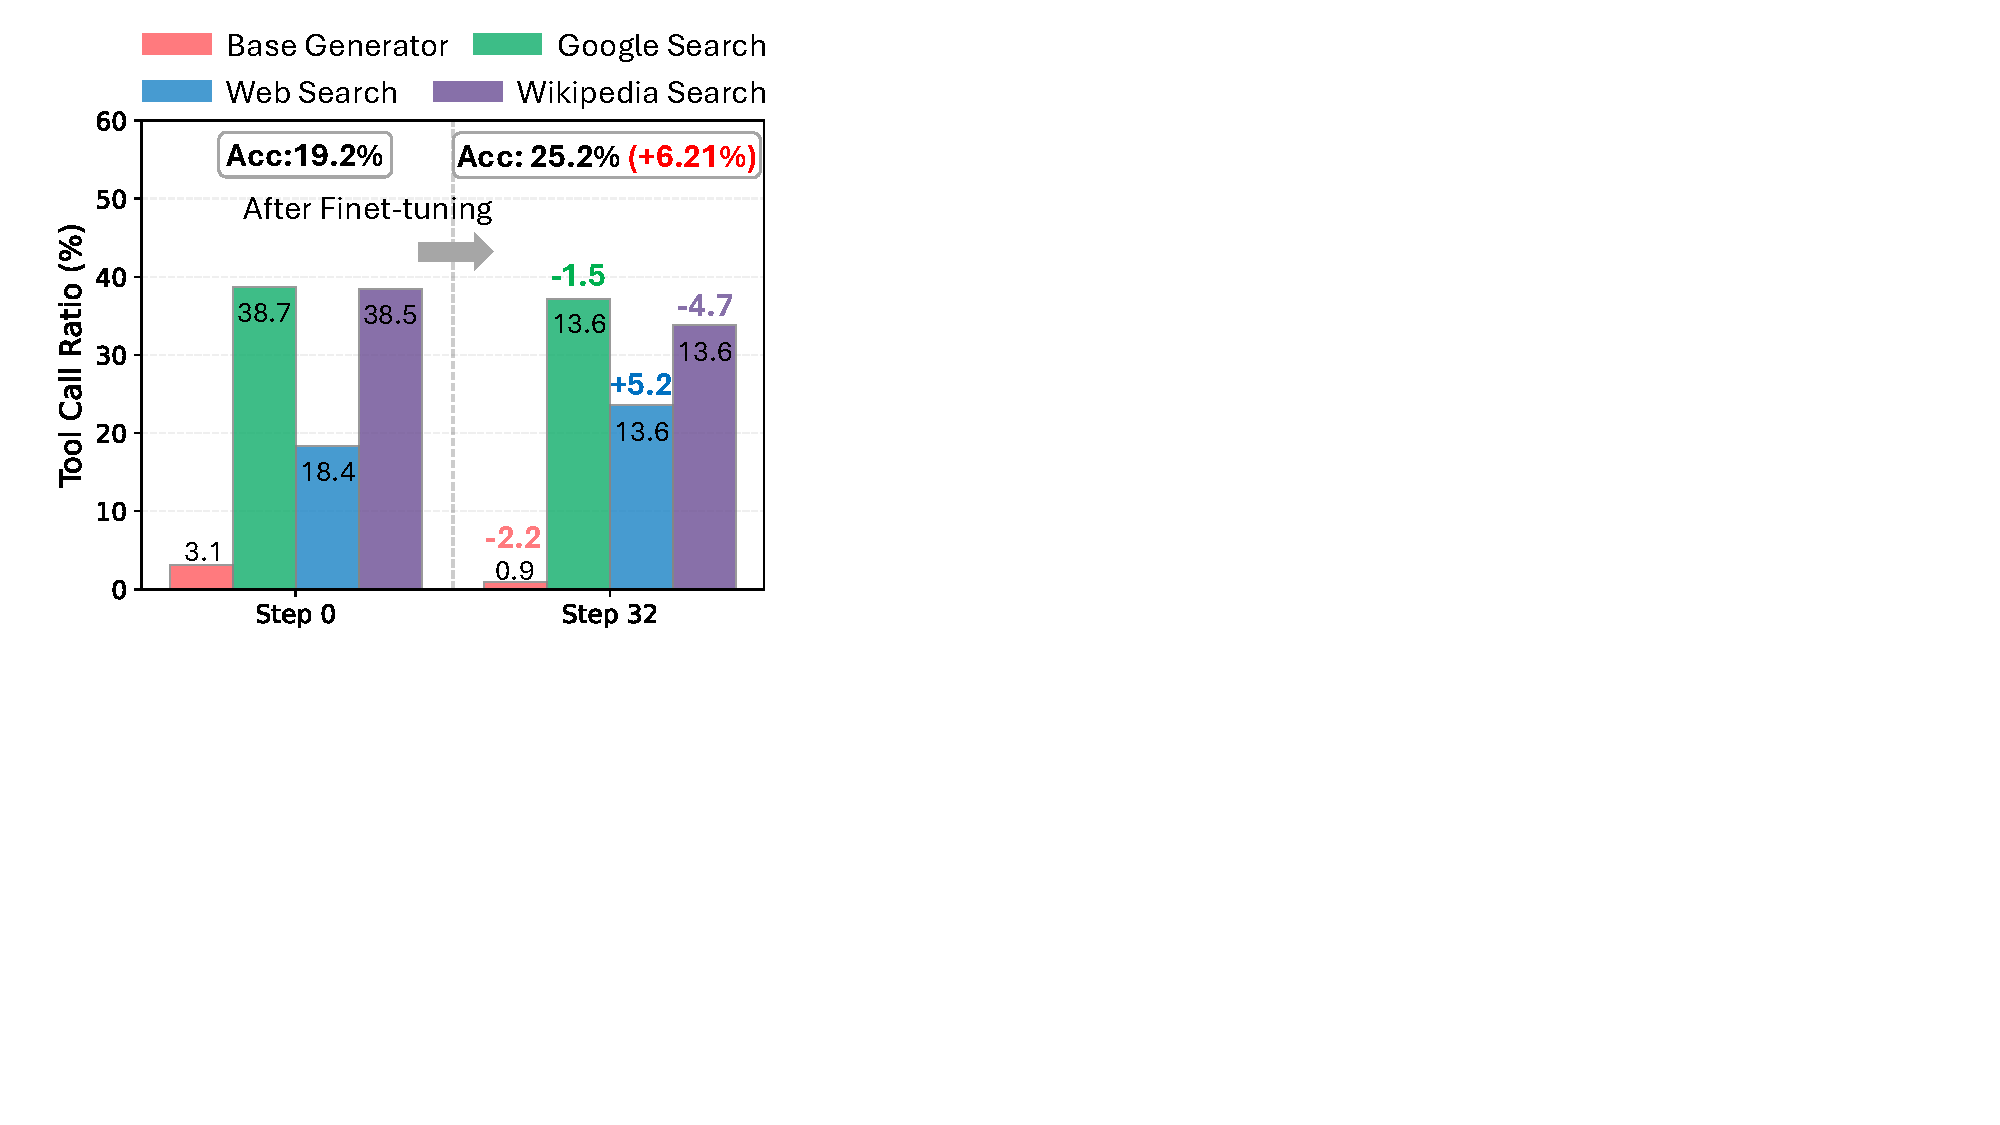
\includegraphics[width=0.75\textwidth]{figs/app_tool_usage.pdf}
    \vspace{-1mm}
    \caption{{\textbf{Tool call optimization on Musique}. \model's planner increases Web Search usage after Flow-GRPO training.}}
    \label{app:fig:app_tool_usage}
\end{minipage}
\end{figure}

\subsection{In-depth Analysis of Optimized Planning}

\paragraph{\model adapts to inference-time tool scaling.}
We scale the tools—the Base Generator and Python Coder—to GPT-4o-powered versions. Empirical results on search and math datasets ({{Figure~\ref{app:fig:app_tool_scale}}}) show that \model, when using these GPT-4o-powered tools, substantially outperforms its performance with Qwen2.5-7B-Instruct-powered tools, achieving improvements of 1.0\% on GAIA, 6.0\% on AMC23, and a notable 13.0\% on HotpotQA. This finding further supports a consistent trend: after in-the-flow RL training, the planner can adaptively leverage improvements in the underlying tools to enhance the agentic system's overall performance.

\paragraph{Flow-GRPO spontaneous tool usage preference change.} 
We further compare tool usage distributions before and after in-the-flow RL training on Musique. {{Figure~\ref{app:fig:app_tool_usage}}} shows that due to Musique's need for a diverse source of information, Flow-GRPO optimizes the planner to increase Web Search to delve deeper into the URL provided by other search tools. This maneuver presents a steady performance improvement of 6.1\%.




\begin{figure}[!ht]
\centering
    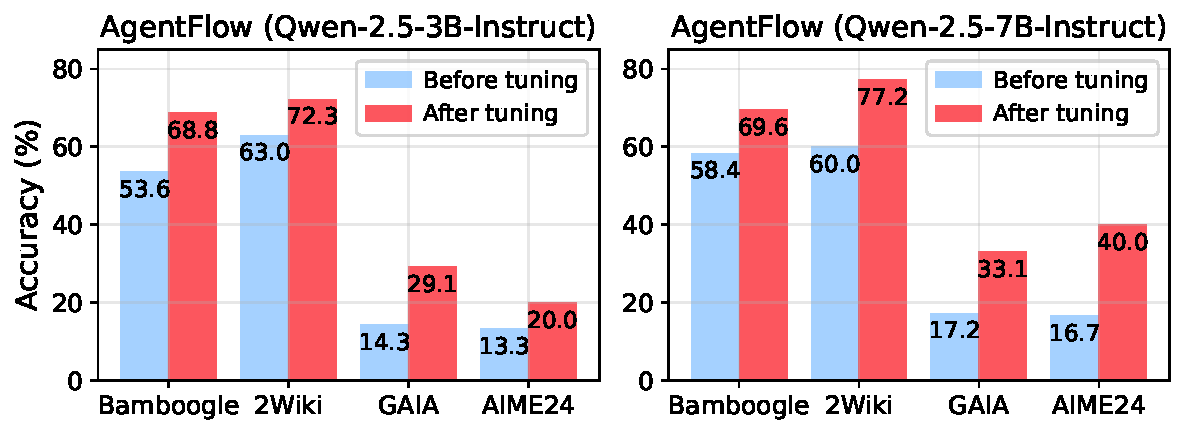
\includegraphics[width=0.85\textwidth]{figs/scaling_model_size.pdf}
    \caption{Flow-GRPO fine-tuning offers consistent gains on \model as the backbone model size scales from 3B to 7B.}
    \label{app:fig:app_scaling_model_size}
\end{figure}

\paragraph{More evidence of training scaling in backbone size.}
We further investigate how the backbone LLM scale affects \model's performance and the efficacy of Flow-GRPO on GameOf24, AMC23, and MedQA. We construct two versions of the system: one using \textit{Qwen2.5-3B-Instruct} and another using \textit{Qwen2.5-7B-Instruct} for all four modules (planner, executor, verifier, and generator) as well as the associated tools. In both versions, only the planner is fine-tuned with Flow-GRPO. As shown in Figure~\ref{app:fig:app_scaling_model_size}, Flow-GRPO fine-tuning consistently improves performance across tasks for both backbones. These results demonstrate that our in-the-flow optimization is effective across model capacities, enhancing \model regardless of LLM size.

\clearpage

\section{Instruction Templates in \model}

\subsection{Modules and Memory}
\label{app:modules_and_memory}

\subsubsection{Action Planner}
\label{app:action_planner}
Tool Metadata can be found in \S\ref{app:tool_metadata}.

\begin{custombox}[title=Instruction for {Action Planner}]{toolcardborder}
\setlength{\parindent}{0pt}
\textbf{Task:} Determine the optimal next step to address the query using available tools and previous context.

\vspace{6pt}
\noindent\textbf{Context:}
\begin{itemize}[left=0pt, label={}, itemsep=0pt, parsep=0pt]
    \item {Query:} {\{{Question}\}}
    \item {Available Tools:} [{Base Generator, Python Coder, Google Search, Wikipedia Search, Web Search}]
    \item {Toolbox Metadata:} [{Tool Metadata1, Tool Metadata2, ...}]
    \item {Previous Steps:} {\{{Actions} {from Memory}\}}
\end{itemize}

\vspace{6pt}
\noindent\textbf{Instructions:}
\begin{enumerate}[left=0pt, itemsep=0pt, parsep=0pt]
    \item Analyze the current objective, the history of executed steps, and the capabilities of the available tools.
    \item Select the {single most appropriate tool} for the next action. 
    \item Consider the {specificity} of the task (e.g., calculation vs. information retrieval).
    \item Consider the {source} of required information (e.g., general knowledge, mathematical computation, a specific URL).
    \item Consider the {limitations} of each tool as defined in the metadata.
    \item Formulate a clear, concise, and achievable {sub-goal} that precisely defines what the selected tool should accomplish.
    \item Provide all necessary {context} (e.g., relevant data, variable names, file paths, or URLs) so the tool can execute its task without ambiguity.
\end{enumerate}

\vspace{6pt}

\noindent\textbf{Response Format:}
\begin{enumerate}[left=0pt, itemsep=0pt, parsep=0pt]
    \item {Justification:} Explain why the chosen tool is optimal for the sub-goal, referencing its capabilities and the task requirements.
    \item {Context:} Provide all prerequisite information for the tool.
    \item {Sub-Goal:} State the exact objective for the tool.
    \item {Tool Name:} State the exact name of the selected tool (e.g., {Wikipedia Search}).
\end{enumerate}

\vspace{6pt}

\noindent\textbf{Rules:}
\begin{itemize}[left=0pt, label={}, itemsep=0pt, parsep=0pt]
    \item Select {only one} tool per step.
    \item The {Sub-Goal} must be directly and solely achievable by the selected tool.
    \item The {Context} section must contain {all} information the tool needs; do not assume implicit knowledge.
    \item The final response must end with the {Context}, {Sub-Goal}, and {Tool Name} sections in that order. No additional text should follow.
\end{itemize}
\end{custombox}

\clearpage
\subsubsection{Tool Executor}
\label{app:tool_executor}
\begin{custombox}[title=Instruction for {Tool Executor}]{toolcardborder}
\textbf{Task:} Generate a precise command to execute the selected tool.

\vspace{6pt}

\noindent\textbf{Context:}
\begin{itemize}[left=0pt, label={}, itemsep=0pt, parsep=0pt]
 \item{Query:} {\{{Question}\}}
    
 \item{Sub-Goal:} {\{{Sub Goal} {from Next Step Plan}\}}
    
 \item{Tool Name:} {\{{Selected Tool} {from Next Step Plan}\}}
    
 \item{Toolbox Metadata:}  \{{{Selected Tool Metadata}} {from Next Step Plan}\}
    
 \item{Relevant Data:} {\{{Context} {from Next Step Plan}\}}
\end{itemize}

\vspace{6pt}

\noindent\textbf{Instructions:}
\begin{enumerate}[left=0pt, itemsep=0pt, parsep=0pt]
    \item Analyze the tool's required parameters from its metadata.
    \item Construct valid Python code that addresses the sub-goal using the provided context and data.
    \item The command must include at least one call to \smalltt{tool.execute()}.
    \item Each \smalltt{tool.execute()} call must be assigned to a variable named {\smalltt{execution}}.
    \item Use exact numbers, strings, and parameters in the \smalltt{tool.execute()} call based on the context.
\end{enumerate}

\vspace{6pt}

\noindent\textbf{Output Format:}
Present your response in the following structured format. Do not include any extra text or explanations.

\vspace{4pt}

\begin{itemize}[left=3pt, label={}, itemsep=0pt, parsep=0pt]
\item \hspace{-3mm}\textbf{Example 1:}\\
Generated Command:
\begin{simplecode}
execution = tool.execute(query="Summarize the following porblom:"Isaac has 100 toys, masa gets ...., how much are their together?")
\end{simplecode}

\item \hspace{-3mm}\textbf{Example 2:}\\
Generated Command:
\begin{simplecode}
execution = tool.execute(query=["Methanol", "function of hyperbola", "Fermat's Last Theorem"])
\end{simplecode}
\end{itemize}
\end{custombox}

\clearpage
\subsubsection{Execution Verifier}
\label{app:execution_verifier}
\begin{custombox}[title=Instruction for {Execution Verifier}]{toolcardborder}
\setlength{\parindent}{0pt}

\textbf{Task:} Evaluate if the current memory is complete and accurate enough to answer the query, or if more tools are needed.

\vspace{6pt}

\noindent\textbf{Context:}

\begin{itemize}[left=0pt, label={}, itemsep=0pt, parsep=0pt]
 \item {Query:} {\{{Question}\}}
    
 \item {Available Tools:} [{Base Generator, Python Coder, Google Search, Wikipedia Search, Web Search}]
    
 \item {Toolbox Metadata:}  [{Tool Metadata1, Tool Metadata2, ...}]
    
 \item {Memory (Tools Used \& Results):} {\{{Actions} {from Memory}\}}
\end{itemize}

\vspace{6pt}

\noindent\textbf{Instructions:}
\begin{enumerate}[left=0pt, itemsep=0pt, parsep=0pt]
    \item Review the original query, the initial analysis, and the complete history of actions and results in the memory.
    \item Does the accumulated information fully address all aspects of the query?
        \item Are there any unanswered sub-questions or missing pieces of information?
    \item Are there any inconsistencies or contradictions between different steps?
        \item Is any information ambiguous, potentially hallucinated, or in need of verification?
    \item Determine if any {unused tools} could provide critical missing information based on their metadata.
\end{enumerate}

\vspace{6pt}

\noindent\textbf{Final Determination:}
\begin{itemize}[left=0pt, label={}, itemsep=0pt, parsep=0pt]
\item If the memory is sufficient to form a complete and accurate answer, explain why and conclude with {``Conclusion: STOP''}.
    
\item If more information is needed, clearly state what is missing, suggest which tool(s) could help, and conclude with {``Conclusion: CONTINUE''}.
\end{itemize}

\vspace{6pt}

\noindent\textbf{Rules:}
\begin{itemize}[left=0pt, label={}, itemsep=0pt, parsep=0pt]
\item The response must end with either {exactly} ``Conclusion: STOP'' or ``Conclusion: CONTINUE''.
    
\item Do not include any text after the conclusion statement.
    
\item Your justification must be concise and directly tied to the query and memory.
\end{itemize}
\end{custombox}


\clearpage
\subsubsection{Solution Generator}
\label{app:solution_generator}
\begin{custombox}[title=Instruction for {Solution Generator}]{toolcardborder}
\setlength{\parindent}{0pt}

\textbf{Task:} Generate a concise final answer to the query based on all provided context.

\vspace{6pt}

\noindent\textbf{Context:}
\begin{itemize}[left=0pt, label={}, itemsep=0pt, parsep=0pt]
 \item {Query:} {\{{Question}\}}
 
 \item {Initial Analysis:} {\{{Query Analysis}\}}
    
 \item {Actions Taken:} {\{{Actions} {from Memory}\}}
\end{itemize}

\vspace{6pt}

\noindent\textbf{Instructions:}
\begin{enumerate}[left=0pt, itemsep=0pt, parsep=0pt]
    \item Carefully review the original user query, the initial analysis, and the complete sequence of actions and their results.
    \item Synthesize the key findings from the action history into a coherent narrative.
    \item Construct a clear, step-by-step summary that explains how each action contributed to solving the query.
    \item Provide a direct, precise, and standalone final answer to the original query.
\end{enumerate}

\vspace{6pt}

\noindent\textbf{Output Structure:}
\begin{enumerate}[left=0pt, itemsep=0pt, parsep=0pt]
    \item {Process Summary:} A clear, step-by-step breakdown of how the query was addressed. For each action, state its purpose (e.g., ``To verify X'') and summarize its key result or finding in one sentence.
    \item {Answer:} A direct and concise final answer to the query. This should be a self-contained statement that fully resolves the user's question.
\end{enumerate}

\vspace{6pt}

\noindent\textbf{Rules:}
\begin{itemize}[left=0pt, label={}, itemsep=0pt, parsep=0pt]
 \item The response must follow the exact two-part structure above.
    
 \item The {Process Summary} should be informative but concise, focusing on the logical flow of the solution.
    
 \item The {Answer} must be placed at the very end and be clearly identifiable.
    
 \item Do not include any additional sections, explanations, or disclaimers beyond the specified structure.
\end{itemize}
\end{custombox}


\clearpage
\subsubsection{Evolving Memory}
\label{app:memory}


\vspace{-1mm}

\begin{custombox}[title=Example {Memory} Entry]{toolcardborder}
\begin{simplecode}
"\textbf{Query}": Where is the largest shopping mall besides Tokyo’s biggest metropolitan station? \\

"\textbf{Action Turn 1}": \{

    \ \ \ \textbf{"Tool Name"}: "Wikipedia Search",
    
    \ \ \  \textbf{"Sub-Goal"}: "Retrieve detailed information about Tokyo‘s metropolitan area from Wikipedia.",
    
    \ \ \ \textbf{"Command"}: "execution = tool.execute(query="Tokyo metropolitan area details")",
    
    \ \ \ \textbf{"Result"}: "The Greater Tokyo Area is the largest metropolitan area in the world...",

    \ \ \  \textbf{"Verification Status"}: "
    
    \ \ \ \ \ \  Brief Review of the Query, Initial Analysis, and Previous Memory.
    
    \ \ \ \ \ \  Assessment of Completeness and Accuracy.
    
    \ \ \ \ \ \ Conclusion: The memory is not complete and accurate enough to answer the query. Additional tools are needed to verify or generate more solutions.
    
    \ \ \ \ \ \  \textbf{Final Determination:} \textbf{CONTINUE}"
    
\},\\

"\textbf{Action Turn 2}": \{

\ \ \ \ ...

\},\\

...\\

"\textbf{Action Turn t}": \{

\ \ \ \ ...

\ \ \  \textbf{"Verification Status"}: "
    
    \ \ \ \ \ \ Brief Review of the Query, Initial Analysis, and Previous Memory.
    
    \ \ \ \ \ \  Assessment of Completeness and Accuracy. (Including Time Dilation Calculation, Geographic Precise, Inconsistencies or Contradictions, Unit Conversion, etc. )
    
    \ \ \ \ \ \ Conclusion: The memory is complete and accurate enough to answer the query. No additional tools are needed to verify or generate more solutions.
    
    \ \ \ \ \ \  \textbf{Final Determination:} \textbf{STOP}"
\\\}
\end{simplecode}
\end{custombox}


Our shared evolving memory system creates a deterministic, structured record that captures the reasoning process across three integrated agents: the \textit{Action Planner}, \textit{Tool Executor}, and \textit{Execution Verifier}. By sequentially stacking crucial information from each action step, the system enables transparent state tracking, controllable behavior, and bounded context growth.

The memory reading and matching process employs regular expressions to parse outputs generated by different system components, adhering to standardized formats defined in their respective component instructions. For the \textit{Action Planner}, we use a relatively permissive regular expression to extract key information. Specifically, it matches the content immediately following: \textit{Sub-Goal} as the sub-goal and the content following; \textit{Tool Name} as the selected tool. This extracted information is then used to populate the next memory entry. For the \textit{Tool Executor}, the regular expression is designed to capture the entire \textit{Command} line starting with \texttt{execution = tool.execute(...)}. Additionally, the value passed to the \textit{Query} parameter within this command is parsed and saved into the memory for future reference. All results returned by the tools are directly stored in the \textit{Result} field of the memory. The \textit{Verification Status} is extracted from \textit{Execution Verifier}, including a brief analysis of the current tool result and previous memory, and then it gives a conclusion whether the loop needs to be CONTINUE or STOP.
\vspace{-2mm}


\clearpage
\subsection{Toolset Metadata}
\label{app:tool_metadata}
This section details the implementation and metadata of the tools used in our main results.  We employ a suite of specialized tools, each designed for distinct tasks. Below, we present core metadata for each tool, including its functionality, input/output schema, limitations, and best practices.

\subsubsection{Base Generator}
\begin{tooldescbox}{{Base Generator}}
\setlength{\parindent}{0pt}
\setlength{\parskip}{4pt}

\textbf{Description:} A generalized tool that takes query from the user, and answers the question step by step to the best of its ability. It can also accept an image.

\vspace{6pt}

\inputtype{query: str - The query that includes query from the user to guide the agent to generate response.}

\vspace{4pt}

\outputtype{str - The generated response to the original query}

\vspace{6pt}

\textbf{Demo Commands:}
\begin{itemize}[left=0pt, label={}, itemsep=0pt, parsep=0pt]
\item \textbf{Command:}
\begin{simplecode}
\texttt{execution = tool.execute(query="Summarize the following text in a few lines")}
\end{simplecode}

 \text{Description:} Generate a short summary given the query from the user.
\end{itemize}
\begin{limitationbox}
The Base Generator may provide hallucinated or incorrect responses.
\end{limitationbox}

\begin{bestpracticebox}
\begin{toolenum}
    \item Use it for general queries or tasks that don't require specialized knowledge or specific tools in the toolbox.
    \item Provide clear, specific query.
    \item Use it to answer the original query through step by step reasoning for tasks without complex or multi-step reasoning.
    \item For complex queries, break them down into subtasks and use the tool multiple times.
    \item Use it as a starting point for complex tasks, then refine with specialized tools.
    \item Verify important information from its responses.
\end{toolenum}
\end{bestpracticebox}

\textbf{LLM Engine Required:} True
\end{tooldescbox}

\clearpage
\subsubsection{Python Coder}



\begin{tooldescbox}{{Python Coder}}
\setlength{\parindent}{0pt}
\setlength{\parskip}{4pt}

\textbf{Description:} A tool that generates and executes simple Python code snippets for basic arithmetical calculations and math-related problems. The generated code runs in a highly restricted environment with only basic mathematical operations available.

\vspace{6pt}

\inputtype{query: str - A clear, specific description of the arithmetic calculation or math problem to be solved, including any necessary numerical inputs.}

\vspace{4pt}

\outputtype{dict - A dictionary containing the generated code, calculation result, and any error messages.}

\textbf{Output prompt:} Given a query, generate a Python code snippet that performs the specified operation on the provided data. Please think step by step. Ensure to break down the process into clear, logical steps. Make sure to print the final result in the generated code snippet with a descriptive message explaining what the output represents. The final output should be presented in the following format:
\begin{simplecode}
{\verb|```| python

<code snippet>

\verb|```| }
\end{simplecode}

\vspace{6pt}

\textbf{Demo Commands:}
\begin{itemize}[left=0pt, label={}, itemsep=0pt, parsep=0pt]
\item \textbf{Command:} 

\begin{simplecode}
{execution = tool.execute(query="Find the sum of prime numbers up to 50")}
\end{simplecode}

\enspace\text{Description:} Generate a Python code snippet to find the sum of prime numbers up to 50.
    
\vspace{4pt}
    
\item \textbf{Command:} 
\begin{simplecode}
{{query=" Given the list [1, 2, 3, 4, 5, 6, 7, 8, 9, 10], calculate the sum of squares of odd numbers”\\
execution = tool.execute(query=query)}}
\end{simplecode}
    
\enspace\text{Description:} Generate a Python function for a mathematical operation on a given list of numbers.
\end{itemize}

\begin{limitationbox}
\begin{toolenum}
    \item Restricted to basic Python arithmetic operations and built-in mathematical functions.
    \item Cannot use any external libraries or modules, including those in the Python standard library.
    \item Limited to simple mathematical calculations and problems.
    \item Cannot perform any string processing, data structure manipulation, or complex algorithms.
    \item No access to any system resources, file operations, or network requests.
    \item Cannot use `import' statements.
    \item All calculations must be self-contained within a single function or script.
    \item Input must be provided directly in the query string.
    \item Output is limited to numerical results or simple lists/tuples of numbers.
    \item Output should be kept to a single numerical result or a simple list/tuple of numbers.
    \item DO NOT generate loop output.
\end{toolenum}
\end{limitationbox}

\begin{bestpracticebox}
\begin{toolenum}
    \item Provide clear and specific queries that describe the desired mathematical calculation.
    \item Include all necessary numerical inputs directly in the query string.
    \item Keep tasks focused on basic arithmetic, algebraic calculations, or simple algorithms.
    \item Ensure all required numerical data is included in the query.
    \item Verify that the query only involves mathematical operations and does not require any data processing or complex algorithms.
    \item Review generated code to ensure it only uses basic Python arithmetic operations and built-in math functions.
\end{toolenum}
\end{bestpracticebox}

\textbf{LLM Engine Required:} True
\end{tooldescbox}

\clearpage
\subsubsection{Google Search}
\begin{tooldescbox}{{Google Search}}
\setlength{\parindent}{0pt}
\setlength{\parskip}{4pt}

\textbf{Description:} A web search tool powered by Google Search that provides real-time information from the internet with citation support.

\vspace{6pt}

\inputtype{query: str - The search query to find information on the web.}

\vspace{4pt}

\inputtype{add\_citations: bool - Whether to add citations to the results. If True, the results will be formatted with citations. By default, it is True.}

\vspace{4pt}

\outputtype{str - The search results of the query.}

\vspace{6pt}

\textbf{Demo Commands:}
\begin{itemize}[left=0pt, label={}, itemsep=0pt, parsep=0pt]
\item \textbf{Command:} 
\begin{simplecode}
{{execution = tool.execute(query="What is the capital of France?")}}
\end{simplecode}

    \enspace\text{Description:} Search for general information about the capital of France with default citations enabled.
    
    \vspace{4pt}
    

    \item \textbf{Command:} 
    \begin{simplecode}
    {{execution = tool.execute(query="Who won the euro 2024?", add\_citations=False)}}
    \end{simplecode}

    \enspace\text{Description:} Search for information about the Euro 2024 winner without citations.
    
    \vspace{4pt}
    

    \item \textbf{Command:} 
    \begin{simplecode}
    {{execution = tool.execute(query="Physics and Society article arXiv August 11, 2016”, add\_citations=True)}}
    \end{simplecode}

    \enspace\text{Description:} Search for specific academic articles with citations enabled.
\end{itemize}
\begin{limitationbox}
\begin{toolenum}
    \item This tool is only suitable for general information search.
    \item This tool contains less domain-specific information.
    \item This tool is not suitable for searching and analyzing videos on YouTube or other video platforms.
\end{toolenum}
\end{limitationbox}

\begin{bestpracticebox}
\begin{toolenum}
    \item Choose this tool when you want to search for general information about a topic.
    \item Choose this tool for question types of query, such as ``What is the capital of France?'' or ``Who invented the telephone?''.
    \item The tool will return summarized information.
    \item This tool is more suitable for definition, world knowledge, and general information search.
\end{toolenum}
\end{bestpracticebox}

\textbf{LLM Engine Required:} False
\end{tooldescbox}


\clearpage
\subsubsection{Wikipedia Search}
Wikipedia search will first call Wikipedia API to retrieve relevant URLs with snippets. Then the RAG (Retrieval-Augmented Generation) process begins by extracting raw text content from the given webpage URL, cleaning it to remove HTML elements and retain only meaningful text. This content is then split into overlapping chunks of approximately 200 words each, with a 20-word overlap to preserve context across segments from the first 1M words in each URL. Next, both the user's query and the document chunks are embedded into the vector space using the OpenAI \texttt{text-embedding-3-small\footnote{\url{https://platform.openai.com/docs/models/text-embedding-3-small}}} model. The system computes the cosine similarity between the query embedding and each chunk embedding to rank the chunks by relevance. We set that the top 10 most similar chunks are selected and passed forward as context. And a base LLM engine will summarize the extracted context. 

Wikipedia search will first call Wikipedia API to retrieve relevant URLs with snippets. 

\begin{tooldescbox}{{Wikipedia Search}}
\setlength{\parindent}{0pt}

\text{Description:} A tool that searches Wikipedia and returns relevant pages with their page titles, URLs, abstract, and retrieved information based on a given query.

\vspace{6pt}

\inputtype{query: str - The search query for Wikipedia.}

\vspace{4pt}

\outputtype{dict - A dictionary containing search results, all matching pages with their content, URLs, and metadata.}

\vspace{6pt}

\textbf{Demo Commands:}
\begin{itemize}[left=0pt, label={}, itemsep=0pt, parsep=0pt]
\item \textbf{Command:} 
\begin{simplecode}{{execution = tool.execute(query="What is the exact mass in kg of the moon")}}
\end{simplecode}

   \item \text{Description:} Search Wikipedia and get the information about the mass of the moon.
    
    \vspace{4pt}
    
    \item \textbf{Command:} 
    \begin{simplecode}
    {{execution = tool.execute(query="Funtion of human kidney")}}
    \end{simplecode}
    
    \text{Description:} Search Wikipedia and get the information about the function of the human kidney.
    
    \vspace{4pt}
    
    \item \textbf{Command:}  
    \begin{simplecode}
    {{execution = tool.execute(query="When was the first moon landing?")}}
    \end{simplecode}
    
    \text{Description:} Search Wikipedia and get the information about the first moon landing.
\end{itemize}
\begin{limitationbox}
\begin{toolenum}
    \item It is designed specifically for retrieving grounded information from Wikipedia pages only.
    \item The returned information accuracy depends on Wikipedia's content quality.
\end{toolenum}
\end{limitationbox}

\begin{bestpracticebox}
\begin{toolenum}
    \item Use specific, targeted queries rather than broad or ambiguous questions.
    \item If initial results are insufficient, examine the ``other\_pages'' section for additional potentially relevant content.
    \item Use this tool as part of a multi-step research process rather than a single source of truth.
    \item You can use the Web Search to get more information from the URLs.
\end{toolenum}
\end{bestpracticebox}

\textbf{LLM Engine Required:} True
\end{tooldescbox}

\clearpage
\subsubsection{Web Search}
Web search will directly access the URL in the query. Then the RAG (Retrieval-Augmented Generation) process begins by splitting content from the page into overlapping chunks of approximately 200 words each, with a 20-word overlap to preserve context across segments from the first 1M words in each URL. Next, both the user's query and the document chunks are embedded into the vector space using the OpenAI {text-embedding-3-small\footnote{\url{https://platform.openai.com/docs/models/text-embedding-3-small}}} model. The system computes the cosine similarity between the query embedding and each chunk embedding to rank the chunks by relevance. We set that the top 10 most similar chunks are selected and passed forward as context. And a base LLM engine will summarize the extracted context. 

\begin{tooldescbox}{{Web Search}}
\setlength{\parindent}{0pt}

\textbf{Description:} A specialized tool for answering questions by retrieving relevant information from a given website using RAG (Retrieval-Augmented Generation).

\vspace{6pt}

\inputtype{query: str - The search query for the website.}

\vspace{4pt}

\inputtype{url: str - The URL of the website to retrieve information from.}

\vspace{4pt}

\outputtype{str - The answer to the user's query based on the information gathered from the website.}

\vspace{6pt}

\textbf{Demo Commands:}
\begin{itemize}[left=0pt, label={}, itemsep=0pt, parsep=0pt]
\item \textbf{Command:} 
\begin{simplecode}
{{execution = tool.execute(query="What is the exact mass in kg of the moon?", url="https://en.wikipedia.org/wiki/Moon")}}
\end{simplecode}

    \enspace\text{Description:} Retrieve information about the moon's mass from Wikipedia.
    
    \vspace{4pt}
    
    \item \textbf{Command:} 
    \begin{simplecode}
    {{execution = tool.execute(query="What are the main features of Python programming language?", url="https://www.python.org/about/apps/")}}
    \end{simplecode}

    \enspace\text{Description:} Get information about Python features from the official website.
\end{itemize}
\begin{limitationbox}
\begin{toolenum}
    \item Requires valid URLs that are accessible and contain text content.
    \item May not work with JavaScript-heavy websites or those requiring authentication.
    \item Performance depends on the quality and relevance of the website content.
    \item May return incomplete or inaccurate information if the website content is not comprehensive.
    \item Limited by the chunking and embedding process which may miss context.
    \item Requires OpenAI API access for embeddings and LLM generation.
\end{toolenum}
\end{limitationbox}

\begin{bestpracticebox}
\begin{toolenum}
    \item Use specific, targeted queries rather than broad questions.
    \item Ensure the URL is accessible and contains relevant information.
    \item Prefer websites with well-structured, text-rich content.
    \item For complex queries, break them down into smaller, specific questions.
    \item Verify important information from multiple sources when possible.
    \item Use it as part of a multi-step research process rather than a single source of truth.
    \item It is highly recommended to use this tool after calling other web-based tools (e.g., Google Search, Wikipedia Search, etc.) to get the real, accessible URLs.
\end{toolenum}
\end{bestpracticebox}

\textbf{LLM Engine Required:} True
\end{tooldescbox}

\clearpage
\subsection{LLM-based Judging}
\label{app:llm_based_judging}
We employ GPT-4o as our judge model using a two-step ``analyze-then-judge'' instruction paradigm to ensure both accuracy and efficiency.

\begin{custombox}[title=Reward Function Instruction in Training]{toolcardborder}
\setlength{\parindent}{0pt}

\textbf{Task:} Determine if the Model Response is equivalent to the Ground Truth.

\vspace{6pt}

\noindent\textbf{Instructions:}
\begin{enumerate}[left=0pt]
    \item \textbf{Extract:} Isolate the final answer from the Model Response, ignoring all reasoning steps. Look specifically for content within \boxed{...} or the concluding statement.
    \item \textbf{Normalize \& Compare:} Assess equivalence after normalization:
    \item \textbf{Mathematical Answers:} Must be mathematically identical (e.g., $\frac{1}{2}$ is equivalent to $0.5$).
        \item \textbf{Numerical/Textual Answers:} Ignore formatting (commas, spaces), case sensitivity, and extraneous units/currency (e.g., ``1,000'' == ``1000'', ``Paris'' == ``PARIS'').
        \item \textbf{Multiple Choice Questions (MCQ):} The answer must match either the correct option's content (e.g., ``Paris'') or its identifier (e.g., ``A'' or ``1st'').
    \item \textbf{Verdict:} Return ``True'' only if the normalized answers are semantically or mathematically equivalent.
\end{enumerate}

\vspace{6pt}

\noindent\textbf{Inputs:}
\begin{itemize}[left=0pt, label={}, itemsep=0pt, parsep=0pt]
\item {Question:} {\{{Question}\}}

    \item {Model Response:} {\{{Final Response} {from Solution Generator}\}}

   \item {Ground Truth:} {\{{GT}\}}
\end{itemize}

\vspace{6pt}

\noindent\textbf{Output Format:}
Present your response in the following structured format. Do not include any extra text or explanations.
\textless{}\texttt{analysis}\textgreater{}: Brief analysis of the comparison.\\
\textless{}\texttt{true\_false}\textgreater{}: ``True'' or ``False''.
\end{custombox}


\clearpage
\section{Case Studies}
\label{app:case_studies}
In this section, we conduct a case study to demonstrate how our \model, coherent with Flow-GRPO, enhances problem-solving performance with greater elegance, efficiency, and robustness. We present solution comparisons showing brief outputs from memory of the \textit{Action Planner} (Qwen2.5-7B-Instruct) before (w/o) tuning by Flow-GRPO and after (w/) Flow-GRPO tuning, with the methodology detailed in \S\ref{subsec:flow-grpo}.


\subsection{Example 1: Efficient Search for Simple Tasks}
\label{case1_gameof24_3B}
This case demonstrates that, with Flow-GRPO tuning, the \textit{Action Planner} can effectively leverage the search engine to retrieve correct answers for simple tasks in a highly efficient manner—unlike the untuned baseline, which requires multiple trials.

\begin{custombox}[title=Example from \# GameOf24]{toolcardborder}
\textbf{Question:} Using the numbers [1, 1, 1, 13], create an expression that equals 24. You must use basic arithmetic operations (+, -, *, /) and parentheses.

\vspace{1em}

\textbf{Answer:} (13-1)*(1+1)
\end{custombox}

\begin{small}
\begin{center}

    \begin{casebox}{successbg}{successframe}{Success Case: \model w/ Flow-GRPO}
    \textbf{Action Step 1:}
    \begin{itemize}[nosep, leftmargin=*]
        \item \textbf{Tool:} \smalltt{Google Search}
        \item \textbf{Sub-goal:} Find a valid arithmetic expression that equals 24 using the numbers [1, 1, 1, 13].
        \item \textbf{Command:} 
        
        \smalltt{tool.execute(query="[1, 1, 1, 13] arithmetic expression to get 24")}
        \item \textbf{Result:} Here's an arithmetic expression using the numbers 1, 1, 1, and 13 to get 24: (13 - 1) * (1 + 1) = 24
    \end{itemize}

    \vspace{1em}

    \textbf{Execution Verifier:} \textcolor{successframe}{PASS, STOP}

    \vspace{1em}

    \textbf{Solution Generator: }\textcolor{successframe}{The arithmetic expression is $((13 - 1) \times (1 + 1)) = 24$.}
    
\end{casebox}

\begin{casebox}{failbg}{failframe}{Failure Case: \model w/o Flow-GRPO}
    \textbf{Action Step 1:}
    \begin{itemize}[nosep, leftmargin=*]
        \item \textbf{Tool:} \smalltt{Python Coder}
        \item \textbf{Sub-goal:} Generate and test all possible combinations of the numbers [1, 1, 1, 13] using basic arithmetic operations and parentheses to find an expression that equals 24.
        \item \textbf{Command:} 
        
        \smalltt{tool.execute(query="[1, 1, 1, 13] execution = (1 * (13 - 1 - 1))")}
        \item \textbf{Result:}
        \begin{casecode}{failbg}
        
            \# Define the values
            
            value\_list = [1, 1, 1, 13]
            
            operation\_result = 1 * (13 - 1 - 1)
            
            \# Print the result with a descriptive message
            
            print(f"The result of the operation is: {operation\_result}")
        \end{casecode}
        The result of the operation is: 11
    \end{itemize}

    \vspace{1em}

    \textbf{Action Step 2:}
    \begin{itemize}[nosep, leftmargin=*]
        \item \textbf{Tool:} \smalltt{Python Coder}
        \item \textbf{Sub-goal:} Generate and test all possible combinations of the numbers [1, 1, 1, 13] using basic arithmetic operations and parentheses to find an expression that equals 24.
        \item \textbf{Command:}
        
        \smalltt{tool.execute(query="[1, 1, 1, 13] -> ((1 + 1 + 1) * 13)")}
        \item \textbf{Result:} \textcolor{red}{Error: unexpected indent ($<$string$>$, line 2)}.
    \end{itemize}

    \vspace{1em}


    \textbf{Action Steps 3-8:}
    \begin{itemize}[nosep, leftmargin=*]
        \item \textbf{Tool:} \smalltt{No matched tool given} \textcolor{red}{\textbf{(Tool Not Found)}}
        \item \textbf{Sub-goal:} Generate and test all possible combinations of the numbers [1, 1, 1, 13] using basic arithmetic operations and parentheses to find an expression that equals 24.
        \item \textbf{Command:} Not command is generated due to the tool not found.
        \item \textbf{Result:} Not result is generated due to the tool not found.
        \item \textit{Note: These steps are identical repetitions where the agent failed to find a matching tool.}
    \end{itemize}

    \vspace{1em}

    
    \textbf{Execution Verifier:} \textcolor{red}{STOP, Tool Not Found}
    
    \vspace{1em}

    
    \textbf{Solution Generator: } \textcolor{red}{The agent incorrectly concludes that $(1 + 1 + 1) \times 13 = 24$.}
    
\end{casebox}

\end{center}
\end{small}


\subsection{Example 2: Spontaneous Brute-force}
\label{case2_gameof24_7B}
This case demonstrates that, when tuned with Flow-GRPO, the \textit{Action Planner} first attempts several solutions, recognizes their ineffectiveness, resorts to a brute-force approach, and finally verifies the result using a search engine.

\begin{custombox}[title=Example from \# GameOf24]{toolcardborder}
\textbf{Question:} Using the numbers [1, 1, 6, 9], create an expression that equals 24. You must use basic arithmetic operations (+, -, *, /) and parentheses.

\vspace{1em}

\textbf{Answer:} (1+1)*9+6
\end{custombox}

\begin{small}
\begin{center}

\begin{casebox}{successbg}{successframe}{Success Case: \model w/ Flow-GRPO}
    \textbf{Action Step 1: Initial Attempt}
    \begin{itemize}[nosep, leftmargin=*]
        \item \textbf{Tool:} \smalltt{Python Coder}
        \item \textbf{Sub-goal:} Generate and test all possible arithmetic expressions using the numbers [1, 1, 6, 9] exactly once to check if any combination equals 24.
        \item \textbf{Command:} 
        
        \smalltt{tool.execute(query="Using the numbers [1, 1, 6, 9], create an expression that equals 24 using basic arithmetic operations and parentheses.")}
        \item \textbf{Result:}
        \begin{casecode}{successbg}
\# Given numbers

numbers = [1, 1, 6, 9]

\# Calculate the expression

result = (numbers[0] + numbers[1]) * (numbers[3] - numbers[2])

\# Print the result

print(f"The result of the expression ({numbers[0]} + {numbers[1]} ) * ({numbers[3]} - {numbers[2]}) is: {result}")
        \end{casecode}
        The result of the expression (1 + 1 ) * (9 - 6) is: 6
    \end{itemize}

    \vspace{1em}

    \textbf{Action Step 2: Tool Error}
    \begin{itemize}[nosep, leftmargin=*]
        \item \textbf{Tool:} \smalltt{Python Coder}
        \item \textbf{Sub-goal:} Generate and test all possible permutations of the numbers with different operator placements to find an expression that equals 24.
        \item \textbf{Command:} 
        
        \smalltt{tool.execute(query="Using the numbers [1, 1, 6, 9], create an expression with +,-,*,/ that equals 24")}
        \item \textbf{Result:} \textcolor{orange}{Error: eval() arg 1 must be a string, bytes or code object}
    \end{itemize}

    \vspace{1em}

    \textbf{Action Step 3: Second Attempt}
    \begin{itemize}[nosep, leftmargin=*]
        \item \textbf{Tool:} \smalltt{Python Coder}
        \item \textbf{Sub-goal:} Generate all possible combinations of the four numbers with every permutation of operators (+,-,*,/) to find a valid equation resulting in exactly 24.
        \item \textbf{Command:} 
        
        \smalltt{tool.execute(query="Using the numbers [1, 1, 6, 9] create an expression with +,-,*,/ that equals to '24'")}
        \item \textbf{Result:}
        \begin{casecode}{successbg}
\# Given numbers

numbers = [1, 1, 6, 9]
        \end{casecode}
        \begin{casecode}{successbg}
\# Calculate the expression

result = (numbers[2] - numbers[0]) * (numbers[3] / numbers[1]) / numbers[1]

\# Print the result

print(f"The result of the expression is: {result}")
        \end{casecode}
        The result of the expression is: 45.0
    \end{itemize}

    \vspace{1em}

    \textbf{Action Step 4: Systematic Search (Breakthrough)}
    \begin{itemize}[nosep, leftmargin=*]
        \item \textbf{Tool:} \smalltt{Python Coder}
        \item \textbf{Sub-goal:} Generate and evaluate all possible permutations of the four numbers with every permutation of operators (+,-,*,/) to find a valid equation resulting in exactly 24.
        \item \textbf{Command:} 
        
        \smalltt{tool.execute(query="Using the numbers [1, 1, 6, 9] create an expression that equals 24 using +,-,/,*")}
        \item \textbf{Result:} \textbf{Successfully found valid expressions:} The expression (1+1)*9+6 equals 24. The expression 6+(1+1)*9 equals 24. The expression 6+(9*(1+1)) equals 24. The expression 9*(1+1)+6 equals 24.
    \end{itemize}

    \vspace{1em}

    \textbf{Action Step 5: Confused Verification}
    \begin{itemize}[nosep, leftmargin=*]
        \item \textbf{Tool:} \smalltt{Python Coder}
        \item \textbf{Sub-goal:} Simplify and verify if any minor adjustments to the existing promising expression can achieve an exact match of 24.
        \item \textbf{Command:} 
        
        \smalltt{tool.execute(query="Using the numbers [1, 1, 6, 9] and basic arithmetic operations create an expression that equals 24: (9 * (6 * (1 + 1)))")}
        \item \textbf{Result:} \textcolor{orange}{The result of the expression (9 * (1 + 1) * 6) is: 108}
    \end{itemize}

    \vspace{1em}

    \textbf{Action Step 6: Final Verification}
    \begin{itemize}[nosep, leftmargin=*]
        \item \textbf{Tool:} \smalltt{Google Search}
        \item \textbf{Sub-goal:} Search online for examples or discussions related to creating expressions using given numbers that equal a target value.
        \item \textbf{Command:} 
        
        \smalltt{tool.execute(query="using the numbers [1, 1, 6, 9] create an expression that equals 24", add\_citations=True)}
        \item \textbf{Result:} Here's an expression using the numbers that equals 24: (1 + 1) * 9 + 6 = 24
    \end{itemize}

    \vspace{1em}

    \textbf{Execution Verifier:} \textcolor{successframe}{PASS, STOP (via exhaustive search and verification)}

    \vspace{1em}

    \textbf{Solution Generator: } \textcolor{successframe}{After a multi-step process of trial, error, and verification, the final correct expression is \textbf{(1 + 1) * 9 + 6 = 24}.}

\end{casebox}

\begin{casebox}{failbg}{failframe}{Failure Case: \model w/o Flow-GRPO}
    \textbf{Action Step 1:}
    \begin{itemize}[nosep, leftmargin=*]
        \item \textbf{Tool:} \smalltt{Python Coder}
        \item \textbf{Sub-goal:} Generate and test Python code snippets to find an arithmetic expression using the numbers [1, 1, 6, 9] exactly once that equals 24.
        \item \textbf{Command:} 
        
        \smalltt{tool.execute(query="Using the numbers [1, 1, 6, 9], create an expression that equals 24 using basic arithmetic operations and parentheses.")}
        \item \textbf{Result:}
        \begin{casecode}{failbg}
\# Define the numbers

numbers = [1, 1, 6, 9]

\# Calculate the expression

result = (6 * 9) - ((1 + 1) * 15)

\# Print the result with a descriptive message

print("The result of the expression is:", result)
        \end{casecode}
        The result of the expression is: 24
    \end{itemize}

    \vspace{1em}

    \textbf{Execution Verifier:} \textcolor{red}{STOP}

    \vspace{1em}

    \textbf{Solution Generator: } \textcolor{red}{The agent incorrectly concludes the answer is $(6 \times 9) - ((1 + 1) \times 15)$, failing to notice it used the number \textbf{15}, which was not in the allowed input set.}
\end{casebox}


\end{center}
\end{small}


\clearpage
\subsection{Example 3: A Good Initial Plan is Essential}
\label{case3_gaia_1}
This case demonstrates that a well-crafted initial search with a highly relevant query is far more effective than issuing numerous wrong paths. When tuned with Flow-GRPO, the \textit{Action Planner} in \model can identify the optimal search engine and formulate the most effective query, leading to a correct and targeted answer in a single trial.

\begin{custombox}[title=Example from \# GAIA]{toolcardborder}

\textbf{Question:} Assuming scientists in the famous youtube video The Thinking Machine (Artificial Intelligence in the 1960s) were interviewed the same year, what is the name of the scientist predicting the sooner thinking machines or robots? Answer using the format First name Last name.

\vspace{1em}

\textbf{Answer:} Claude Shannon
\end{custombox}


\begin{small}
\begin{center}
\begin{casebox}{successbg}{successframe}{Success Case : \model w/ Flow-GRPO}
    \textbf{Action Turn 1:}
    \begin{itemize}[nosep, leftmargin=*]
        \item \textbf{Tool:} \smalltt{Google Search}
        \item \textbf{Sub-goal:} Search for details on ``The Thinking Machine'' YouTube video and identify key figures making predictions about AI.
        \item \textbf{Command:} 
        
        \smalltt{tool.execute(query="Assuming scientists in the famous youtube video The Thinking Machine (Artificial Intelligence in the 1960s) were interviewed the same year, what is the name of the scientist predicting sooner thinking machines or robots?")}
        \item \textbf{Result:} The scientist who predicted the sooner emergence of thinking machines or robots in ``The Thinking Machine'' video from the 1960s was Claude Shannon. He stated, ``I confidently expect that within 10 or 15 years we will find emerging from the laboratories something not too far from the robots of science-fiction fame.'' This prediction was made in the 1961 documentary, which was produced by CBS to honor MIT's 100th birthday.
    \end{itemize}

    \vspace{1em}

    \textbf{Execution Verifier:} \textcolor{successframe}{PASS, STOP}

    \vspace{1em}

    \textbf{Solution Generator: } \textcolor{successframe}{The scientist who made the prediction is Claude Shannon.}

\end{casebox}


\begin{casebox}{failbg}{failframe}{Failure Case: \model w/o Flow-GRPO}
    \textbf{Action Turn 1:}
    \begin{itemize}[nosep, leftmargin=*]
        \item \textbf{Tool:} \smalltt{Web Search}
        \item \textbf{Sub-goal:} Retrieve information from the YouTube video ``The Thinking Machine'' (Artificial Intelligence in the 1960s) to identify the name of the scientist who made the prediction about thinking machines or robots.
        \item \textbf{Command:} 
        
        \smalltt{tool.execute(query="Who predicted the sooner thinking machines or robots in the YouTube video 'The Thinking Machine' (Artificial Intelligence in the 1960s)?", url="https://www.youtube.com/watch?v=your\_video\_id")}
        \item \textbf{Result:} \textcolor{red}{The reference information provided does not contain any details regarding predictions made about thinking machines or robots in the YouTube video 'The Thinking Machine' (Artificial Intelligence in the 1960s). Therefore, I cannot provide an answer to the query.}
    \end{itemize}

    \vspace{1em}

    \textbf{Action Turn 2:}
    \begin{itemize}[nosep, leftmargin=*]
        \item \textbf{Tool:} \smalltt{Google Search}
        \item \textbf{Sub-goal:} Find the name of the scientist who predicted the sooner development of thinking machines or robots in the YouTube video ``The Thinking Machine'' (Artificial Intelligence in the 1960s).
        \item \textbf{Command:}

			 \smalltt{tool.execute(query="In the YouTube video The Thinking Machine (Artificial Intelligence in the 1960s), which scientist predicted the sooner development of thinking machines or robots?", add\_citations=True)}
        \item \textbf{Result:} In the YouTube video ``The Thinking Machine (Artificial Intelligence in the 1960s),'' Jerome Wiesner, then Director of the Research Laboratory of Electronics at MIT, predicted the sooner development of thinking machines. He stated, ``if you come back in four or 5 years I'll say `Sure they really do think.'''
    \end{itemize}

    \vspace{1em}

    \textbf{Action Turn 3:}
    \begin{itemize}[nosep, leftmargin=*]
        \item \textbf{Tool:} \smalltt{Google Search}
        \item \textbf{Sub-goal:} Find the name of the scientist who predicted the sooner development of thinking machines or robots in the YouTube video ``The Thinking Machine'' (Artificial Intelligence in the 1960s).
        \item \textbf{Command:}

			 \smalltt{tool.execute(query="In the YouTube video The Thinking Machine (Artificial Intelligence in the 1960s), which scientist predicted the sooner development of thinking machines or robots?", add\_citations=True)}
        \item \textbf{Result:} In the YouTube video ``The Thinking Machine (Artificial Intelligence in the 1960s),'' Professor Jerome B. Wiesner, director of the research laboratory of electronics at MIT, predicted the sooner development of thinking machines. He stated, ``I suspect if you come back in four or 5 years I'll say `Sure they really do think.''' Another scientist in the video confidently expected ``within a matter of 10 or 15 years something will emerge from the laboratories which is not too far from robot a science fiction fan.''
    \end{itemize}

    \vspace{1em}

    \textbf{Action Turn 4:}
    \begin{itemize}[nosep, leftmargin=*]
        \item \textbf{Tool:} \smalltt{Google Search}
        \item \textbf{Sub-goal:} Find the exact year of the interview in the YouTube video ``The Thinking Machine'' (Artificial Intelligence in the 1960s) where Jerome B. Wiesner made the prediction about thinking machines or robots.
        \item \textbf{Command:}

			 \smalltt{tool.execute(query="In the YouTube video The Thinking Machine (Artificial Intelligence in the 1960s), which scientist predicted the sooner development of thinking machines or robots?", add\_citations=True)}
        \item \textbf{Result:} In the YouTube video ``The Thinking Machine (Artificial Intelligence in the 1960s),'' a scientist confidently predicted that ``within a matter of 10 or 15 years something will emerge from the laboratories which is not too far from the robot of science fiction fame.'' While the video features interviews with several pioneering scientists in artificial intelligence, including Jerome Wiesner, Oliver Selfridge, and Claude Shannon, the specific speaker for this particular prediction about the emergence of robots within 10 to 15 years is not explicitly named in the provided transcripts. Jerome Wiesner, one of the co-hosts, also made a prediction, stating he suspected that in ``four or 5 years'' machines would ``really do think.''
    \end{itemize}

    \vspace{1em}

    \textbf{Action Turn 5:}
    \begin{itemize}[nosep, leftmargin=*]
        \item \textbf{Tool:} \smalltt{Google Search}
        \item \textbf{Sub-goal:} Find the exact year of the interview in the YouTube video ``The Thinking Machine'' (Artificial Intelligence in the 1960s).
        \item \textbf{Command:}

			 \smalltt{tool.execute(query="When was the YouTube video 'The Thinking Machine' released?", add\_citations=True)}
        \item \textbf{Result:} The original television program titled `The Thinking Machine' aired on the CBS TV network on October 26, 1960. It was a special program produced by CBS News in conjunction with the Massachusetts Institute of Technology (MIT). This documentary explored early concepts of artificial intelligence and computers. While the original broadcast was in 1960, various versions of `The Thinking Machine' have been uploaded to YouTube at different times.
    \end{itemize}

    \vspace{1em}

    \textbf{Action Turn 6:}
    \begin{itemize}[nosep, leftmargin=*]
        \item \textbf{Tool:} \smalltt{Google Search}
        \item \textbf{Sub-goal:} Find the exact year of the interview in the YouTube video ``The Thinking Machine'' (Artificial Intelligence in the 1960s) where Jerome Wiesner made his prediction about thinking machines or robots.
        \item \textbf{Command:}

			 \smalltt{tool.execute(query="In which year did Jerome Wiesner make his prediction about thinking machines or robots in the YouTube video 'The Thinking Machine' (Artificial Intelligence in the 1960s)?", add\_citations=True)}
        \item \textbf{Result:} Jerome Wiesner made his prediction about thinking machines or robots in the YouTube video `The Thinking Machine' (Artificial Intelligence in the 1960s) in \textbf{1960}. The documentary, which features Wiesner, originally aired on October 26, 1960, as part of a CBS series titled ``Tomorrow''. In the video, Wiesner stated his confident expectation that ``within a matter of 10 or 15 years something will emerge from the laboratories which is not too far from robot a science fiction fan''.
    \end{itemize}

    \vspace{1em}

    \textbf{Execution Verifier:} \textcolor{red}{STOP, Initial Tool Failure \& Inefficient Search Path}

    \vspace{1em}

    \textbf{Solution Generator:} \textcolor{red}{The answer is Jerome B. Wiesner. However, the initial direct video search failed, leading to multiple, somewhat redundant Google searches to extract the information.}
\end{casebox}

\end{center}
\end{small}


\subsection{Example 4: Robust Self-Correction and Adaptation}
\label{case4_gaia_2}
This side-by-side comparison illustrates the critical impact of Flow-GRPO tuning on strategic tool usage. The trained \model agent demonstrates adaptive planning—recovering from failed searches, refining input formulations, and ultimately achieving a correct solution in a single effective trial. In contrast, the untrained agent, despite accessing the correct information early, fails to properly utilize the {Python Coder} tool and becomes trapped in a repetitive error loop, unable to learn or adjust. This highlights Flow-GRPO’s role in enabling not just tool selection, but \textit{strategic resilience} and \textit{goal-directed reasoning}.
\begin{custombox}[title=Example from \# GAIA]{toolcardborder}

\textbf{Question:} Compute the check digit the Tropicos ID for the Order Helotiales would have if it were an ISBN-10 number.

\vspace{1em}

\textbf{Answer:}  3
\end{custombox}

\begin{small}
\begin{center}
\begin{casebox}{successbg}{successframe}{Success Case: \model w/ Flow-GRPO}
    \textbf{Action Step 1:}
    \begin{itemize}[nosep, leftmargin=*]
        \item \textbf{Tool:} \smalltt{Wikipedia Search}
        \item \textbf{Sub-goal:} Retrieve the Tropicos ID from the Wikipedia page on Helotiales.
        \item \textbf{Command:}

			 \smalltt{tool.execute(query="Tropicos ID of Order Helotiales")}
        \item \textbf{Result:} \textcolor{orange}{No results found for query: Tropicos ID of Order Helotiales}
    \end{itemize}

    \vspace{1em}

    \textbf{Action Step 2:}
    \begin{itemize}[nosep, leftmargin=*]
        \item \textbf{Tool:} \smalltt{Google Search}
        \item \textbf{Sub-goal:} Retrieve the Tropicos ID of Order Helotiales from a reliable online source.
        \item \textbf{Command:}

			 \smalltt{tool.execute(query="Tropicos ID of Order Helotiales")}
        \item \textbf{Result:} The Tropicos ID for the Order Helotiales is \smalltt{100370510}.
    \end{itemize}

    \vspace{1em}

    \textbf{Action Step 3:}
    \begin{itemize}[nosep, leftmargin=*]
        \item \textbf{Tool:} \smalltt{Python Coder}
        \item \textbf{Sub-goal:} Write and execute a Python script to calculate the check digit for \smalltt{tropicos\_id} as if it were an ISBN-10 number.
        \item \textbf{Command:}

			 \smalltt{tool.execute(query="Calculate the check digit for the ISBN-10 number " + tropicos\_id)}
        \item \textbf{Result:} \textcolor{orange}{Error in execute\_tool\_command: name 'tropicos\_id' is not defined}
    \end{itemize}

    \vspace{1em}

    \textbf{Action Step 4:}
    \begin{itemize}[nosep, leftmargin=*]
        \item \textbf{Tool:} \smalltt{Python Coder}
        \item \textbf{Sub-goal:} Write and execute a Python script to calculate the check digit for \smalltt{tropicos\_id} as if it were an ISBN-10 number.
        \item \textbf{Command:}

			 \smalltt{tool.execute(query="Compute the check digit for 100370510 as an ISBN-10 number")}
        \item \textbf{Result:}
        \begin{casecode}{successbg}
def calculate\_check\_digit(isbn):

\hspace{4mm}\# Extract the first 9 digits of the ISBN-10

\hspace{4mm}isbn\_digits = [int(digit) for digit in isbn[:9]]
\\

\hspace{4mm}\# Calculate the sum of products

        \end{casecode}
        \begin{casecode}{successbg}
        
\hspace{4mm}total\_sum = sum(position * digit for position, digit in enumerate(isbn\_digits, start=1))
\\

\hspace{4mm}\# Determine the check digit

\hspace{4mm}check\_digit = total\_sum \% 11

\hspace{4mm}if check\_digit == 10:

\hspace{8mm}return 'X'

        \end{casecode}
        \begin{casecode}{successbg}
        
\hspace{4mm}else:

\hspace{8mm}return str(check\_digit)
\\

\hspace{0mm}\# Given ISBN-10 number

\hspace{0mm}isbn\_10 = "100370510"
\\

\hspace{0mm}\# Compute the check digit

\hspace{0mm}check\_digit\_result = calculate\_check\_digit(isbn\_10)
\\

\hspace{0mm}\# Print the final result

\hspace{0mm}print(f"The check digit for the ISBN-10 number {isbn\_10} is {check\_digit\_result}")
\end{casecode}
        Printed output: The check digit for the ISBN-10 number 100370510 is \textbf{3}
    \end{itemize}

    \vspace{1em}

    \textbf{Action Step 5:}
    \begin{itemize}[nosep, leftmargin=*]
        \item \textbf{Tool:} \smalltt{Python Coder}
        \item \textbf{Sub-goal:} Execute the existing Python script to calculate and print the check digit for \smalltt{tropicos\_id} as an ISBN-10 number.
        \item \textbf{Command:}

			 \smalltt{tool.execute(query="Compute the check digit for tropicos\_id 100370510 as an ISBN-10 number")}
        \item \textbf{Result:}
        \begin{casecode}{successbg}

def calculate\_isbn10\_check\_digit(tropicos\_id):

    \hspace{4mm}\# Step 1: Extract the first 9 digits of the Tropicos ID

    \hspace{4mm}isbn\_digits = tropicos\_id[:9]

    \hspace{4mm}\# Step 2: Initialize the sum for the check digit calculation

    \hspace{4mm}total\_sum = 0

    \hspace{4mm}\# Step 3: Calculate the sum of the products of each digit and its position

    \hspace{4mm}for i, digit in enumerate(isbn\_digits, start=1):

    \hspace{8mm}total\_sum += i * int(digit)


    \hspace{4mm}check\_digit = total\_sum %


    \hspace{4mm}\# If the check digit is 10, it is represented as 'X'

    \hspace{4mm}if check\_digit == 10:

    \hspace{8mm}check\_digit = 'X'
    

    \hspace{4mm}\# Step 5: Format the ISBN-10

    \hspace{4mm}isbn\_10 = f"{isbn\_digits}{check\_digit}"

    \hspace{4mm}return isbn\_10


\# Given Tropicos ID
tropicos\_id = "100370510"

\# Step 6: Generate the ISBN-10 and print the result

isbn\_10 = calculate\_isbn10\_check\_digit(tropicos\_id)

print(f"The ISBN-10 number for the Tropicos ID {tropicos\_id} is: {isbn\_10}")
        \end{casecode}
        Printed output: The ISBN-10 number for the Tropicos ID 100370510 is: \textbf{1003705103}
    \end{itemize}

    \vspace{1em}

    \textbf{Execution Verifier:} \textcolor{successframe}{PASS, STOP}
    
    \vspace{1em}

    \textbf{Solution Generator: } \textcolor{successframe}{The check digit is 3, resulting in the full number \textbf{1003705103}.}

\end{casebox}

\begin{casebox}{failbg}{failframe}{Failure Case: \model w/o Flow-GRPO}
    \textbf{Action Step 1:}
    \begin{itemize}[nosep, leftmargin=*]
        \item \textbf{Tool:} \smalltt{Wikipedia Search}
        \item \textbf{Sub-goal:} Retrieve the Tropicos ID of the Order Helotiales from Wikipedia.
        \item \textbf{Command:}

			 \smalltt{tool.execute(query="Tropicos ID for the Order Helotiales")}
        \item \textbf{Result:} \textcolor{orange}{No results found for query: Tropicos ID for the Order Helotiales}
    \end{itemize}

    \vspace{1em}

    \textbf{Action Step 2:}
    \begin{itemize}[nosep, leftmargin=*]
        \item \textbf{Tool:} \smalltt{Google Search}
        \item \textbf{Sub-goal:} Retrieve the Tropicos ID of the Order Helotiales from a reliable web source.
        \item \textbf{Command:}

			 \smalltt{tool.execute(query="Tropicos ID for the Order Helotiales", add\_citations=True)}
        \item \textbf{Result:} The Tropicos ID for the Order Helotiales is \smalltt{100370510}.[1][2]
    \end{itemize}

    \vspace{1em}

    \textbf{Action Steps 3-9:}
    \begin{itemize}[nosep, leftmargin=*]
        \item \textbf{Tool:} \smalltt{Python Coder}
        \item \textbf{Sub-goal:} Calculate the check digit for the Tropicos ID 100370510 if it were an ISBN-10 number.
        \item \textbf{Command:}

			 \smalltt{tool.execute(query="Calculate the check digit for the ISBN-10 number 100370510")}
        \item \textbf{Result:} \textcolor{red}{Error: name 'isbn' is not defined}
        \item \textit{Note: Action Steps 3 through 9 all have identical subgoals, commands, and error results—the agent is stuck in a repetitive error loop, unable to fix the variable naming issue.}
    \end{itemize}

    \vspace{1em}

    \textbf{Execution Verifier:} \textcolor{red}{STOP, Stuck in Repetitive Tool Error}

    \vspace{1em}

    \textbf{Solution Generator: } \textcolor{red}{The Python tool failed repeatedly with the same `isbn' variable error across 7 consecutive attempts (Steps 3-9). The agent was unable to recover from this error and failed to calculate the check digit.}
\end{casebox}

\end{center}    
\end{small}

\subsection{Example 5: New Combo: Retrieve with Specific URL}
\label{case5_hotpotqa_1}
This case highlights how both agents eventually succeed, but with markedly different efficiency and strategy. The Flow-GRPO-tuned \model agent learns to refine its queries effectively and—upon recognizing the limitations of Wikipedia search—switches tools strategically to a targeted and the most task-solving relevant web search, achieving success with minimal redundancy. In contrast, the untrained agent persists in issuing dense, ineffective queries within the same tool despite diminishing returns, only escaping the loop by eventually switching to Google Search. While both reach the correct answer, the latter exhibits inefficient exploration and delayed adaptation; furthermore, with no path consistency, underscoring Flow-GRPO's role in fostering not just correctness, but \textit{strategic focus} and \textit{timely tool transition}.

\begin{custombox}[title=Example from \# HotpotQA]{toolcardborder}

\textbf{Question:} Which part of Handel's Messiah covers the birth of a child who, according to the gospels of Luke and Matthew, was born in Bethlehem?

\vspace{1em}

\textbf{Answer:} Part I
\end{custombox}

\begin{small}
\begin{center}

\begin{casebox}{successbg}{successframe}{Success Case: \model w/ Flow-GRPO}
    \textbf{Action Steps 1-2: Initial Failures}
    \begin{itemize}[nosep, leftmargin=*]
        \item \textbf{Tool:} \smalltt{Wikipedia Search}
        \item \textbf{Sub-goal:} Retrieve information about the part of Handel's Messiah that refers to the birth of Jesus in Bethlehem.
        \item \textbf{Command:}

			 \smalltt{tool.execute(query="Which part of Handel's Messiah refers to the birth of Jesus in Bethlehem?")}
        \item \textbf{Result:} \textcolor{orange}{Initial long-form queries failed to find relevant pages (returned irrelevant pages like "Historical Jesus", "Advent", "Passion of Jesus").}
    \end{itemize}

    \vspace{1em}

    \textbf{Action Step 3: Query Refinement}
    \begin{itemize}[nosep, leftmargin=*]
        \item \textbf{Tool:} \smalltt{Wikipedia Search}
        \item \textbf{Sub-goal:} Identify the specific part of Handel's Messiah that mentions the birth of Jesus in Bethlehem.
        \item \textbf{Command:}

			 \smalltt{tool.execute(query="Handel's Messiah birth of Jesus Bethlehem")}
        \item \textbf{Result:} This successfully identified relevant pages like ``Structure of Handel's Messiah'' and ``Messiah Part I''.
    \end{itemize}

    \vspace{1em}

    \textbf{Action Steps 4-6: Further Search}
    \begin{itemize}[nosep, leftmargin=*]
        \item \textbf{Tool:} \smalltt{Wikipedia Search}
        \item \textbf{Sub-goal:} Retrieve the specific part of Handel's Messiah that mentions the birth of Jesus in Bethlehem.
        \item \textbf{Command:}

			 \smalltt{tool.execute(query="Which part of Handel's Messiah refers to the birth of Jesus in Bethlehem?")} 
         
         and 
         
         \smalltt{tool.execute(query="birth of Jesus in Handel's Messiah")}
        \item \textbf{Result:} \textcolor{orange}{Agent gets briefly confused, re-runs a failed query}, but then another refined query again locates the main ``Messiah (Handel)'' Wikipedia pages.
    \end{itemize}

    \vspace{1em}

    \textbf{Action Step 7: Tool Switching (Breakthrough)}
    \begin{itemize}[nosep, leftmargin=*]
        \item \textbf{Tool:} \smalltt{Web Search} (on a specific URL)
        \item \textbf{Sub-goal:} Retrieve the specific part of Handel's Messiah that mentions the birth of Jesus in Bethlehem.
        \item \textbf{Command:}

			 \smalltt{tool.execute(query="Which part of Handel's Messiah covers the birth of Jesus in Bethlehem?", \\url="https://en.wikipedia.org/wiki/Handel\%27s\_Messiah")}
        \item \textbf{Result:} {Success! The tool extracted the answer from the page: The part of Handel's Messiah that covers the birth of Jesus in Bethlehem is found in Part I, specifically in the scene that includes the prophecy of Christ's birth. This section features the well-known chorus ``For unto us a child is born,'' which celebrates the nativity of Jesus.}
    \end{itemize}

    \vspace{1em}

    \textbf{Execution Verifier:} \textcolor{successframe}{PASS, STOP}

    \vspace{1em}

    \textbf{Solution Generator: } \textcolor{successframe}{The relevant section is \textbf{Part I}, which includes the famous chorus \textbf{``For unto us a child is born''}.}

\end{casebox}

\begin{casebox}{successbg}{successframe}{Success Case but stuck in dense information: \model w/o Flow-GRPO}
    \textbf{Action Step 1: Initial Wikipedia Search}
    \begin{itemize}[nosep, leftmargin=*]
        \item \textbf{Tool:} \smalltt{Wikipedia Search}
        \item \textbf{Sub-goal:} Retrieve information about the part of Handel's Messiah that refers to the birth of Jesus in Bethlehem.
        \item \textbf{Command:}

			 \smalltt{tool.execute(query="Which part of Handel's Messiah refers to the birth of Jesus in Bethlehem?")}
        \item \textbf{Result:} Returned irrelevant pages (e.g., ``Historical Jesus'', ``Advent''). \textcolor{orange}{(No direct answer)}
    \end{itemize}

    \vspace{1em}

    \textbf{Action Step 2: Refined Wikipedia Search}
    \begin{itemize}[nosep, leftmargin=*]
        \item \textbf{Tool:} \smalltt{Wikipedia Search}
        \item \textbf{Sub-goal:} Retrieve information about the specific part of Handel's Messiah that mentions the birth of Jesus in Bethlehem.
        \item \textbf{Command:}

			 \smalltt{tool.execute(query="Which part of Handel's Messiah refers to the birth of Jesus in Bethlehem?")}
        \item \textbf{Result:} Still returned mostly irrelevant pages, but "Messiah Part I" appeared in other suggestions. \textcolor{orange}{(Hint found, but no direct answer)}
    \end{itemize}

    \vspace{1em}

    \textbf{Action Step 3: Keyword Wikipedia Search}
    \begin{itemize}[nosep, leftmargin=*]
        \item \textbf{Tool:} \smalltt{Wikipedia Search}
        \item \textbf{Sub-goal:} Retrieve information about the specific part of Handel's Messiah that mentions the birth of Jesus in Bethlehem.
        \item \textbf{Command:}

			 \smalltt{tool.execute(query="Handel's Messiah birth of Jesus Bethlehem")}
        \item \textbf{Result:} Still no direct relevant pages, but ``Structure of Handel's Messiah'' and ``Messiah Part I'' again appeared. \textcolor{orange}{(Still no direct answer)}
    \end{itemize}

    \vspace{1em}

    \textbf{Action Steps 4-5: Persistent Wikipedia Queries}
    \begin{itemize}[nosep, leftmargin=*]
        \item \textbf{Tool:} \smalltt{Wikipedia Search}
        \item \textbf{Sub-goal:} Retrieve the specific part of Handel's Messiah that mentions the birth of Jesus in Bethlehem.
        \item \textbf{Command:}

			 \smalltt{tool.execute(query="Which part of Handel's Messiah refers to the birth of Jesus in Bethlehem?")} 
             
            \smalltt{tool.execute(query="Handel's Messiah birth of Jesus Bethlehem")}
        \item \textbf{Result:} Consistently returned irrelevant pages like ``Historical Jesus'' and ``Christmas Oratorio''. \textcolor{red}{(Wikipedia tool stuck/ineffective for direct answer)}
    \end{itemize}

    \vspace{1em}

    \textbf{Action Step 6: External Search (Breakthrough)}
    \begin{itemize}[nosep, leftmargin=*]
        \item \textbf{Tool:} \smalltt{Google Search}
        \item \textbf{Sub-goal:} Find the specific part of Handel's Messiah that mentions the birth of Jesus in Bethlehem.
        \item \textbf{Command:}

			 \smalltt{tool.execute(query="Which part of Handel's Messiah covers the birth of a child who, according to the gospels of Luke and Matthew, was born in Bethlehem?", add\_citations=True)}
        \item \textbf{Result:} {Successfully found the answer: Handel's Messiah addresses the birth of a child born in Bethlehem primarily in Part I of the work. Key elements within Part I include the chorus ``For unto us a child is born'' and the scene depicting the annunciation to the shepherds.}
    \end{itemize}

    \vspace{1em}

    \textbf{Execution Verifier:} \textcolor{successframe}{PASS, STOP (via query refinement and external search after Wikipedia limitations)}

    \vspace{1em}

    \textbf{Solution Generator: } \textcolor{successframe}{The part of Handel's Messiah referring to the birth of Jesus in Bethlehem is found in \textbf{Part I}, particularly the chorus \textbf{``For unto us a child is born''} and the scene depicting the annunciation to the shepherds.}

\end{casebox}

\end{center}
\end{small}


\subsection{Example 6: Rapid and Correct Physics Calculation}
\label{case6_gpqa_1}
This GPQA example reveals a fundamental difference in reasoning quality between the tuned and untuned agents. The Flow-GRPO-enhanced \model correctly identifies the core challenge—relativistic time dilation over interstellar distances—and applies the appropriate physics-based computation in minimal steps, arriving at the correct answer (81 years) efficiently. In contrast, the untrained agent misinterprets the astronaut's age as the travel duration, leading to a cascade of erroneous calculations across multiple tool calls. Despite eventually retrieving the distance via search, it fails to integrate this information coherently or recognize its conceptual mistake. This highlights that Flow-GRPO not only improves tool usage efficiency but also promotes \textit{correct problem formulation}, enabling the agent to distinguish between proper time, coordinate time, and mission constraints—a critical capability for complex scientific reasoning.

\begin{custombox}[title=Example from \# GPQA]{toolcardborder}

\textbf{Question:} An intelligent civilization in the Large Magellanic Cloud has engineered an extraordinary spacecraft capable of traveling at a substantial fraction of the speed of light. The average lifetime of these aliens is roughly 150 solar years. Now, having Earth as their destination in mind, they are determined to travel with this spacecraft at a constant speed of 0.99999987*c, where c is the speed of light. Approximately, how long will it take for their 22 years old astronaut (from the point of view of the astronaut) to reach the Earth using this incredibly fast spacecraft?

\textbf{Choices:} \\
A. 81 years \\
B. 77 years \\
C. 72 years \\
D. The astronaut will die before reaching to the Earth.

\vspace{1em}

\textbf{Answer:} A. 81 years
\end{custombox}

\begin{small}
\begin{center}
\begin{casebox}{successbg}{successframe}{Success Case: \model w/ Flow-GRPO}
    \textbf{Action Step 1:}
    \begin{itemize}[nosep, leftmargin=*]
        \item \textbf{Tool:} \smalltt{Python Coder}
        \item \textbf{Sub-goal:} Calculate the time it takes for the astronaut to reach Earth from the perspective of the astronaut.
        \item \textbf{Command:}

			 \smalltt{tool.execute(query="A spacecraft travels at a speed of 0.99999987*c, where c is the speed of light. The distance to Earth is 165000 light-years. If the astronaut is 22 years old, how long will it take for the astronaut to reach Earth from the perspective of the astronaut? Using the formula time = distance / speed, calculate the time dilation effect with the velocity given and determine the perceived time for the astronaut.")}
        \item \textbf{Result:}
        \begin{casecode}{successbg}
import math
\\

\hspace{0mm}\# Constants

\hspace{0mm}speed\_of\_light = 1  \# Speed of light in arbitrary units

\hspace{0mm}distance\_to\_earth = 165000  \# Distance to Earth in light-years

\hspace{0mm}astronaut\_age = 22  \# Astronaut's age in years

\hspace{0mm}velocity\_factor = 0.99999987  \# Velocity as a fraction of the speed of light
\\

\hspace{0mm}\# Step 1: Calculate the time it takes for the spacecraft to travel to Earth

\hspace{0mm}travel\_time = distance\_to\_earth / velocity\_factor
\\

\hspace{0mm}\# Step 2: Calculate the Lorentz factor

\hspace{0mm}lorentz\_factor = 1 / math.sqrt(1 - velocity\_factor**2)
\\

        
\hspace{0mm}\# Step 3: Calculate the perceived time for the astronaut

        \end{casecode}
        \begin{casecode}{successbg}

\hspace{0mm}perceived\_time = travel\_time * lorentz\_factor
\\

\hspace{0mm}\# Print the results

\hspace{0mm}print(f"The spacecraft will take {travel\_time:.2f} years to reach Earth.")

\hspace{0mm}print(f"Due to time dilation, the astronaut will perceive {perceived\_time:.2f} years passing.")
\end{casecode}
        The spacecraft will take 165000.02 years to reach Earth. Due to time dilation, the astronaut will perceive 323591675.56 years passing.
        \item \textbf{Note:} \textcolor{orange}{The calculation contains an error in the formula application. The correct approach should use the inverse relationship for proper time calculation.}
    \end{itemize}

    \vspace{1em}

    \textbf{Execution Verifier:} \textcolor{successframe}{PASS, STOP}

    \vspace{1em}

    \textbf{Solution Generator:} \textcolor{successframe}{Correct physics approach - properly calculated relativistic travel time considering distance and time dilation effects. Therefore, the correct choice is: \textbf{A. 81 years}.}

\end{casebox}

\begin{casebox}{failbg}{failframe}{Failure Case: \model w/o Flow-GRPO}
    \textbf{Action Step 1:}
    \begin{itemize}[nosep, leftmargin=*]
        \item \textbf{Tool:} \smalltt{Python Coder}
        \item \textbf{Sub-goal:} Generate and execute Python code to calculate the time experienced by the astronaut using time dilation formula: $t' = \frac{t}{\sqrt{1 - \frac{v^2}{c^2}}}$, where $t$ is the travel time from a stationary observer's perspective, and $v$ is 0.99999987 * c.
        \item \textbf{Command:}

			 \smalltt{tool.execute(query="Calculate the time experienced by an astronaut using the time dilation formula: t' = t / sqrt(1 - v\^{}2/c\^{}2), where t is approximately 22 years (the lifespan of the astronaut) and v is 0.99999987 * c.")}
        \item \textbf{Result:}
        \begin{casecode}{failbg}

\hspace{0mm}\# Step 1: Define the constants

\hspace{0mm}c = 299792458  \# Speed of light in meters per second

\hspace{0mm}v = 0.99999987 * c  \# Velocity of the astronaut as a fraction of the speed of light
\\

        \end{casecode}
        \begin{casecode}{failbg}
        
\hspace{0mm}\# Step 2: Calculate the value inside the square root

\hspace{0mm}value\_inside\_sqrt = 1 - (v ** 2 / c ** 2)
\\

\hspace{0mm}\# Step 3: Compute the time experienced by the astronaut

\hspace{0mm}t\_prime = 22 / value\_inside\_sqrt  \# Lifespan of the astronaut in years
\\

\hspace{0mm}\# Step 4: Print the result

\hspace{0mm}print(f"The time experienced by the astronaut is {t\_prime:.6f} years.")
\end{casecode}

\item The time experienced by the astronaut is 84615390.151914 years.
        The time experienced by the astronaut is 84615390.151914 years.
    \end{itemize}

    \vspace{1em}

    \textbf{Action Step 2:}
    \begin{itemize}[nosep, leftmargin=*]
        \item \textbf{Tool:} \smalltt{Google Search}
        \item \textbf{Sub-goal:} Find scientific references discussing similar scenarios regarding travel times under relativistic conditions.
        \item \textbf{Command:}

			 \smalltt{tool.execute(query="relativistic travel time calculations for speeds close to the speed of light", add\_citations=True)}
        \item \textbf{Result:} {Retrieved detailed information about time dilation formulas and Lorentz factors, but this theoretical knowledge was not properly integrated with the problem's specific requirements.}
    \end{itemize}

    \vspace{1em}

    \textbf{Execution Verifier:} \textcolor{red}{STOP, Conceptual Error \& Inefficient Multi-Step Process}

    \vspace{1em}

    \textbf{Solution Generator:} \textcolor{red}{The answer is 84615390.151914 years. However, the approach incorrectly treated the astronaut's age as travel time, leading to multiple redundant calculations and a fundamentally flawed methodology.}

\end{casebox}

\end{center}
\end{small}


\subsection{Example 7:  Multi-Source Cross-Verification}
\label{case7_2wiki_1}
The comparison highlights the effectiveness of a multi-tool, systematic reasoning approach enabled by Flow-GRPO. In the success case, the model leveraged sequential tool usage—starting with Google Search, followed by targeted Wikipedia and Web Search—to accurately identify Gülçiçek Hatun as Olivera Despina's mother-in-law through verified historical sources. Each step built upon prior findings, ensuring robustness and precision. In contrast, the failure case without Flow-GRPO relied on a single, improperly executed Wikipedia query without task decomposition that resulted in a timeout and no meaningful output, leading to premature termination. This demonstrates that Flow-GRPO enhances reasoning trace reliability, tool coordination, and overall task completion in complex knowledge retrieval scenarios.

\begin{custombox}[title=Example from \# 2Wiki]{toolcardborder}

\textbf{Question:} Who is the mother-in-law of Olivera Despina?

\vspace{1em}

\textbf{Answer:} Gülçiçek Hatun
\end{custombox}

\begin{small}
\begin{center}

\begin{casebox}{successbg}{successframe}{Success Case: \model w/ Flow-GRPO}
    \textbf{Action Step 1:}
    \begin{itemize}[nosep, leftmargin=*]
        \item \textbf{Tool:} \smalltt{Google Search}
        \item \textbf{Sub-goal:} Perform a Google search for ``Olivera Despina biography'' to find relevant information about her and possibly identify her husband's family members.
        \item \textbf{Command:}

			 \smalltt{tool.execute(query="Olivera Despina biography", add\_citations=True)}
        \item \textbf{Result:} \textcolor{orange}{Olivera Despina, also known as Mileva Olivera Lazarević or Despina Hatun, was a Serbian princess born around 1372. She was the youngest daughter of Prince Lazar of Serbia and Princess Milica. In 1389, shortly after the Battle of Kosovo, Olivera was given in marriage to the Ottoman Sultan Bayezid I as a peace offering between the Lazarević and Ottoman dynasties.}
    \end{itemize}

    \vspace{1em}

    \textbf{Action Step 2:}
    \begin{itemize}[nosep, leftmargin=*]
        \item \textbf{Tool:} \smalltt{Wikipedia Search}
        \item \textbf{Sub-goal:} Identify any mention of Olivera's parents or in-laws in Wikipedia articles.
        \item \textbf{Command:}

			 \smalltt{tool.execute(query="Who is the mother-in-law of Olivera Despina")}
        \item \textbf{Result:} \textcolor{orange}{Returned pages about Bayezid I and other related historical figures, but no direct answer in relevant pages.}
    \end{itemize}

    \vspace{1em}

    \textbf{Action Step 3:}
    \begin{itemize}[nosep, leftmargin=*]
        \item \textbf{Tool:} \smalltt{Google Search}
        \item \textbf{Sub-goal:} Perform a Google search to find more detailed biographical information about Olivera Despina and her family members.
        \item \textbf{Command:}

			 \smalltt{tool.execute(query="Who is the mother-in-law of Olivera Despina")}
        \item \textbf{Result:} \textcolor{orange}{Olivera Despina's mother-in-law was Gülçiçek Hatun. Olivera Despina was a Serbian princess who married Ottoman Sultan Bayezid I after the Battle of Kosovo in 1389. Gülçiçek Hatun was the first wife of Sultan Murad I and the mother of Bayezid I.}
    \end{itemize}

    \vspace{1em}

    \textbf{Execution Verifier:} \textcolor{successframe}{PASS, STOP}

    \vspace{1em}

    \textbf{Solution Generator:} \textcolor{successframe}{Multi-tool verification approach successfully identified \textbf{Gülçiçek Hatun} as Olivera Despina's mother-in-law through systematic research.}

\end{casebox}

\begin{casebox}{failbg}{failframe}{Failure Case: \model w/o Flow-GRPO}
    \textbf{Action Step 1:}
    \begin{itemize}[nosep, leftmargin=*]
        \item \textbf{Tool:} \smalltt{Google Search}
        \item \textbf{Sub-goal:} Search for information about the film ``Pugachev'' (1978) and identify the director and any awards they received.
        \item \textbf{Command:}

			 \smalltt{tool.execute(query="What is the award that the director of film Pugachev (1978 Film) received?", add\_citations=True)}
        \item \textbf{Result:} \textcolor{red}{Alexey Saltykov, the director of the 1978 film ``Pugachev,'' received the title of People's Artist of the RSFSR in 1980 and the Order of the Badge of Honour for his contributions to cinema. While the film ``Pugachev'' itself was honored with a special prize at the All-Union Film Festival in 1979, this award was given to the film rather than specifically to Saltykov for his direction of it.}
        \item \textit{Note: This step shows the agent working on a completely different question than asked.}
    \end{itemize}

    \vspace{1em}

    \textbf{Action Step 2:}
    \begin{itemize}[nosep, leftmargin=*]
        \item \textbf{Tool:} \smalltt{Wikipedia Search}
        \item \textbf{Sub-goal:} Retrieve information about the personal awards received by Alexey Saltykov for directing the film ``Pugachev'' (1978).
        \item \textbf{Command:}

			 \smalltt{tool.execute(query="Alexey Saltykov awards for Pugachev 1978")}
        \item \textbf{Result:} \textcolor{red}{Returned pages about "Alexey Saltykov (director)", "Catherine the Great", and "Imperial Russian Army" but no relevant information about the original question.}
    \end{itemize}

    \vspace{1em}

    \textbf{Execution Verifier:} \textcolor{red}{STOP - Agent worked on wrong question, no useful information gathered for original query}

    \vspace{1em}

    \textbf{Solution Generator:} \textcolor{red}{Tool attempts failed to address the actual question about Olivera Despina's mother-in-law. The agent became confused and worked on an unrelated question about the Pugachev film director.}

\end{casebox}

\end{center}
\end{small}



\end{document}
